% Options for packages loaded elsewhere
\PassOptionsToPackage{unicode}{hyperref}
\PassOptionsToPackage{hyphens}{url}
\PassOptionsToPackage{dvipsnames,svgnames,x11names}{xcolor}
%
\documentclass[
  12pt,
]{article}
\usepackage{amsmath,amssymb}
\usepackage{iftex}
\ifPDFTeX
  \usepackage[T1]{fontenc}
  \usepackage[utf8]{inputenc}
  \usepackage{textcomp} % provide euro and other symbols
\else % if luatex or xetex
  \usepackage{unicode-math} % this also loads fontspec
  \defaultfontfeatures{Scale=MatchLowercase}
  \defaultfontfeatures[\rmfamily]{Ligatures=TeX,Scale=1}
\fi
\usepackage{lmodern}
\ifPDFTeX\else
  % xetex/luatex font selection
\fi
% Use upquote if available, for straight quotes in verbatim environments
\IfFileExists{upquote.sty}{\usepackage{upquote}}{}
\IfFileExists{microtype.sty}{% use microtype if available
  \usepackage[]{microtype}
  \UseMicrotypeSet[protrusion]{basicmath} % disable protrusion for tt fonts
}{}
\makeatletter
\@ifundefined{KOMAClassName}{% if non-KOMA class
  \IfFileExists{parskip.sty}{%
    \usepackage{parskip}
  }{% else
    \setlength{\parindent}{0pt}
    \setlength{\parskip}{6pt plus 2pt minus 1pt}}
}{% if KOMA class
  \KOMAoptions{parskip=half}}
\makeatother
\usepackage{xcolor}
\usepackage[margin=1in]{geometry}
\usepackage{longtable,booktabs,array}
\usepackage{calc} % for calculating minipage widths
% Correct order of tables after \paragraph or \subparagraph
\usepackage{etoolbox}
\makeatletter
\patchcmd\longtable{\par}{\if@noskipsec\mbox{}\fi\par}{}{}
\makeatother
% Allow footnotes in longtable head/foot
\IfFileExists{footnotehyper.sty}{\usepackage{footnotehyper}}{\usepackage{footnote}}
\makesavenoteenv{longtable}
\usepackage{graphicx}
\makeatletter
\def\maxwidth{\ifdim\Gin@nat@width>\linewidth\linewidth\else\Gin@nat@width\fi}
\def\maxheight{\ifdim\Gin@nat@height>\textheight\textheight\else\Gin@nat@height\fi}
\makeatother
% Scale images if necessary, so that they will not overflow the page
% margins by default, and it is still possible to overwrite the defaults
% using explicit options in \includegraphics[width, height, ...]{}
\setkeys{Gin}{width=\maxwidth,height=\maxheight,keepaspectratio}
% Set default figure placement to htbp
\makeatletter
\def\fps@figure{htbp}
\makeatother
\setlength{\emergencystretch}{3em} % prevent overfull lines
\providecommand{\tightlist}{%
  \setlength{\itemsep}{0pt}\setlength{\parskip}{0pt}}
\setcounter{secnumdepth}{5}
% definitions for citeproc citations
\NewDocumentCommand\citeproctext{}{}
\NewDocumentCommand\citeproc{mm}{%
  \begingroup\def\citeproctext{#2}\cite{#1}\endgroup}
\makeatletter
 % allow citations to break across lines
 \let\@cite@ofmt\@firstofone
 % avoid brackets around text for \cite:
 \def\@biblabel#1{}
 \def\@cite#1#2{{#1\if@tempswa , #2\fi}}
\makeatother
\newlength{\cslhangindent}
\setlength{\cslhangindent}{1.5em}
\newlength{\csllabelwidth}
\setlength{\csllabelwidth}{3em}
\newenvironment{CSLReferences}[2] % #1 hanging-indent, #2 entry-spacing
 {\begin{list}{}{%
  \setlength{\itemindent}{0pt}
  \setlength{\leftmargin}{0pt}
  \setlength{\parsep}{0pt}
  % turn on hanging indent if param 1 is 1
  \ifodd #1
   \setlength{\leftmargin}{\cslhangindent}
   \setlength{\itemindent}{-1\cslhangindent}
  \fi
  % set entry spacing
  \setlength{\itemsep}{#2\baselineskip}}}
 {\end{list}}
\usepackage{calc}
\newcommand{\CSLBlock}[1]{\hfill\break\parbox[t]{\linewidth}{\strut\ignorespaces#1\strut}}
\newcommand{\CSLLeftMargin}[1]{\parbox[t]{\csllabelwidth}{\strut#1\strut}}
\newcommand{\CSLRightInline}[1]{\parbox[t]{\linewidth - \csllabelwidth}{\strut#1\strut}}
\newcommand{\CSLIndent}[1]{\hspace{\cslhangindent}#1}
\usepackage{pdflscape}
\usepackage{geometry}
\usepackage{floatrow}
\usepackage{setspace}
\usepackage{fancyhdr}
\usepackage{titlesec}
\floatsetup{capposition=top}
\newcommand{\beginsupplement}{
\setcounter{table}{0}
\renewcommand{\thetable}{S\arabic{table}}
\setcounter{figure}{0}
\renewcommand{\thefigure}{S\arabic{figure}}}
\usepackage{booktabs}
\usepackage{longtable}
\usepackage{array}
\usepackage{multirow}
\usepackage{wrapfig}
\usepackage{float}
\usepackage{colortbl}
\usepackage{pdflscape}
\usepackage{tabu}
\usepackage{threeparttable}
\usepackage{threeparttablex}
\usepackage[normalem]{ulem}
\usepackage{makecell}
\usepackage{xcolor}
\ifLuaTeX
  \usepackage{selnolig}  % disable illegal ligatures
\fi
\usepackage{bookmark}
\IfFileExists{xurl.sty}{\usepackage{xurl}}{} % add URL line breaks if available
\urlstyle{same}
\hypersetup{
  pdftitle={The Private School Network: Recruiting Visits to Private High Schools by Public and Private Universities},
  colorlinks=true,
  linkcolor={Maroon},
  filecolor={Maroon},
  citecolor={Blue},
  urlcolor={blue},
  pdfcreator={LaTeX via pandoc}}

\title{The Private School Network: Recruiting Visits to Private High Schools by Public and Private Universities}
\author{}
\date{\vspace{-2.5em}}

\begin{document}
\maketitle

\setstretch{1.5}

\textbf{ABSTRACT}

Scholarship on nonresident enrollment by public research universities has developed in isolation from scholarship on linkages between private high schools and selective private universities. We argue that these literatures are part of a broader story about the competition for students from affluent schools and communities. This manuscript analyzes off-campus recruiting visits to private high schools made by a convenience sample of 15 public research universities and 14 selective private universities. An off-campus recruiting visit indicates a social relationship between a school and a university. Therefore, we utilize social network methods to examine the recruiting networks of public and private universities. With respect to scale (research question 1), universities in our sample made a disproportionate number of visits to private high schools. With respect to overlap (RQ2), simple network analyses and community detection methods reveal substantial overlap in the recruiting networks of public and private universities. RQ3 assesses the characteristics of visited schools. Both public and private universities tended to visit private schools in their home geographic region and also in the South, where private school enrollment growth has been strongest. Visited private schools enroll a much larger share of white students than visited public schools. Surprisingly, several public research universities visited sectarian private high schools at a rate similar to sectarian private universities.

\pagenumbering{roman}
\newpage
\pagenumbering{gobble}
\pagenumbering{arabic}

\section{Introduction}\label{introduction}

Autumn is college recruiting season at Harpeth Hall, a nonsectarian private school for girls located in the affluent Green Hills neighborhood of Nashville, Tennessee. Founded in 1951, Harpeth is an ``A+'' school ranked 337 in the nation according to the 2020 \emph{Best Private High Schools in America} by Niche. Enrollment patterns at Nashville-area private schools reflect broader regional patterns, whereby ``efforts by the courts to desegregate public schools in the South resulted in White flight to private schools'' (Murnane \& Reardon, 2018, p. 14). In Fall 2017, about 85\% of Harpeth students were white and less than 5\% were Black or Latinx (Author calculations).

During the 2017 calendar year, we tracked off-campus recruiting visits made by 14 selective private universities, 12 selective private liberal arts colleges, and 15 public research universities.\footnote{These institutions are: Northwestern, Notre Dame, Emory, Tufts, Boston College, Tulane, Case Western Reserve, Villanova, Southern Methodist University, Baylor, University of Denver, Texas Christian University, Stevens Institute of Technology, Marquette, Williams, Swarthmore, Middlebury, Smith, Harvey Mudd, Colorado College, Macalester, Scripps, Oberlin, Occidental, Sewanee, Connecticut College, UC-Berkeley, UC-San Diego, University of Georgia, University of Pittsburgh, Rutgers, University of Massachusetts-Amherst, UC-Riverside, SUNY Stony Brook, University of Colorado-Boulder, University of South Carolina, University of Kansas, University of Nebraska-Lincoln, University of Alabama, University of Cincinnati, and University of Arkansas.} From September 6th through October 17th, Harpeth Hall received recruiting visits from 11 private universities in our sample (Northwestern, Boston College, Tufts, Villanova, Case Western Reserve, University of Denver, Emory, Tulane, Baylor, Texas Christian University, Southern Methodist University), and three private liberal arts colleges (Harvey Mudd, Scripps, and Sewanee). Previous scholarship observes strong connections between private schools and selective private universities (Khan, 2011; Stevens, 2007). However, Harpeth also received visits from six out-of-state public research universities, the University of Cincinnati, University of South Carolina, the University of Alabama, University of Arkansas, University of Georgia, and CU Boulder.

The nonsectarian University School of Nashville was founded in 1975 and is located next door to Vanderbilt University. It is an ``A+'' school, ranked 127th in the nation, and is more racially diverse than Harpeth (64\% white, 11.5\% Black, 3.5\% Latinx, 10.0\% Asian). From August 22nd 2017 through October 18th, the University School received visits from nearly the same set of 11 private universities that visited Harpeth (Notre Dame visited and Baylor did not) and five liberal arts colleges (including Williams and Middlebury), but only two public research universities from our sample (University of Cincinnati, CU Boulder).

Christ Presbyterian Academy, located in the Forest Hills suburb southwest of Nashville, received an ``A'' grade from Niche, meaning it is not ranked in the top 1,000 U.S. private schools. In 2017, it received visits from six private universities in our sample (including the three Christian universities, Baylor, Texas Christian University, and Southern Methodist University). It also received visits from the University of Cincinnati, the University of South Carolina, the University of Alabama, University of Arkansas, and CU Boulder. Christ Presbyterian Academy was founded in 1985 and 94\% of its students are white.

This paper analyzes the social networks revealed by recruiting visits from universities to private high schools. Theories of organizational behavior suggest that university recruiting behaviors -- those that require significant expenditure -- are indicators of organizational enrollment priorities. Public-facing organizations are beset by multiple, competing pressures from the external environment, but organizations have difficulty pursuing multiple goals (Pfeffer \& Salancik, 1978; Thompson, 1967). Thus, organizations respond by symbolically adopting some goals and substantively adopting others (Meyer \& Rowan, 1977). Under symbolic adoption, organizations adopt policies and structures that send signals to external constituents but do not substantively affect resource allocation inside the ``technical level'' of the organization.\footnote{Contingency theory states that organizations consist of ``technical levels'' responsible for processing inputs and producing outputs and ``managerial levels'' responsible for directing the technical level and tending to demands from the external environment (Thompson, 1967). The technical level achieves effectiveness by focusing on a small, stable set of goals.} Under substantive adoption, organizations direct resources in the technical level towards achieving the goal. Off-campus recruiting visits to local high schools and college fairs was the top-ranked recruiting expenditure item for both public and private universities, according to Ruffalo Noel-Levitz (2020a). Therefore, analyses of which schools a university visits -- and which schools they ignore -- can yield insights about university enrollment goals.

We situate this study within scholarship on nonresident enrollment at public universities. Salazar, Jaquette, \& Han (2021) analyzed recruiting visits to public high schools made by 15 public research universities in 2017. The authors found that 12 of the 15 universities made more visits to out-of-state schools than in-state schools. These out-of-state visits focused on affluent, predominantly white public schools. Set against the scholarship about declining state appropriations and growing nonresident enrollment (Jaquette \& Curs, 2015; Jaquette, Curs, \& Posselt, 2016), these results suggest that many public research universities prioritize enrollment from wealthy out-of-state students who can afford to pay nonresident tuition prices.

A separate, multidisciplinary literature has analyzed linkages between private school and college access (Bryk, Lee, \& Holland, 1993; Chetty, Deming, \& Friedman, 2023; Khan, 2011; Kingston \& Lewis, 1990). This research observes strong links -- and student flows -- between private high schools and selective private universities. Private schools enroll many students who can afford private university tuition (Stevens, 2007). To date, scholarship on nonresident enrollment by public universities has progressed in isolation from scholarship on links between private schools and colleges.

We argue that these two literatures have become connected because public research universities increasingly target out-of-state private schools, schools that have been the domain of selective private universities. Simply put, selective private universities and public research universities are increasingly competing for students from the same set of affluent households.

This study analyzes recruiting visits to private high schools made in the 2017 calendar year by a sample of 15 public research universities and 14 selective private universities. We conceptualize recruiting visits as an indication the university and the school have a social relationship. This conceptualization motivates the use of social network methods, which analyze networks defined by ``network ties'' (i.e., visits) between actors (universities and schools). Comparing the recruiting networks of public research universities and selective private universities yields novel insights about the competition for affluent, ``full-pay'' students. Analyses are informed by three research questions:

\begin{enumerate}
\def\labelenumi{\arabic{enumi}.}
\tightlist
\item
  How does the scale of visits to private high schools vary for the public research universities and selective private universities in our sample?
\item
  To what extent do public research universities and selective private universities visit overlapping sets of private high schools?
\item
  What are the characteristics of private schools that receive visits from public research universities and selective private research universities in our sample?
\end{enumerate}

Both private and public universities in our sample made a disproportionate number of visits to private high schools. For public research universities, visited private schools were much more likely to be out-of-state than visited public schools. Network analyses revealed substantial overlap in the recruiting networks of universities in our sample. For several public universities (e.g., University of Alabama, University of South Carolina), their recruiting networks had more similarity to private universities (e.g., Southern Methodist University, Texas Christian University) than they did to other public universities in our sample. Results suggest that recruiting networks are substantially a function of geographic location. All universities visited a large number of private schools in their home region. However, most universities in our sample also visited a large number of private schools in the South, the region where private school enrollment has grown the most over the past three decades (Murnane \& Reardon, 2018). The private schools visited by public and private universities in our sample enrolled a much higher share of white students than the public schools visited by these universities. Surprisingly, several public universities visited sectarian private high schools at a rate similar to sectarian private universities.

The results yield practical implications for public and private universities concerned about racial and socioeconomic diversity. Following the Covid-19 Pandemic, off-campus recruiting visits have bounced back because they remain a fundamental means of maintaining relationships with high school guidance counselors (EAB \& NACAC, 2023; Ruffalo Noel-Levitz, 2022a, 2022b). Prior research finds that students are sensitive to recruiting interventions, including off-campus recruiting visits (Holland, 2019; Ruffalo Noel-Levitz, 2018). Therefore, which high schools a university chooses to visit affects the subsequent enrollment composition of the university. In the aftermath of the Supreme Court decision on race-conscious admissions, public and private universities are searching for ways to increase racial diversity without running afoul of the law. The U.S. Department of Education (2023, p. 9) recommends that universities expand ``outreach to high schools with substantial populations of low-income students and students of color.'' Most public and private universities in our sample visited a disproportionate number of private schools and these private schools tended to enroll mostly white students. We recommend that universities concerned about racial diversity should conduct an internal equity audit of their recruiting practices, for example, comparing the racial and socioeconomic characteristics of schools they visit versus schools they do not visit.

\section{Literature Review}\label{literature-review}

\subsection{Nonresident Enrollment at Public Universities}\label{nonresident-enrollment-at-public-universities}

We situate this study vis-a-vis scholarship on enrollment management behavior by public research universities and particularly the pursuit of affluent nonresident students, a population also targeted by selective private universities. The so-called ``iron triangle'' of enrollment management states that universities pursue the broad enrollment goals of access, academic profile, and revenue generation (Cheslock \& Kroc, 2012; DesJardins \& Bell, 2006). Because resources are scarce, the imagery of the iron triangle suggests that the pursuit of one enrollment goal may involve trade-offs with other goals. Cheslock \& Kroc (2012, p. 221) state that ``most enrollment management policies\ldots do not advance all three objectives; instead they lead to gains in some areas and declines in others.'' Scholarship argues that selective private universities prioritize academic profile and revenue generation, with funds generated from tuition and donation feeding the arms race for prestige (Killgore, 2009; Stevens, 2007; Winston, 1999). Historically, public research universities prioritize enrollment of high-performing state residents, often with an emphasis on social mobility for students who cannot afford private universities (Rudolph, 1962). However, scholarship on privatization argues that public research universities increasingly emphasize tuition revenue and rankings and de-emphasize access for state residents (Priest \& St. John, 2006; Slaughter \& Rhoades, 2004).

Jaquette \& Curs (2015) draw from resource dependence theory to conceptualize the relationship between state appropriations and nonresident enrollment. Organizations are dependent on external resources that are important for organizational survival/stability and cannot be easily replaced. Public universities depend on state appropriations but these funds became increasingly uncertain in the 1980s and 1990s (Delaney \& Doyle, 2011). Resource dependence theory states that one response to resource decline or uncertainty is to seek alternative, substitute resources (Pfeffer \& Salancik, 1978). Tuition revenue is a potential substitute for state appropriations. Most states cap resident tuition prices, but not nonresident tuition prices. Therefore, Jaquette \& Curs (2015) argued that public universities have a financial incentive to grow nonresident enrollment in response to declines in state appropriations. Analyzing panel data from 2002-03 to 2012-13, Jaquette \& Curs (2015) found that a 10\% decline in state appropriations was associated with a 2.7\% increase in nonresident enrollment at all public universities and a 5.0\% increase in nonresident enrollment at research-extensive universities.

Other studies of nonresident enrollment examine university enrollment composition. Using data from NPSAS 2011-12, Jaquette et al. (2016) show that compared to resident students at public research universities, nonresident students generate higher net tuition revenue, are more affluent, are less likely to be Pell recipients, and are less likely to be Black or LatinX. Institution-level panel models reveal that growth in the share of nonresident students was associated with a decline in the share of Pell recipients and a decline in the share of Black and LatinX students. Curs \& Jaquette (2017) examine whether growth in the number of nonresident students causes resident enrollment to decline. They find that nonresident enrollment ``crowds out'' resident enrollment at prestigious public research universities, but not at less prestigious public research universities.

How did public research universities go about attracting all these nonresident students? One mechanism is financial aid, a lever to increase applications and affect matriculation decisions. Many public research universities have developed institutional aid policies for nonresident admits, typically offering larger awards for higher achieving students (Curs \& Singell, 2002, 2010; Leeds \& DesJardins, 2015).

Earlier in the ``enrollment funnel,'' universities utilize marketing and recruiting interventions to attract nonresident applicants. One widely utilized intervention is off-campus recruiting visits by admissions counselors to local high schools. Salazar et al. (2021) analyzed off-campus recruiting visits to public high schools by 15 public research universities. Recruiting visits to in-state high schools tended to exhibit modest racial and socioeconomic bias. However, 12 of the 15 universities made more visits to out-of-state high schools than in-state high schools. These out-of-state visits focused on public schools in affluent, predominantly white communities. Salazar (2022) conducted geospatial analyses of out-of-state recruiting visits to Los Angeles and Dallas by four public research universities. She found that universities engage in ``recruitment redlining -- the circuitous avoidance of predominantly Black and Latinx communities along recruiting visit paths'' (p.~585). Although Salazar et al. (2021) and Salazar (2022) focused on visits to public high schools, prior research has not considered visits to private schools by public research universities. For example, what is the scale of these visits and what are the characteristics of visited schools?

\subsection{Linkages Between Private Schools and Private Universities}\label{linkages-between-private-schools-and-private-universities}

Separate from scholarship on nonresident enrollment at public universities, scholarship from economics and sociology analyzes linkages between private schools and colleges.

Murnane \& Reardon (2018) set the stage by describing long-term trends in private school enrollment. The percentage of American (elementary school) students attending private schools declined from 15\% in the mid-1960s to 10\% in the mid-1970s, and declined gradually from 11\% in 1999 to 9\% in 2015. The private school enrollment rate for high-income families and for low-income families has remained relatively stable over time at about 17\% and 4\%, respectively. The enrollment rate for middle-income families declined from 12\% in 1968 to 6\% in 2013. This decline was driven by shrinking Catholic school enrollment, which represented 89\% of private school enrollment in 1965 and 42\% of enrollment in 2013. Moreover, contemporary Catholic school students tend to be more affluent compared to prior decades. There has been a long-term increase in private school enrollment in the South, with middle-income families increasingly attending Christian schools and high-income families increasingly attending nonsectarian schools. With respect to race, 11\% of white students attended private school in 2013, compared to 5\% of Black students, and 3\% of Hispanic students.

A robust empirical literature finds that attending private school positively affects college access and college selectivity (e.g., Clark \& Del Bono, 2016; Falsey \& Heyns, 1984; Jerrim, Parker, Chmielewski, \& Anders, 2016; Persell, Catsambis, \& Cookson, 1992). Scholarship from the 1980s and 1990s focused on the effects of attending Catholic school (Bryk et al., 1993; Coleman \& Hoffer, 1987; Eide, Goldhaber, \& Showalter, 2004; Neal, 1997). More recent scholarship tends to find that attending a nonsectarian private school has larger effects on college access than attending a Catholic school (Chetty et al., 2023; Hill, 2008; Klugman, 2012).

The High School Longitudinal Survey of 2009 (HSLS) tracks the postsecondary destinations of students who were in ninth grade in 2009. Simple descriptive statistics are eye-opening (Author calculations).\footnote{Analyses consist of students who met the following conditions: completed the 2012 follow-up survey; obtained high school transcript data; and completed the 2016 follow-up survey. The survey weight variable used was W4W1W2W3STU. After weighting, these 14,020 (unweighted) students represent a population of 3.93 million U.S. ninth graders in 2009. Data on college rankings come from the 2020 U.S. News \& World Report \emph{Best Colleges}. Data on high school control come from the HSLS school file and from the Private School Survey.} About 93\% of students attended a public high school and 7\% attended a private high school, including 3.6\% attending a Catholic school, 1.6\% attending a nonsectarian school, and 1.8\% attending a Christian school. Of public high school students, 5.0\% attending a public university ranked in the top 100 by U.S. News and World Report (USNWR) and 1.9\% attended a private university ranked in the top 100. Of private high school students, 10.9\% attended a top 100 public university and 16.8\% attended a top 100 private university. For Catholic school students, 12.8\% attended a top 100 public university and 11.7\% attended a top 100 private university, while for Christian schools these percentages were 8.2\% and 8.2\%, respectively. However, for nonsectarian private school students, 11.3\% attended a top 100 public university and an incredible 39.8\% attended a top 100 private university.

Focusing on the institutional composition of private universities in USNWR top 100, 39.8\% attended a private high school (compared to 7\% of all high school students who attended a private high school) and 21.2\% attended a nonsectarian private high school (compared to 1.6\% of all high school students who attended a nonsectarian private high school).

Scholarship has been particularly interested in the relationship between attending a prestigious private school and attending an ultra-selective university (Cookson \& Persell, 1985, 1985; Levine, 1980; Reeves, Friedman, Rahal, \& Flemmen, 2017). Chetty et al. (2023) acquired unprecedented data -- application files and admissions decisions linked to income tax records -- to investigate why high-income families are over-represented at ``Ivy Plus'' colleges. Conditioning on SAT and ACT scores, applications from high-income families (top 1\%) received the same academic rating as applications from lower-income families. However, applications from high-income families received higher non-academic ratings (extracurricular activities, leadership traits) than applications from lower-income families. In turn, the higher non-academic rating for high-income applicants was driven by the fact that these students tended to attend elite private high schools that devote substantial resources to teacher recommendations and guidance counselor letters.

Scholarship from sociology has examined organizational connections that catalyze the flow of students between private schools and selective private colleges (Khan, 2010, 2011; Persell \& Cookson, 1985; Stevens, 2007). Stevens (2007) provides an ethnography of the admissions office at a selective private liberal arts college. The College is sensitive about its position in the U.S. News Rankings, and enrollment priorities tend to focus on academic profile and revenue generation. Stevens (2007) highlights the relational function of off-campus recruiting visits, stating that ``the College's reputation and the quality of its applicant pool are dependent upon its connections with high schools nationwide'' (p.~54). Therefore, during the autumn ``travel season,'' admissions officers visit selected high schools across the country ``to spread word of the institution and maintain relationships with guidance counselors'' (p.~53-54) because counselors who view a college favorably will steer students to that college. The College tended to visit the same ``feeder'' schools year after year because recruiting depends on long-term relationships with high schools. The high schools they visited tend to be affluent schools -- in particular, private schools -- that possess the resources to host a successful visit and enroll high-achieving students who can afford tuition.

An anecdote from Stevens (2007, p. 73) highlights the allure that prestigious private schools and affluent private school students hold for selective private colleges. Stevens accompanied an admissions officer from the College on a visit to Corbett Academy, a prestigious school for girls. The admissions officer ``said with a grin, `We're not getting Corbett's finest.'\,'' Stevens (2007, p. 73) writes that,

\begin{quote}
Corbett consistently sent its top performers to places like Berkeley and Stanford and the top of the Ivy League \ldots {[}Other colleges{]} in the College's own peer group only had a shot at girls nearer the middle of Corbett's class. Or below the middle. Still, by most standards this excellent school's modest achievers were very good admissions prospects, which was why we were visiting. Even Corbett's less fine would enter college well prepared academically, and their generally affluent families could absorb the College's full tuition and board cost with little, if any, financial aid.
\end{quote}

Khan (2010) analyzed recruiting from the perspective of an elite private boarding school in order to understand ``how such schools continue to get comparatively under-qualified students into top colleges and universities'' (p.~98). Guidance counselors at these schools capitalize on the fact that selective colleges are concerned about their acceptance and yield rates. Therefore, admissions offices value credible information about which applicants will accept or decline an admissions offer. This desire for intelligence creates an opportunity for high school counselors to advocate on behalf of their students. Guidance counselors tell admissions counselors which highly-sought-after applicants are likely to decline an offer, while lobbying for an applicant who has relatively weak academic credentials but is sure to matriculate and has ``character'' and extracurricular activities the university values. Khan (2010) states that such horsetrading depends on guidance counselors having sufficiently small caseloads to advocate for each student individually and on having personal relationships with university admissions officers. While Stevens (2007) and Khan (2010) highlight the importance of social networks between private schools and private universities, prior research has not analyzed the social networks that emerge from off-campus visits.

Additionally, scholarship on linkages between private high schools and private universities focuses on elite high schools and ultra-selective universities (Chetty et al., 2023; Cookson \& Persell, 1985; Khan, 2010; Kingston \& Lewis, 1990). With the exception of the single-institution ethnography by Stevens (2007), we know less about linkages between private schools and private universities that are selective but not elite. These merely-selective universities are self-conscious about their reputation, and have fewer resources and weaker student demand compared to Ivy Plus universities. Analyses of off-campus recruiting visits provide novel insights about the schools and student populations these institutions target.

\subsection{Synthesis}\label{synthesis}

We argue that a recruiting visit from a university to a private high school is an indicator of a social relationship. Empirically, Stevens (2007) finds that off-campus recruiting visits are important for the maintenance of strong relationships between a college and a high school. Logically, the fact that the college made the effort to visit suggests that the college wants to enroll students from the high school. Similarly, the fact that the high school hosted the visit suggests that the high school likely views the college as a desirable destination for some of its students. Moreover, the presence of the recruiting visit suggests the probability of additional interactions (e.g., phone calls) between the organizations. For example, Ruffalo Noel-Levitz (2022b) reports that ``calling after visits'' was the most effective strategy for high school guidance counselor outreach for both private universities and public universities. Conceptualizing a recruiting visit as an indicator of a relationship between a college and a high school motivates the use of social network methods, which analyze the network defined by ``network ties'' (i.e., visits) between actors (universities and schools).

Although the literature on nonresident enrollment developed in isolation from the literature on private school to private university linkages, both phenomena are part of a broader story about the changing nature of school segregation and the competition for affluent, traditional college students. Drawing from resource dependence theory, as public research universities become more reliant, they have a financial incentive to target out-of-state private schools, which tend to enroll affluent students that can pay high tuition prices. Although a handful of public research universities have relied on nonresident enrollment for many decades (e.g., University of Michigan, University of Delaware), public research universities began substantially increasing nonresident enrollment en masse around 2005 (Jaquette \& Curs, 2015). By contrast, selective private universities have long relied on enrollment from private schools (Persell \& Cookson, 1985; Stevens, 2007). Therefore, the pursuit of out-of-state private school students by public research universities is a relatively recent encroachment on the historic territory of selective private universities and in-state flagships. Speaking about this competition, an enrollment management consultant said, ``\,`Everybody wants to go to the magic island of full pay students, but it's rapidly shrinking real estate'\,'' (Rivard, 2013). By analyzing the network of recruiting visits, we show whether public research universities and selective private universities are competing for students at similar sets of private schools. This may be direct competition for the same student or vying to be the second choice for students who are rejected by their top choice.

Private schools tend to enroll a larger share of white students than public schools.\footnote{Evidence for this claim can be seen in Figure \ref{fig:race-pubu-privhs-pubhs}.} Over the past three decades, middle-income enrollment at Catholic schools has declined and private school students have become more affluent. In the South, private school enrollment has grown as a consequence of ``white flight'' from public schools facing desegregation orders (Murnane \& Reardon, 2018). Thus, in recruiting from private schools, universities may be targeting student bodies that are more affluent and racially homogeneous than public schools. We investigate the characteristics -- including geographic region and racial composition -- of private schools being targeted by university admissions officers because these characteristics have downstream implications for the racial composition of university campuses.

\section{Methods}\label{methods}

\subsection{Data and Sample}\label{data-and-sample}

This manuscript draws from a broader project in which we collected data about off-campus recruiting visits made during the 2017 calendar year by a convenience sample of colleges and universities. For universities in our data collection sample, we investigated their admissions website for pages that posted their upcoming off-campus recruiting visits. For institutions that posted such pages, we scraped the pages once per week throughout 2017. Web-scraping was conducted using the Python programming language using the \emph{requests} library. Many universities in our data collection sample only posted certain kinds of events (e.g., hotel receptions and national college fairs) but not others (e.g., day-time visits to high schools). These institutions were excluded from the analysis sample.

For public universities in our analysis sample, we assessed the quality of the web-scraped data by asking the enrollment/admissions office for these data. If a university denied or ignored our request, we issued a formal public records request. Of the 15 public universities analyzed in this study, we received requested data from 11 universities. For these 11 universities, web-scraped data was very similar to publicly requested data. For universities that sent us data, the analyses below use ``requested'' rather than ``scraped'' data because requested data tended to have more events. Broad patterns were similar across requested data versus scraped data, and results based on scraped data are available upon request. Salazar et al. (2021) describe data quality checks in greater detail.

The data collection sample for the broader project consisted of: all public research-extensive universities as defined by the 2000 Carnegie Classification (N=102), all private universities in the top 100 of the 2020 U.S. News and World Report National Universities rankings (N=57), and all private colleges in the top 50 of the 2020 U.S. News and World Report Liberal Arts Colleges rankings (N=47). The rationale for different criteria for inclusion across different university types is because these criteria reflected the interest of a foundation that funded the data collection. This article excludes private liberal arts colleges because having a third institutional type would substantially increase article length. The final analysis sample for this article consists of 15 public research universities and 14 private research universities that we believed posted all varieties of off-campus recruiting events on their admissions website. For these universities, we analyze recruiting visits to private high schools that meet the following criteria: enrolls at least 10 12th grade students, is not primarily a virtual school, and is located in the 50 U.S. states, the District of Columbia, or land regulated by the Bureau of Indian Affairs.

Our analysis sample of universities should be considered a convenience sample. Table \ref{tab:sample-characteristics} shows selected characteristics for the universities in our analysis sample. Table \ref{tab:sample-population-characteristics} shows that our analysis samples of public and private universities appear broadly similar to the populations they were drawn from.

INSERT TABLES \ref{tab:sample-characteristics} AND \ref{tab:sample-population-characteristics} ABOUT HERE

Analyses utilized several secondary data sources. The data on university characteristics come from the 2017 Integrated Postsecondary Education Data System (IPEDS) and 2020 Best Colleges ranking by U.S. News \& World Report. For the high schools in our analysis, we use secondary data from the 2017-18 NCES Common Core of Data (CCD) for public high schools, and the 2017-18 NCES Private School Universe Survey (PSS) and 2020 Best Private High Schools ranking by Niche for private high schools.\footnote{For both public and private high schools, we also used NCES data from previous years when the 2017-18 data was not available for a small number of schools.}

\subsection{Constructing Social Networks}\label{constructing-social-networks}

A social network consists of a set of actors -- referred to as ``vertices'' -- and the connections -- referred to as ``network ties'' or ``edges'' between these actors. ``One-mode'' networks consist of vertices of a ``type.'' For example, the social network of Facebook consists of users (vertices) who are connected to one another via friendship ties (edges). Similarly, the social network of \(X\) (formerly Twitter) consists of handles (vertices) who are connected to one another by following or being followed (edges).

\textbf{Two-mode networks}. ``Two-mode'' networks consist of vertices associated with one type of actor/entity having connections to vertices of another type of actor/entity (Borgatti, 2008). For example, an actor-movie network -- such as the so-called ``Six Degrees of Kevin Bacon'' -- consists of actors (mode 1) who appear in movies (mode 2), and an actor shares an edge with a movie if the actor appears in the movie. The most commonly analyzed two-mode network in social networks literature is a corporate board-director network (e.g., Davis, Yoo, \& Baker, 2003). These networks consist of directors (mode 1) and organizational boards (mode 2), and a particular director shares an edge with a particular organizational board if they sit on that board.

Data about off-campus recruiting visits from universities to high schools form a two-mode network. The vertices are private high schools (mode 1) and universities (mode 2), and an edge is defined as an off-campus recruiting visit made between the two. High school \(i\) shares an edge with university \(j\) if high school \(i\) receives at least one visit from university \(j\). Visits can only occur between a school-university pair (not a school-school pair or a university-university pair). This (weighted) network can be represented as a school-by-university matrix (e.g., a \(500 \times 40\) matrix if our network contains 500 high schools and 40 universities) in which matrix cell \(a_{i,j}\) identifies the number of visits high school \(i\) received from university \(j\). This can also be visualized by a network graph of interconnected nodes. For example, Appendix Figure \ref{fig:plot-2mode} shows the two-mode network graph of the 29 total universities in our analysis sample and all the private high schools they visited.

\textbf{Transforming two-mode to one-mode}. To reduce complexity, two-mode network graphs are often analyzed as one-mode networks (Borgatti, 2008; Davis et al., 2003). Our two-mode university-school network can be transformed into a one-mode university network in which each vertex is a university. Universities \(i\) and \(j\) share an edge if both universities visit at least one high school in common. Cell \(a_{i,j}\) of the university-by-university matrix \(A\) indicates the number of high schools that both universities visited. Cell \(a_{i,j}\) is referred to as the \emph{weight} of the edge between university \(i\) and university \(j\). For example, if there are 200 private high schools that received a visit from both Notre Dame (university \(i\)) and Villanova (university \(j\)), the weight of the edge between Notre Dame and Villanova is 200 (\(a_{i,j}=200\)). Following this approach we created a one-mode university matrix.

We also created a one-mode high school network in which each vertex is a private high school. Private high schools \(i\) and \(j\) share an edge if at least one university visits both high schools. Cell \(s_{i,j}\) of the school-by-school matrix \(S\) indicates the number of universities that visited both school \(i\) and school \(j\).

\subsection{Analyses}\label{analyses}

Analyses consist of simple descriptive statistics and descriptive social network analyses. All analyses were conducted using \emph{R} and network analyses were conducted using the \emph{igraph} package.

\textbf{RQ1: Degree centrality}. In social network analysis, \emph{centrality} refers to the importance or prominence or ``being in the middle of things'' of an actor/vertex in a social network (Kolaczyk \& Csárdi, 2020). Many alternative measures of centrality have been developed. All measures agree that centrality is an actor/vertex-level construct (e.g., each college in our network will have a centrality value, regardless of which centrality measure we use). However, different measures of centrality are based on different theoretical conceptualizations -- for example, being directly connected to the most actors versus being the intermediary between otherwise disconnected actors -- and are operationalized using different mathematical algorithms.

The simplest measure of centrality, \emph{degree centrality} measures the number of edges directly connected to a vertex. Social network theory conceptualizes degree centrality as a measure of ``local'' centrality, capturing the number of direct connections for each actor/vertex. For each university in our two-mode network, degree centrality is simply the number of different private high schools visited by the college. For each high school in our network, degree centrality is the number of colleges in our network that visited the high school. For our empirical context, we conceive of degree centrality as a measure of the scale of private high school visits by a college, or equivalently, the number of private high schools we observe having a social relation with each college.

Research question 1 states, ``How does the scale of visits to private high schools vary for the public research universities and selective private universities in our sample?'' We answer this research question by comparing degree centrality across universities, both within university type (public vs.~private) and between university types. In order to discern the relative emphasis on private schools by each university, we also compare the number of recruiting visits to private schools to the number of visits to public schools.

Degree is a limited measure of centrality in that it only identifies direct connections. By contrast, \emph{k-path centrality} measures the extent to which an actor/vertex is indirectly connected to others, \emph{betweenness centrality} measures the extent to which a vertex is an intermediary between otherwise disconnected groups of actors, and \emph{eigenvector centrality} measures the extent to which a vertex is connected to highly-connected others (Kolaczyk \& Csárdi, 2020). Betweenness centrality tends to be relevant for empirical contexts (e.g., which manager gets credit for an idea) where an actor who occupies a position between groups can benefit by being a broker of information/ideas (Burt, 1992; Stone, 2018). By contrast, this chapter is more concerned with whether a particular college tends to have indirect connections with some colleges but not others, and what is the subset of high schools this group of colleges tends to visit. Research question 2, motivated below, explores these ideas.

\textbf{RQ2: Network similarity and community detection}. We are interested in similarities and differences in the recruiting networks of the public research universities and selective private universities in our sample. This interest motivates research question 2, ``to what extent do public research universities and private universities visit overlapping sets of private high schools?''

Following prior scholarship on two-mode networks (Clauset, Newman, \& Moore, 2004; Kolaczyk \& Csárdi, 2020), we address RQ2 by simultaneously graphing the one-mode university network and categorizing universities into distinct communities that have similar recruiting networks. In the resulting graph, vertices (universities) that share many connections are located close together and vertices that are ``central'' -- many direct and indirect connections to other nodes in the network -- are located near the center of the graph. Additionally, cluster analysis is used to identify vertices that share common structure, based purely on patterns of network ties, and vertices are assigned colors based on membership in a particular group.

\textbf{RQ3: Ego networks and homophily}. Because the data structure of networks is complicated, it is often illuminating to analyze ``ego networks'' rather than the entire social network. An ``ego'' is a single ``focal'' node (e.g., The University of Notre Dame). An ego network consists ``of a focal node (`ego') and the nodes to whom ego is directly connected to (these are called `alters') plus the ties, if any, among the alters'' (Borgatti, 1998). An ego network of order 1 consists of the alters that are directly tied to the ego. The order 1 ego network for the University of Notre Dame consists of all private high schools that received at least one visit from Notre Dame. The order 2 ego network consists of all private schools that were visited by Notre Dame and all universities that visited the private high schools visited by Notre Dame. Figure \ref{fig:nd-religion} shows the order 2 ego network for Notre Dame, with vertices colored by religious affiliation. Universities that are closer to Notre Dame visit more private high schools in common.

INSERT FIGURE \ref{fig:nd-religion}

Research question 3 asks, ``How do the characteristics of private high schools visited by public research universities compare to the characteristics of private high schools visited by private universities?'' To answer this question, we can think of the 15 public research universities and 14 selective private universities, which we can think of as 29 ego networks.

A common finding in social network research is that actors are more likely to form connections with actors who are similar to them (McPherson, Smith-Lovin, \& Cook, 2001). Said differently, ego networks are biased towards ``homophily'' rather than ``heterophily.'' Homophily is the idea that two vertices are more likely to be connected if they have similar characteristics (e.g., two people are more likely to be friends on Facebook if they have similar political ideologies). Heterophily, the opposite of homophily, is when pairs of connected vertices have different characteristics from one another.

In our analyses of recruiting visits from colleges to private high schools, we are interested in the existence of homophily versus heterophily for two reasons. First, prior scholarship suggests that private colleges and private high schools are more likely to have a relationship when they share common ideologies or view themselves as belonging to the same echelon (Khan, 2010, 2011; Stevens, 2007). Second, similar to the colloquialism `you are what you eat,' the characteristics of visited private high schools have subsequent consequences for the enrollment composition of universities.

Our analyses focus on the following private school characteristics: geographic region, religious affiliation, academic reputation, racial composition, and enrollment size. Decisions about which private school characteristics to analyze were informed by logical argument and by prior research (e.g., Graham, 1999; Khan, 2010; Murnane \& Reardon, 2018; Purdy, 2018; Stevens, 2007). We analyze geographic region because, for most colleges and universities, enrollment demand is likely to be stronger at high schools in the same geographic region, but nationally prestigious colleges and universities may experience high demand throughout the country. We analyze religious affiliation because private colleges are more likely to have a relationship with private high schools with a similar religious affiliation. Although public universities are formally secular, we are interested in whether particular public universities tend to target religiously affiliated private high schools. We analyze academic reputation based on the idea that more highly ranked colleges are likely to target highly ranked private high schools. Racial composition is of substantive interest because the racial composition of visited high schools has consequences for the racial composition of colleges and universities. We would also like to analyze tuition price and household income, but these data are not available for private high schools.

\subsection{Limitations}\label{limitations}

This article faces several limitations. First, our data collection sample consisted of public research-extensive universities as defined by the 2000 Carnegie Classification (N=102) and all private universities in the top 100 of U.S. News and World Report National Universities rankings (N=57). Making comparisons between public and private universities would be more appropriate if we used the same classification method to define the data collection sample for all universities. The process we used to define the data collection sample yielded a sample of public research universities with lower USNWR rankings than the analysis sample of selective private universities. However, the columns in Table \ref{tab:sample-characteristics} for 25th and 75th percentile SAT score of enrolled freshmen suggest that private universities ranked lower than 75 have test score ranges that are fairly similar to public research universities not ranked in the top 100.

A related limitation is that our analysis sample consists of the subset of universities from the data collection sample that we believe posted all off-campus recruiting visits on their admissions website. This process for defining the analysis sample raises two concerns. First, including universities based on the completeness of recruiting events on their admissions website may yield an analysis sample that conducts more off-campus recruiting visits than the majority of the sample. Second -- and more broadly -- because our analysis sample is a convenience sample rather than a random sample, we cannot make inferences about the underlying populations of interest. This is an external validity concern. That said, we conceive of our research design as an exploratory comparative case study rather than a Large-N research design (Eisenhardt, 1989; Yin, 2009). From this perspective, we identify important variation in recruiting behavior but we cannot make strong claims about the prevalence of observed behaviors in the population. Additionally, because we lack longitudinal data about recruiting visits, we cannot make strong claims about which university is mimicking the recruiting behavior of which other university.

\section{Results}\label{results}

\subsection{RQ1: Scale of visits}\label{rq1-scale-of-visits}

Research question 1 asks, ``How does the scale of visits to private high schools by public research universities compare to the scale of visits to private high schools by selective private universities?'' This question can be answered by counting the number of visits to private high schools, which is equivalent to calculating the degree centrality for each university. In addition, we are also interested in the relative scale of visits to private high schools as compared to other types of visits. That is, the number of visits to private high schools as a proportion of all off-campus recruiting visits, or as a proportion of all recruiting visits to high schools.

Appendix Figures \ref{fig:events-count-pubu} and \ref{fig:events-count-privu} show the number of visits by ``type'' (public high school, private high school, community college, other) for public research universities and selective private universities, respectively. On average, the 15 public research universities in our sample conducted 1,568 off-campus recruiting events in 2017, ranging from a low of 914 for the University of Georgia to a high of 4,466 for the University of Alabama. By contrast, the 14 selective private universities in our sample conducted an average of 959 events, ranging from a low of 477 by Case Western Reserve (located in Cleveland, OH) to a high of 1,432 by Marquette University (located in Milwaukee, WI). Across all public research universities, 81.3\% of visits were to a public or private high school, whereas for selective private universities 86.2\% of all visits were to a public or private high school. The lower percentage for public research universities is because many public research universities made a substantial number of visits to community colleges whereas private universities did not.

Figures \ref{fig:events-hs-count-pubu} and \ref{fig:events-hs-count-privu} address RQ1 directly by showing the number of visits to private high schools and public high schools for public research universities (Figure \ref{fig:events-hs-count-pubu}) and selective private universities (Figure \ref{fig:events-hs-count-privu}), with each bar shaded by percent in-state versus out-of-state visits. Only three of the 15 public research universities -- UC-Berkeley, UC-San Diego, and UC-Riverside -- made more in-state than out-of-state total high school visits. Notably, the University of California voluntarily adopted a nonresident enrollment cap in 2017, following pressure from state legislators who had issued a bill to cap nonresident enrollment. Of the 14 selective private universities in our sample, only Baylor University (Waco, TX) made more in-state than out-of-state total high school visits.

INSERT FIGURE \ref{fig:events-hs-count-pubu} AND FIGURE \ref{fig:events-hs-count-privu} ABOUT HERE

With respect to research question 1, the scale of visits to private high schools by public research universities ranged from a low of 100 visits by UC-Riverside to a high of 1,039 visits by the University of Alabama (which accounted for 21.9\% of all visits to private schools by public research universities in our sample), with the median university, The University of Pittsburgh, making 267 visits. Across all public research universities, 83.2\% of private high school visits were to out-of-state schools while 64.4\% of public high school visits were to out-of-state schools. This result is consistent with the notion that public research universities placed more value on out-of-state private high school students than in-state private high school students because out-of-state students generate substantially more tuition revenue.

For selective private universities, the number of visits to private high schools ranged from a low of 181 by Stevens Institute of Technology to a high of 723 by Notre Dame, with the median universities -- Boston College and Northwestern University -- visiting 349 and 390 private high schools, respectively. Thus, for the universities in our sample, the scale of visits to private high schools tended to be higher for selective private universities than public research universities. That said, several public research universities in our sample -- University of Colorado-Boulder (402 visits), University of South Carolina (498 visits), and University of Alabama (1,039 visits) -- made a relatively high number of private high school visits even when compared to the selective private universities in our sample.

The relative scale of visits to private high schools -- defined as private high school visits as a percentage of all high school visits -- also tended to be substantially higher at selective private universities than at public research universities. Across all selective private universities in our sample, 48.8\% of high school visits were to private high schools, compared to 24.8\% for public research universities. Although, the relative emphasis on private high schools was slightly closer for out-of-state visits; across all selective private universities, 52.9\% of out-of-state high school visits were to private schools, compared to 29.9\% for public research universities.

Even though selective private universities tend to emphasize visits to private high schools more than public research universities, both groups visited private high schools at a much higher rate than public high schools. Figure \ref{fig:actual-proportional-pubu} (public universities) and Figure \ref{fig:actual-proportional-privu} (private universities) show the actual number of private school visits made compared to the hypothetical number of private school visits if each public and private high school in the nation had an equal probability of receiving a visit.\footnote{When calculating the hypothetical proportional number of visits for each university, we only consider high schools in states that received at least one visit to a public or private high school from that university. Our rationale for this decision is that it is unhelpful to include schools in states that the university ignored entirely.} Figure \ref{fig:actual-proportional-pubu} shows that the actual number of private school visits exceeded the proportional number of private school visits for 13 of the 15 public research universities in our sample, the exceptions being UC-Riverside and SUNY Stony Brook. For UC-Berkeley, private school visits represented 27\% of all high school visits but would have represented 19\% had UC-Berkeley visited public and private schools at the same rate. For the University of Georgia, which represented the extreme for public universities, private school visits represented 37\% of all high school visits but would have represented 19\% had the university visited public and private schools at the same rate. Figure \ref{fig:actual-proportional-privu} shows that this disparity between actual versus proportional visits was much greater for private universities than public universities. Catholic universities made the most disproportionate number of private high school visits. For Notre Dame, private school visits represented 63\% of actual high school visits but would have represented 18\% of proportional visits.

INSERT FIGURE \ref{fig:actual-proportional-pubu} AND FIGURE \ref{fig:actual-proportional-privu} ABOUT HERE

\subsection{RQ2: Overlapping network structure}\label{rq2-overlapping-network-structure}

Research question 2 asks, ``To what extent do public research universities and selective private universities visit overlapping sets of private high schools?'' Answering this question requires social network analysis techniques. As described in the methods section, we began by constructing a two-mode social network of visits to private high schools (mode 1) by universities (mode 2). Each university and each private high school is a ``vertex.'' A visit from a university to a school is an ``edge.'' Because large two-mode networks like our school-university network are difficult to visualize, two-mode networks are often analyzed as one-mode networks (Borgatti, 2008; Davis et al., 2003). We transformed our two-mode school-university network into a one-mode university network in which each university is a vertex and two universities share an edge if both universities visited at least one high school in common. The \emph{weight} of an edge indicates the number of high schools that both universities visited. For example, Appendix Table \ref{tab:pubu-count-matrix} shows the matrix of weights for the set of public research universities. We created three separate one-mode university networks: a public university network; a private university network; a public and private university network.

We answer research question 2 by briefly describing tabular representations of overlap within the set of public research universities and overlap within the set of selective private universities. Next, we utilize tabular and graphical representations to describe overlap between the set of public and private universities in our sample.

Table \ref{tab:pubu-percent-matrix} provides a tabular representation of the extent to which public universities visited overlapping sets of private high schools. For each public university (column), each cell of Table \ref{tab:pubu-percent-matrix} shows the number of visited high schools in common with the row university as a percent of the total number of high schools visited by the column university. This indicates the extent to which public universities were competing for students at the same set of private schools. For example, column 2 shows that of the 396 different private high schools visited by the University of South Carolina, the University of Alabama visited 71.7\% of these high schools and CU-Boulder visited 39.1\% of these high schools. Appendix Table \ref{tab:pubu-count-matrix} shows counts rather than percentages.

INSERT TABLE \ref{tab:pubu-percent-matrix} ABOUT HERE

One finding from Table \ref{tab:pubu-percent-matrix} is that the University of Alabama is omnipresent in the set of private high schools visited by most other public research universities in the sample, particularly universities located in the South. For the remaining universities, Table \ref{tab:pubu-percent-matrix} suggests several clusters of universities. For example, UMass-Amherst, SUNY Stony Brook, and Rutgers tend to visit many of the same high schools, as do the University of Arkansas and the University of Kansas. These descriptive findings suggest network structures based on geographic proximity.

Table \ref{tab:privu-percent-matrix} shows overlap in private high schools visited by the selective private universities in our sample. Appendix Table \ref{tab:privu-count-matrix} shows counts. The networks of private universities appear to have more overlap than the network of public research universities. This is demonstrated tabularly by the higher percentages in Table \ref{tab:privu-percent-matrix} compared to Table \ref{tab:pubu-percent-matrix}. Private universities that share a high percentage of visits tend to have the same religious affiliation and/or be located in the same geographic region. For example, the Catholic universities -- Notre Dame, Villanova, Boston College, and Marquette -- seem to visit many private high schools in common.

INSERT TABLE \ref{tab:privu-percent-matrix} ABOUT HERE

Next, we examine overlap in a network that contains the 15 public universities and the 14 private universities. Table \ref{tab:privu-percent-visited-by-pubu-matrix} shows, for each private university, the percentage of schools that were also visited by each public university. This table shows the extent to which public universities were competing at private schools targeted by private universities. For example, of the 625 private schools visited by Notre Dame, the University of Alabama visited 52.2\% of these schools. Similarly, CU-Boulder visited 46.4\% of the 435 schools that TCU visited and 42.4\% of the 377 schools that Northwestern visited. The University of Arkansas competed heavily at schools visited by Baylor; Rutgers and UMass-Amherst competed heavily at schools visited by Stevens Institute of Technology; and UC-Berkeley competed at schools visited by Northwestern, Tufts, and Emory.

INSERT TABLE \ref{tab:privu-percent-visited-by-pubu-matrix} ABOUT HERE

Network graphs are useful for showing which universities have similar private high school recruiting networks. Figure \ref{fig:plot-1mode-u} graphs the one-mode network that consists of all 29 public and private universities in the sample (Appendix Figure \ref{fig:plot-1mode-pubu} graphs the one-mode public university network and Appendix Figure \ref{fig:plot-1mode-privu} graphs the one-mode private university network).

Whether graphing one-mode or two-mode networks, network graphs show vertices as circles and edges as lines connecting pairs of vertices. In Figure \ref{fig:plot-1mode-u}, each circle represents a public or private university and two universities share an edge -- represented by a solid line -- if both universities visited at least one high school in common. The width of the line between two universities indicates the \emph{weight} of the edge, defined as the number of high schools both universities visited in common. Network methods conceive of vertices as repelling one another (Kolaczyk \& Csárdi, 2020), like the ``north pole'' of two magnets. By contrast, edges shared between two vertices pull the two vertices together, like the north pole of one magnet being attracted to the south pole of another magnet. Because of these laws of repulsion and attraction, vertices that share few connections are located far apart while vertices that share many connections are located close together. Additionally, vertices that are highly connected -- many direct and indirect connections to other nodes in the network -- are located near the center of the graph, while vertices that are relatively disconnected are located at the periphery of the graph.

INSERT FIGURE \ref{fig:plot-1mode-u} ABOUT HERE

Universities located near the center of Figure \ref{fig:plot-1mode-u} tended to be universities with the highest degree centrality (i.e., those that visited the most schools). The top nine universities in terms of degree centrality are (number of unique private high schools visited in parentheses): University of Alabama (759), Notre Dame (625), Villanova (563), SMU (550), TCU (435), Tulane (430), University of South Carolina (396), Northwestern (377), and CU-Boulder (362). Notably, while the majority of universities located near the center of Figure \ref{fig:plot-1mode-u} are private, three are public. The most peripheral universities -- UC-Riverside, SUNY Stony Brook, and University of Nebraska-Lincoln -- are all public.

Proximity of vertices to one another in Figure \ref{fig:plot-1mode-u} appeared to be more connected to religious affiliation, geographic location, and academic reputation. Universities with a common religious affiliation (e.g., Notre Dame, Villanova, Marquette, Boston College) tend to be close to one another. However, the University of Alabama, which visited a high share of Catholic schools and Christian schools is simultaneously close to Catholic universities and to the Christian universities TCU and SMU. Similarly, the University of South Carolina, which visited a relatively high share of Christian schools, is close to TCU and SMU. CU-Boulder, Emory, and Northwestern -- three universities that differ from one another with respect to geographic location, religious affiliation, and institutional control -- are located fairly close to one another in Figure \ref{fig:plot-1mode-u}. As discussed below, these three universities are similar to one another with respect to the geographic location (Figure \ref{fig:region-pubu-privu}), religious affiliation (Figure \ref{fig:religion-pubu-privu}), and academic reputation (Figure \ref{fig:rank-pubu-privu}) of the private high schools they visit.

To better answer research question 2, we augment the network graphs by using cluster analysis methods -- referred to as ``community detection'' in the network analysis literature -- to identify groups of universities that share common network structure. Broadly speaking, the goal of community detection is to identify ``subsets of vertices that demonstrate a `cohesiveness' with respect to the underlying relational patterns'' (Kolaczyk \& Csárdi, 2020, p. 59), where a ``cohesive subset'' means a ``subset of vertices that (i) are well connected among themselves, and at the same time (ii) are relatively well separated from the remaining vertices'' (Kolaczyk \& Csárdi, 2020, p. 59). Therefore, universities in the same cluster have a relatively large number of direct and indirect ties with other universities in the cluster and have relatively few direct and indirect ties with universities in other clusters. We utilize that ``cluster fast and greedy'' approach from Kolaczyk \& Csárdi (2020). This is a variation of hierarchical cluster analysis that starts with a large number of groups and adds individual vertices to a group when doing so contributes to a cohesive subset.

In Figure \ref{fig:plot-1mode-u}, universities are allocated to groups -- indicated by the color of the vertices -- based on the specification that the algorithm should identify four groups (we also experimented with three, five, and six groups). Universities located near the center of Figure \ref{fig:plot-1mode-u} do not all belong to the same cluster and, more broadly, universities located close to one another do not all belong to the same cluster. Starting with the most peripheral group, UC-Riverside is a group unto itself. UC-Riverside only visited 100 private schools and about 70 of these were located in CA. Another group -- Rutgers, Stevens Institute of Technology, UMass-Amherst, SUNY Stony Brook, and Pittsburgh -- largely consists of public universities with strong ties to the Northeast.

The remaining two groups are larger and include universities with greater network centrality. Additionally, these groups both contain a mix of public and private universities. The cluster of 10 universities -- including the University of Alabama, TCU, SMU, Baylor, University of Kansas, and the University of South Carolina -- largely consists of universities in the South, and includes both private Christian universities and public universities. While the federal government defines Nebraska and Kansas as part of the Midwest, Figure \ref{fig:plot-1mode-u} suggests that the visit patterns of the University of Nebraska and the University of Kansas share more in common with Southern universities than they do with other universities in our sample. Finally, the largest and most centrally located cluster contains 13 universities, including Notre Dame, Northwestern, Tulane, CU-Boulder, and UC-Berkeley. Compared to the overall sample, this group largely consists of highly ranked universities, universities located in the Midwest or West, and Catholic universities.

The allocation of universities to clusters appears to be correlated with the characteristics -- university characteristics and characteristics of the schools they visit -- of geographic location, religious affiliation, academic reputation, and also institutional control. Considering the identification of clusters, centrality, and proximity of vertices, we find substantial overlap in the sets of private schools visited by public universities and private universities. This overlap does not suggest uniformity across public and private universities. Rather, there exist several groups of public and private universities -- which can be defined by cluster analysis or more loosely by proximity -- that have more in common with one another than they do with other universities of the same institutional control.

\subsection{RQ3: Characteristics of visited schools}\label{rq3-characteristics-of-visited-schools}

Figures \ref{fig:region-pubu-privu} through \ref{fig:south-race-privu-privhs-pubhs} address research question 3, ``How do the characteristics of private high schools visited by public research universities compare to the characteristics of private high schools visited by selective private universities?'' Additionally, Appendix Figures \ref{fig:enroll-pubu-privu} and \ref{fig:enroll-pubu-privhs-pubhs} show the 12th grade enrollment size of visited high schools.

Figure \ref{fig:region-pubu-privu} shows the broad geographic region -- Northeast, Midwest, South, and West -- of visited private high schools, separately for public research universities (top panel) and selective private universities (bottom panel). Scholarship on the relationship between geographic proximity and student demand tends to find that nationally prestigious universities enjoy strong demand across the nation, while less prestigious universities rely primarily on demand from students located nearby (e.g., Hoxby, 1997). The visit patterns for private universities are consistent with this finding; less prestigious universities tended to focus on private high schools in their home region, while more prestigious universities tended to visit many private high schools outside their home region. Similarly, scholarship on student demand for out-of-state public universities finds that most public universities rely on demand from out-of-state students living in nearby states (Mak \& Moncur, 2003; Mixon \& Hsing, 1994; Zhang, 2007). Most public research universities in our sample visited a disproportionate number of private high schools in their home geographic region. UC-Berkeley and CU-Boulder -- universities with strong national brand recognition -- visited a large number of private high schools outside their home region.

INSERT FIGURE \ref{fig:region-pubu-privu} ABOUT HERE

In the universe of all private high schools (top row of Figure \ref{fig:region-pubu-privu}), there are more schools located in the South than any other geographic region, consistent with the finding from Murnane \& Reardon (2018) about the long-term growth in private school enrollment in the South. Universities not located in the South tended to visit more private high schools in the South than any other region, except their home region. This finding emerged for both the public universities and private universities in our sample.

Figure \ref{fig:religion-pubu-privu} shows the religious affiliation -- Catholic, Christian, Nonsectarian, and Other -- of visited private high schools. The results for selective private universities (bottom panel) follow our expectations: Nonsectarian universities tended to visit a higher proportion of nonsectarian private high schools; Catholic universities visited a higher proportion of Catholic high schools; and Christian universities tended to visit a relatively higher share of Christian high schools.

INSERT FIGURE \ref{fig:religion-pubu-privu} ABOUT HERE

Results for public research universities (top panel) are more interesting. Despite being nonsectarian, the majority of public research universities visited a high share of religiously affiliated private high schools, particularly Catholic schools. Surprisingly, Catholic schools represented at least 40\% of private high school visits for 10 of the 15 public research universities in our sample. By contrast, Catholic schools represented at least 40\% of visits for only 6 of the 14 selective private universities in our sample (the four Catholic universities and also Texas Christian University and Stevens Institute of Technology). For public research universities, the emphasis on visiting Catholic and Christian high schools rather than nonsectarian private high schools tended to be stronger at less prestigious institutions.

Figure \ref{fig:rank-pubu-privu} shows the academic reputation -- defined by the Niche private high school ranking -- of visited private high schools. For the private universities in our sample, we see the predictable pattern that more highly ranked universities tend to visit a higher share of private high schools that are ranked in the top 200 nationally or are rated ``A+'' whereas less prestigious universities visited a higher share of private high schools rated ``A'' or ``A- or below.'' Notre Dame University is a notable exception to this pattern.\footnote{A potential explanation is that Notre Dame has developed a strategy of targeting the very top students at relatively less-prestigious Catholic high schools, believing that these students will choose Notre Dame because of its status as the preeminent Catholic University.}

INSERT FIGURE \ref{fig:rank-pubu-privu} ABOUT HERE

A similar pattern emerged for the public research universities in our sample; more highly ranked universities tended to visit a higher share of highly rated private high schools than lower ranked universities. In comparison to the private universities in our sample, the public universities in our sample tended to visit a higher share of private high schools that were not highly rated. To a great extent, this finding is merely a consequence of our sampling strategy; we attempted to collect recruiting visit data from all public research universities but we only collected recruiting visit data from private universities ranked in the top 100 of U.S. News and World Report. That said, the finding that public research universities visited a large share of low-rated private high schools is consistent with the idea that many public research universities visit private high schools in search of full-pay students rather than high-achieving students.

Figures \ref{fig:race-pubu-privhs-pubhs} and \ref{fig:race-privu-privhs-pubhs} show the percentage of 12th graders who identify as Black, Latinx, or Native at visited high schools. Consistent with Murnane \& Reardon (2018), most private high schools enroll relatively few students from historically underrepresented race/ethnicity groups. The top row in the top panel of Figure \ref{fig:race-pubu-privhs-pubhs} shows that the sum of Black, Latinx, and Native students comprise less than 20\% of enrolled students in over 65\% of schools in our private high school universe. At public high schools (bottom panel), Black/Latinx/Native students comprise less than 20\% of enrolled students at around 40\% of all public schools. However, most public research universities (Figure \ref{fig:actual-proportional-pubu}) and all selective private universities (Figure \ref{fig:actual-proportional-privu}) visited a disproportionate number of private high schools compared to public high schools. Even if universities visited schools with racial composition on par with the universe of private high schools, most visited schools would have relatively few Black/Latinx/Native students enrolled. Therefore, a disproportionate emphasis on visits to public schools may shift the racial composition of public universities away from Black/Latinx/Native students.

INSERT FIGURES \ref{fig:race-pubu-privhs-pubhs} AND \ref{fig:race-privu-privhs-pubhs} ABOUT HERE

Figure \ref{fig:race-pubu-privhs-pubhs} focuses on public universities, showing the racial composition of visited private high schools (top panel) to the racial composition of visited public high schools (bottom panel). For all public universities, the racial composition of visited public schools contains a much higher share of Black/Latinx/Native students than the racial composition of visited private schools. Figure \ref{fig:race-pubu-privhs-pubhs} shows that for most universities in our sample, the set of visited private high schools enrolled \emph{fewer} Black/Latinx/Native students than the universe of private high schools. For public universities, exceptions to this finding were UC-San Diego, UC-Riverside, and -- to a lesser extent -- SUNY Stony Brook.

Figure \ref{fig:race-privu-privhs-pubhs} focuses on selective private universities, showing the racial composition of visited private high schools (top panel) to the racial composition of visited public high schools (bottom panel). Results are very similar to those of public universities. Visited private schools enrolled a much lower share of Black/Latinx/Native students than visited public schools. For Emory, Northwestern, Tufts, Tulane, Case Western Reserve, and University of Denver, at least 75\% of visited private schools enrolled less than 20\% Black/Latinx/Native students.

Finally, Figure \ref{fig:south-race-pubu-privhs-pubhs} examines the racial composition of private schools visited in the South (upper panel) and the racial composition of public schools visited in the South (lower panel) by public research universities in our sample. Figure \ref{fig:south-race-privu-privhs-pubhs} does the same for selective private universities. These figures are motivated by the finding that many universities in our sample visited a large number of private schools in the South, where private school enrollment growth has been the strongest (Murnane \& Reardon, 2018). For public research universities, Figure \ref{fig:south-race-pubu-privhs-pubhs} shows that visited Southern private schools tended to enroll dramatically lower shares of Black/Latinx/Native students than visited Southern public schools. This was true for all universities in our sample that visited a substantial number of schools in the South, and particularly for the University of Georgia, University of South Carolina, and University of Cincinnati. Quite simply, the racial composition of Southern private schools is dramatically different than the racial composition of Southern public schools and these differences are also reflected in schools that received visits. Results for private universities in Figure \ref{fig:south-race-privu-privhs-pubhs} are very similar, with Emory, Northwestern, and Case Western visiting private schools with a low share of Black/Latinx/Native students. Appendix Figures \ref{fig:south-race-comp-pubu-privhs-pubhs} and \ref{fig:south-race-comp-privu-privhs-pubhs} show the full racial composition of visited public and private schools in the South. For most universities that made a substantial number of visits in the South, white students comprised around 70\% of total enrollment at visited private schools compared to around 40\% at visited public schools.

INSERT FIGURES \ref{fig:south-race-pubu-privhs-pubhs} AND \ref{fig:south-race-privu-privhs-pubhs} ABOUT HERE

\section{Discussion}\label{discussion}

\subsection{Summary}\label{summary}

This chapter analyzes recruiting visits to private high schools, which were made during the 2017 calendar year, for a convenience sample of 15 public research universities and 14 private universities ranked in the top 100 of U.S. News and World Report National Universities rankings. Our goal was to learn about public research universities by analyzing their behavior and comparing their behavior to that of selective private universities.

Research question 1 asks about the scale of visits to private high schools. All private universities in our sample made a disproportionate number of visits to private high schools (Figure \ref{fig:actual-proportional-privu}) and, for about half of these universities, visits to private high schools represented about 50\% or more of all high school visits. For most public research universities in our sample, the scale and relative scale -- as a percentage of all HS visits -- of visits to private high schools were smaller than that of most selective private universities. However, 13 of the 15 public universities visited a disproportionate number of private high schools (Figure \ref{fig:actual-proportional-pubu}) and the vast majority of these private school visits were to out-of-state private schools. Additionally, several public research universities -- University of Alabama, CU-Boulder, University of South Carolina -- visited private high schools at a scale that exceeded most private universities.

Research question 2 asks about overlap in the private school recruiting networks of public and private universities. We observed substantial overlap and variation in the recruiting networks of public universities. For example, the recruiting networks of the University of Arkansas and the University of Kansas share substantial overlap and are very different from the recruiting networks of UMass-Amherst and Rutgers, which share substantial overlap with one another. Amongst the network of public and private universities, we observe substantial overlap and variation in recruiting networks. Figure \ref{fig:plot-1mode-u} shows that three clusters emerge -- each containing some mix of public and private universities. The universities within a cluster have some overlap in the kinds of schools visited (e.g., TCU and University of South Carolina), but also share substantial overlap with particular universities in different clusters (e.g., Tufts and University of Pittsburgh). Whether we are categorizing universities by cluster analysis or by proximity on the network graph, we observe several different subsets of universities. Each of these subsets is associated with a different approach to private school visits and -- with the exception of a few universities like UC-Riverside and SUNY Stony Brook that don't play the private school game -- each of these subsets contained both public and private universities.

Research question 3 asks about the characteristics of visited private high schools. We analyzed geographic region, religious affiliation, high school ranking, 12th grade enrollment, and racial composition. Both public and private universities in our sample tended to make a disproportionate number of visits in their home geographic region, with highly ranked universities making more visits to schools in other regions. The majority of universities -- even those located outside the South -- visited a large number of private schools located in the South. Unsurprisingly, sectarian private universities made a large share of visits to private high schools of a similar religious affiliation. Given that public universities are nonsectarian organizations, a surprising finding is that the majority of public universities in our sample made a large share of visits to Catholic or Christian private schools.

With the exception of UC-Berkeley and UC-San Diego, the average academic rating of private schools visited by public universities was lower than the rating of those visited by most private universities. This finding is largely explained by our analysis sample, which included public research universities regardless of rank but only included private universities ranked in the top 100 National University by U.S. News. Nevertheless, the large number of visits to low-rated private schools by public universities, combined with the fact that the overwhelming majority of these visits were to out-of-state schools, is consistent with the idea that many public flagship universities visit private schools primarily in search of full-pay students rather than academic superstars.

Across the universe of private high schools, most schools enroll relatively few students who identify as Black, Latinx, or Native. For the public and private universities in our sample, the set of visited private schools enrolled fewer Black, Latinx, and Native students than the national universe of private schools. By contrast, the public high schools visited by public universities tended to enroll a much higher share of students who identify as Black, Latinx, or Native. This is true of the visits to schools in the South as well.

\subsection{Implications for Scholarship}\label{implications-for-scholarship}

This study engages with two, previously disconnected literatures. Scholarship on nonresident enrollment observes that many public research universities began growing nonresident enrollment following declines in state appropriations (Jaquette \& Curs, 2015). Given that nonresident tuition price is often two- to three-times resident price, it is unsurprising that nonresident students tend to be more affluent than resident students, are less likely to be first-generation students, and are less likely to be Black or Latinx (Jaquette et al., 2016). Public research universities recruit nonresident students using institutional financial aid packages (Leeds \& DesJardins, 2015) and through recruiting interventions that target earlier stages in the enrollment funnel. Using nearly the same sample of 15 public research universities used in this study, Salazar et al. (2021) found that 12 universities made more out-of-state visits than in-state visits and visits to out-of-state public high schools focused on affluent, predominantly white schools. Public research universities have a financial incentive to target private school students, who tend to come from affluent households that are able to pay nonresident tuition price without need-based aid. This study extends the literature on nonresident students by analyzing the scale of visits to private schools, the overlap and divergence in recruiting networks between public and private universities, and the characteristics of visited private schools.

We also engage with scholarship on linkages between private schools and private universities, a linkage that sociologists have observed for many decades. Private school students comprise a disproportionate share of enrollment at selective private universities (Author calculations based on HSLS:2009). Practically, these linkages exist because private schools want to send their students to ``good'' universities while selective private universities want to enroll students who can pay private university tuition and who have desired academic profiles and/or extracurricular activities (Stevens, 2007). Prior research has often focused on linkages between elite private schools and elite universities (Chetty et al., 2023; Khan, 2011; Persell \& Cookson, 1985). Whereas elite universities (e.g., Princeton, Stanford) experience strong student demand based on reputation, merely selective private universities must incite demand by expending resources on recruiting. Prior research has not systematically analyzed connections between private schools and private universities that are selective, but not elite. Therefore, this study extends the literature by investigating private school visits for a sample of 14 selective private universities that exhibit variation in geographic location, religious affiliation, and ranking.

Our more important scholarly contribution is showing that these two literatures are both parts of a broader story about the changing nature of competition for students from privileged schools and communities. Selective private universities have been recruiting heavily from private schools for a long time (Falsey \& Heyns, 1984; Persell \& Cookson, 1985; Stevens, 2007). By contrast, the pursuit of out-of-state private school students by public research universities is a relatively new phenomenon and represents competition in the traditional hunting grounds of selective private universities.

Our analyses shed light on the nature of this competition. When making decisions about which private schools to visit, public research universities seem to be mimicking the behavior of particular private universities rather than mimicking the behavior of private universities writ large. Several public universities seem to be competing directly for students targeted by a particular private university. For example, UC-Berkeley visited 27.9\% of the schools visited by Northwestern, 28.9\% of the schools visited by Tufts, and 27.8\% of the schools visited by Emory (Table \ref{tab:privu-percent-visited-by-pubu-matrix}). We reason UC-Berkeley is competing directly for students because all four universities are in the same broad echelon of prestige. Other potential examples of direct competition include the University of Georgia targeting schools visited by Emory, SMU, TCU, and Tulane, or the University of Arkansas targeting schools visited by Baylor.

However, public universities that made the greatest number of private school visits seemed to be targeting the lower-achieving students at private schools targeted by particular private universities. For example, the University of Alabama visited 52.2\% of the 625 private schools that Notre Dame visited, with most of the overlap at Catholic schools. Given the differences in academic prestige between them, the University of Alabama may not be competing for the same students as Notre Dame. Instead, they seem to be targeting Catholic school students of a similar economic echelon, who have lower academic achievements, and want to attend a football powerhouse. Additionally, CU-Boulder visited 42.4\% of schools visited by Northwestern, which could be interpreted as CU-Boulder competing for lower-achieving students of a similar economic and cultural echelon at the schools targeted by Northwestern. Similarly, the University of South Carolina competes heavily at schools targeted by Emory, SMU, TCU, and Tulane.

While public universities playing the private school game differ in terms of the set of schools they target, they all seem to be targeting schools that enroll mostly affluent students and few students who identify as Black, Latinx, or Native. To the extent that these recruiting efforts yield dividends in terms of incoming freshmen, playing the private school game is likely to change the enrollment composition of public research universities in ways that run contrary to racial and socioeconomic diversity.

\subsection{Implications for Practice}\label{implications-for-practice}

Market research suggests that off-campus recruiting visits will remain a vital means of connecting to students and guidance counselors, just as they were prior to the Covid pandemic. Ruffalo Noel-Levitz (2020a) found that ``travel'' was the top-ranked marketing/recruiting expenditure item for both public universities and private universities. During the height of Covid, off-campus recruiting visits ceased and were partially replaced by virtual counselor events (Ruffalo Noel-Levitz, 2020b). Admissions counselors are now traveling again. Ruffalo Noel-Levitz (2022a) found that travel was the fifth-ranked expenditure item for public universities and the second-ranked expenditure item for private universities. When asked about areas of future expenditure growth, travel was the top-ranked item for public universities and the second-ranked item for private universities (Ruffalo Noel-Levitz, 2022a), suggesting that universities are increasing travel following the decline of the pandemic.

The EAB \& NACAC (2023) survey of high school counselors asked, ``How do you prefer to receive information from colleges?'' High school visits by college representatives was by far the highest rated ``channel'' for private school counselors and was also the highest rated channel for public school counselors. By contrast, virtual visits by admissions representatives received low ratings by high school guidance counselors. Finally, Ruffalo Noel-Levitz (2022b) asked universities to rank the most effective ``outreach strategies for high school counselors.'' ``Calling after visits'' was deemed effective for 97\% of private universities (the top strategy) and was deemed effective by 88\% of public universities. What insights do we glean from these market research findings? In the era of mass marketing and data science, the pursuit of traditional college students from privileged schools and communities is still a hand-to-hand business, and off-campus recruiting visits remain a vital means of recruiting these students.

Considering the practical importance of off-campus recruiting visits, what are the practical implications of our research? Prior scholarly and market research shows that students are sensitive to recruiting interventions, including recruiting visits (Holland, 2019; Ruffalo Noel-Levitz, 2018). Consequently, the racial and socioeconomic composition of the schools that a university chooses to visit affects the racial and socioeconomic composition of the university. Our research on visits to public high schools (Salazar et al., 2021) and this study on visits to private schools find that our sample of public research universities and selective private universities tend to focus their recruiting efforts on affluent and predominantly white schools and communities. Some universities may publicly proclaim a commitment to social mobility and privately pursue an intentional recruiting strategy that targets affluent schools and communities. We offer practical guidance for universities that may be unintentionally implementing a recruiting strategy that privileges the privileged.

Several studies suggest that universities -- particularly elite private universities -- pursue racial diversity by recruiting non-white students who attend predominantly white private high schools (e.g., Jack, 2019). Additionally, scholarship that engages with enrollment in private schools by Black students suggests that many high-income Black families began sending their children to elite, predominantly white private schools once these schools were willing to enroll Black students (Graham, 1999). Therefore, universities may visit predominantly white private high schools in search of non-white students. One concern about this practice is that non-white students at elite private schools may be in high demand by many universities, but similarly achieving non-white students at predominantly non-white public schools might be ignored.

In the aftermath of the Supreme Court decision on race-conscious admissions, U.S. Department of Education (2023) published a report titled \emph{Strategies for Increasing Diversity and Opportunity in Higher Education.} The report recommended that universities diversify the set of high schools they recruit from:

\begin{quote}
\begin{quote}
Rather than recruiting primarily from private and public high schools composed of predominantly high-income students, institutions can expand and prioritize their outreach to high schools with substantial populations of low-income students and students of color. As part of expanding outreach, institutions can assign admissions recruiters to high schools from which they have not typically recruited to provide equal opportunity for all students.
\end{quote}
\end{quote}

We suspect that many universities may have incomplete knowledge about which schools they recruit from and how these schools compare to those they do not recruit from. Our rationale for this statement is that employee turnover in the enrollment management profession is quite high (Hoover, 2023) and many universities rely on expertise from third-party enrollment management consultancies (Jaquette, Salazar, \& Martin, 2022). Consistent with this idea, when issued public records requests to collect data on ``student list'' purchases from about 100 public universities (Salazar, Jaquette, \& Han, 2022), we found that many public universities did not know who or how they purchased student lists, typically because the person who did this had left the university and/or the job was outsourced to a consultancy.

For university leaders concerned about racial and socioeconomic equity in college access, we recommend conducting an internal audit of recruiting practices. How do the high schools and community colleges they visit differ racially, socioeconomically, and geographically from those they do not visit? How do the student list prospect profiles they purchase differ racially, socioeconomically, and geographically from those they do not purchase? We also recommend that students, faculty, and university stakeholders ask this question of the university president. It may be that the president is unaware and must ask the enrollment management office, which may begin a useful conversation. While universities may be aware of the composition of the schools they visit and the prospect profiles they purchase, we suspect that they may be less aware of how the composition of targeted schools/communities/students compares to the composition of not targeted schools/communities/students. If internal equity audits point to areas of inequity in recruiting behavior, university stakeholders can begin a discussion of how to address this issue.

\section{Conflict of Interest Statement}\label{conflict-of-interest-statement}

All authors declare that they have no conflicts of interest.

\singlespacing

\section{References}\label{references}

\phantomsection\label{refs}
\begin{CSLReferences}{1}{0}
\bibitem[\citeproctext]{ref-RN4953}
Borgatti, S. P. (1998). Ego networks. Retrieved from \url{http://www.analytictech.com/networks/egonet.htm}

\bibitem[\citeproctext]{ref-RN2457}
Borgatti, S. P. (2008). 2-mode concepts in social network analysis. In \emph{Encyclopedia of complexity and system science}.

\bibitem[\citeproctext]{ref-RN786}
Bryk, A. S., Lee, V. E., \& Holland, P. B. (1993). \emph{Catholic schools and the common good}. Cambridge: Harvard University Press.

\bibitem[\citeproctext]{ref-RN975}
Burt, R. S. (1992). \emph{Structural holes: The social structure of competition}. Cambridge, MA: Harvard University Press.

\bibitem[\citeproctext]{ref-RN2772}
Cheslock, J. J., \& Kroc, R. (2012). Managing college enrollments. In R. Howard, B. Knight, \& G. McLaughlin (Eds.), \emph{The handbook for institutional researchers} (pp. 221--236). San Francisco, CA: Jossey-Bass.

\bibitem[\citeproctext]{ref-RN4935}
Chetty, R., Deming, D. J., \& Friedman, J. N. (2023). Diversifying society's leaders? The causal effects of admission to highly selective private colleges. \emph{National Bureau of Economic Research Working Paper Series}, \emph{No. 31492}. \url{https://doi.org/10.3386/w31492}

\bibitem[\citeproctext]{ref-RN4599}
Clark, D., \& Del Bono, E. (2016). The long-run effects of attending an elite school: Evidence from the united kingdom. \emph{American Economic Journal-Applied Economics}, \emph{8}(1), 150--176. \url{https://doi.org/10.1257/app.20130505}

\bibitem[\citeproctext]{ref-RN4677}
Clauset, A., Newman, M. E. J., \& Moore, C. (2004). Finding community structure in very large networks. \emph{Physical Review E}, \emph{70}(6). \url{https://doi.org/10.1103/PhysRevE.70.066111}

\bibitem[\citeproctext]{ref-RN4937}
Coleman, J. S., \& Hoffer, T. (1987). \emph{Public and private high schools: The impact of communities} (pp. xxviii, 254 p.). New York: Basic Books.

\bibitem[\citeproctext]{ref-RN4647}
Cookson, P. W., \& Persell, C. H. (1985). \emph{Preparing for power : America's elite boarding schools} (pp. x, 260 p.). New York: Basic Books.

\bibitem[\citeproctext]{ref-RN4290}
Curs, B. R., \& Jaquette, O. (2017). Crowded out? The effect of nonresident enrollment on resident access to public research universities. \emph{Educational Evaluation and Policy Analysis}, \emph{39}(4), 644--669. Journal Article. \url{https://doi.org/10.3102/0162373717704719}

\bibitem[\citeproctext]{ref-RN1791}
Curs, B. R., \& Singell, L. D. (2002). An analysis of the application and enrollment processes for in-state and out-of-state students at a large public university. \emph{Economics of Education Review}, \emph{21}(2), 111--124. Retrieved from \href{\%3CGo\%20to\%20ISI\%3E://000173740100002}{\textless Go to ISI\textgreater://000173740100002}

\bibitem[\citeproctext]{ref-RN2287}
Curs, B. R., \& Singell, L. D. (2010). Aim high or go low? Pricing strategies and enrollment effects when the net price elasticity varis with need and ability. \emph{Journal of Higher Education}, \emph{81}(4), 515--543.

\bibitem[\citeproctext]{ref-RN4663}
Davis, G. F., Yoo, M., \& Baker, W. E. (2003). The small world of the american corporate elite, 1982-2001. \emph{Strategic Organization}, \emph{1}(3), 301--326. \url{https://doi.org/10.1177/14761270030013002}

\bibitem[\citeproctext]{ref-RN2271}
Delaney, J. A., \& Doyle, W. R. (2011). State spending on higher education: Testing the balance wheel over time. \emph{Journal of Education Finance}, \emph{36}(4), 343--368. Journal Article.

\bibitem[\citeproctext]{ref-RN3524}
DesJardins, S. L., \& Bell, A. (2006). Using economic concepts to inform enrollment management. \emph{New Directions for Institutional Research}, \emph{2006}(132), 59--74. \url{https://doi.org/10.1002/ir.196}

\bibitem[\citeproctext]{ref-eab_nacac_counselor_2023}
EAB, \& NACAC. (2023). \emph{The counselor perspective: Insights from EAB's survey of high school counselors}. EAB. Retrieved from \url{https://www.nacacnet.org/wp-content/uploads/The-Counselor-Perspective-EAB-Survey.pdf}

\bibitem[\citeproctext]{ref-RN4936}
Eide, E. R., Goldhaber, D. D., \& Showalter, M. H. (2004). Does catholic high school attendance lead to attendance at a more selective college? \emph{Social Science Quarterly}, \emph{85}(5), 1335--1352. \url{https://doi.org/10.1111/j.0038-4941.2004.00279.x}

\bibitem[\citeproctext]{ref-RN4116}
Eisenhardt, K. M. (1989). Building theories from case study research. \emph{Academy of Management Review}, \emph{14}(4), 532--550. \url{https://doi.org/10.2307/258557}

\bibitem[\citeproctext]{ref-RN4642}
Falsey, B., \& Heyns, B. (1984). The college channel: Private and public schools reconsidered. \emph{Sociology of Education}, \emph{57}(2), 111--122. \url{https://doi.org/10.2307/2112633}

\bibitem[\citeproctext]{ref-RN4724}
Graham, L. (1999). \emph{Our kind of people: Inside america's black upper class} (1st ed., pp. xii, 418 pages, 16 unnumbered pages of plates). New York: HarperCollins.

\bibitem[\citeproctext]{ref-RN4625}
Hill, L. D. (2008). School strategies and the "college-linking" process: Reconsidering the effects of high schools on college enrollment. \emph{Sociology of Education}, \emph{81}(1), 53--76. Journal Article. Retrieved from \href{\%3CGo\%20to\%20ISI\%3E://WOS:000256634400003}{\textless Go to ISI\textgreater://WOS:000256634400003}

\bibitem[\citeproctext]{ref-RN4324}
Holland, M. M. (2019). \emph{Divergent paths to college: Race, class, and inequality in high schools}. Rutgers University Press. \url{https://doi.org/10.36019/9780813590288}

\bibitem[\citeproctext]{ref-em_burnout_hoover}
Hoover, E. (2023). A profession on the edge: Why enrollment leaders are wearing down, burning out, and leaving jobs they once loved. \emph{The Chronicle of Higher Education}, (April 5). Retrieved from \url{https://www.chronicle.com/article/a-profession-on-the-edge}

\bibitem[\citeproctext]{ref-RN2133}
Hoxby, C. M. (1997). \emph{How the changing market structure of u.s. Higher education explains college tuition} (No. Working Paper 6323). National Bureau of Economic Research. Retrieved from \url{http://www.nber.org/papers/W6323.pdf}

\bibitem[\citeproctext]{ref-RN4495}
Jack, A. A. (2019). \emph{The privileged poor: How elite colleges are failing disadvantaged students} (p. 276). Cambridge, Massachusetts: Harvard University Press,. Retrieved from \href{Restricted\%20to\%20UCLA.\%20Limited\%20to\%20three\%20concurrent\%20users.\%20Try\%20again\%20later\%20if\%20unavailable.\%20http://openurl.cdlib.org?sid=UCLA:CAT&genre=book&__char_set=utf8&isbn=9780674239647}{Restricted to UCLA. Limited to three concurrent users. Try again later if unavailable. http://openurl.cdlib.org?sid=UCLA:CAT\&genre=book\&\_\_char\_set=utf8\&isbn=9780674239647}

\bibitem[\citeproctext]{ref-RN3753}
Jaquette, O., \& Curs, B. R. (2015). Creating the out-of-state university: Do public universities increase nonresident freshman enrollment in response to declining state appropriations? \emph{Research in Higher Education}, \emph{56}(6), 535--565. \url{https://doi.org/10.1007/s11162-015-9362-2}

\bibitem[\citeproctext]{ref-RN3685}
Jaquette, O., Curs, B. R., \& Posselt, J. R. (2016). Tuition rich, mission poor: Nonresident enrollment growth and the. \emph{Journal of Higher Education}, \emph{87}(5), 635--673. \url{https://doi.org/10.1353/jhe.2016.0025}

\bibitem[\citeproctext]{ref-list_biz}
Jaquette, O., Salazar, K. G., \& Martin, P. (2022). \emph{The student list business: Primer and market dynamics}. The Institute for College Access; Success. Retrieved from \url{https://ticas.org/wp-content/uploads/2022/09/The-Student-List-Business_-Primer-and-Market-Dynamics.pdf}

\bibitem[\citeproctext]{ref-RN4596}
Jerrim, J., Parker, P. D., Chmielewski, A. K., \& Anders, J. (2016). Private schooling, educational transitions, and early labour market outcomes: Evidence from three anglophone countries. \emph{European Sociological Review}, \emph{32}(2), 280--294. \url{https://doi.org/10.1093/esr/jcv098}

\bibitem[\citeproctext]{ref-RN4321}
Khan, S. R. (2010). \emph{Getting in: How elite schools play the college game} (pp. 97--113). Rowman \& Littlefield.

\bibitem[\citeproctext]{ref-RN4407}
Khan, S. R. (2011). \emph{Privilege: The making of an adolescent elite at st. Paul's school} (pp. 232 pages). Princeton, N.J.: Princeton University Press.

\bibitem[\citeproctext]{ref-RN3522}
Killgore, L. (2009). Merit and competition in selective college admissions. \emph{Review of Higher Education}, \emph{32}(4), 469--488. Retrieved from \href{\%3CGo\%20to\%20ISI\%3E://WOS:000266737500002}{\textless Go to ISI\textgreater://WOS:000266737500002}

\bibitem[\citeproctext]{ref-RN1565}
Kingston, P. W., \& Lewis, L. S. (1990). \emph{The high-status track: Studies of elite schools and stratification} (pp. xxxiv, 261 p.). Albany: State University of New York Press.

\bibitem[\citeproctext]{ref-RN4614}
Klugman, J. (2012). How resource inequalities among high schools reproduce class advantages in college destinations. \emph{Research in Higher Education}, \emph{53}(8), 803--830. Journal Article. \url{https://doi.org/10.1007/s11162-012-9261-8}

\bibitem[\citeproctext]{ref-RN4725}
Kolaczyk, E. D., \& Csárdi, G. (2020). \emph{Statistical analysis of network data with r} (2nd ed, p. 235). Cham: Springer,. \url{https://doi.org/10.1007/978-3-030-44129-6}

\bibitem[\citeproctext]{ref-RN3762}
Leeds, D. M., \& DesJardins, S. L. (2015). The effect of merit aid on enrollment: A regression discontinuity analysis of iowa's national scholars award. \emph{Research in Higher Education}, \emph{56}(7), 471--495. \url{https://doi.org/10.1007/s11162-014-9359-2}

\bibitem[\citeproctext]{ref-RN4643}
Levine, S. B. (1980). The rise of american boarding schools and the development of a national upper-class. \emph{Social Problems}, \emph{28}(1), 63--94. \url{https://doi.org/10.1525/sp.1980.28.1.03a00050}

\bibitem[\citeproctext]{ref-RN2546}
Mak, J., \& Moncur, J. E. T. (2003). Interstate migration of college freshmen. \emph{Annals of Regional Science}, \emph{37}(4), 603--612. \url{https://doi.org/10.1007/s00168-003-0130-4}

\bibitem[\citeproctext]{ref-RN1722}
McPherson, M., Smith-Lovin, L., \& Cook, J. M. (2001). Birds of a feather: Homophily in social networks. \emph{Annual Review of Sociology}, \emph{27}, 415--444. Journal Article. Retrieved from \href{\%3CGo\%20to\%20ISI\%3E://000170748100017}{\textless Go to ISI\textgreater://000170748100017}

\bibitem[\citeproctext]{ref-RN513}
Meyer, J. W., \& Rowan, B. (1977). Institutionalized organizations: Formal structure as myth and ceremony. \emph{The American Journal of Sociology}, \emph{83}(2), 340--363.

\bibitem[\citeproctext]{ref-RN2536}
Mixon, F. G., \& Hsing, Y. (1994). The determinants of out-of-state enrollments in higher education: A tobit analysis. \emph{Economics of Education Review}, \emph{13}(4), 295--335.

\bibitem[\citeproctext]{ref-RN4504}
Murnane, R. J., \& Reardon, S. F. (2018). Long-term trends in private school enrollments by family income. \emph{AERA Open}, \emph{4}(1), 1--24. \url{https://doi.org/10.1177/2332858417751355}

\bibitem[\citeproctext]{ref-RN4938}
Neal, D. (1997). The effects of catholic secondary schooling on educational achievement. \emph{Journal of Labor Economics}, \emph{15}(1), 98--123. \url{https://doi.org/10.1086/209848}

\bibitem[\citeproctext]{ref-RN4634}
Persell, C. H., Catsambis, S., \& Cookson, P. W. (1992). Differential asset conversion: Class and gendered pathways to selective colleges. \emph{Sociology of Education}, \emph{65}(3), 208--225. \url{https://doi.org/10.2307/2112809}

\bibitem[\citeproctext]{ref-RN4640}
Persell, C. H., \& Cookson, P. W. (1985). Chartering and bartering: Elite education and social reproduction. \emph{Social Problems}, \emph{33}(2), 114--129. \url{https://doi.org/10.1525/sp.1985.33.2.03a00030}

\bibitem[\citeproctext]{ref-RN959}
Pfeffer, J., \& Salancik, G. R. (1978). \emph{The external control of organizations: A resource dependence perspective} (pp. xiii, 300 p.). New York: Harper \& Row.

\bibitem[\citeproctext]{ref-RN1577}
Priest, D. M., \& St. John, E. P. (2006). \emph{Privatization and public universities} (pp. 299 p.). Bloomington: Indiana University Press.

\bibitem[\citeproctext]{ref-RN4588}
Purdy, M. A. (2018). \emph{Transforming the elite: Black students and the desegregation of private schools} (pp. 1--243). \url{https://doi.org/10.5149/northcarolina/9781469643496.001.0001}

\bibitem[\citeproctext]{ref-RN4589}
Reeves, A., Friedman, S., Rahal, C., \& Flemmen, M. (2017). The decline and persistence of the old boy: Private schools and elite recruitment 1897 to 2016. \emph{American Sociological Review}, \emph{82}(6), 1139--1166. \url{https://doi.org/10.1177/0003122417735742}

\bibitem[\citeproctext]{ref-RN4911}
Rivard, R. (2013). Micro-targeting students: Increasingly sophisticated data slicing tools are changing student recruitment. Who benefits? \emph{InsideHigherEd}, (Oct 24). Retrieved from \url{https://www.insidehighered.com/news/2013/10/24/political-campaign-style-targeting-comes-student-search?width=775&height=500&iframe=true}

\bibitem[\citeproctext]{ref-RN3608}
Rudolph, F. (1962). \emph{The american college and university: A history} (1st ed., pp. 516 p.). New York: Alfred A. Knopf.

\bibitem[\citeproctext]{ref-RN4402}
Ruffalo Noel-Levitz. (2018). \emph{2018 marketing and student recruitment report of effective practices}. Ruffalo Noel-Levitz. Retrieved from \url{http://learn.ruffalonl.com/rs/395-EOG-977/images/RNL_2018_Student_Recruitment_Marketing_Report_EM-19.pdf}

\bibitem[\citeproctext]{ref-RN4664}
Ruffalo Noel-Levitz. (2020a). \emph{2020 cost of recruiting an undergraduate student report} (Report). Ruffalo Noel-Levitz. Retrieved from \url{https://learn.ruffalonl.com/rs/395-EOG-977/images/2020_CostRecruiting_Report.pdf}

\bibitem[\citeproctext]{ref-parents_covid_rnl}
Ruffalo Noel-Levitz. (2020b). \emph{College planning and the perceptions of parents after covid-19}. Ruffalo Noel-Levitz. Retrieved from \url{https://www.ruffalonl.com/thank-you/download-college-planning-and-the-perceptions-of-parents-after-covid-19/}

\bibitem[\citeproctext]{ref-RN4896}
Ruffalo Noel-Levitz. (2022a). \emph{2022 cost of recruiting an undergraduate student report}. Ruffalo Noel-Levitz. Retrieved from \url{https://www.ruffalonl.com/thank-you/download-the-2022-cost-of-recruiting-an-undergraduate-student-report/}

\bibitem[\citeproctext]{ref-RN4895}
Ruffalo Noel-Levitz. (2022b). \emph{2022 marketing and recruitment practices for undergraduate students report}. Ruffalo Noel-Levitz. Retrieved from \url{https://www.ruffalonl.com/papers-research-higher-education-fundraising/marketing-and-recruitment-practices-for-undergraduate-students/}

\bibitem[\citeproctext]{ref-RN4934}
Salazar, K. G. (2022). Recruitment redlining by public research universities in the los angeles and dallas metropolitan areas. \emph{The Journal of Higher Education}, \emph{93}(4), 585--621. \url{https://doi.org/10.1080/00221546.2021.2004811}

\bibitem[\citeproctext]{ref-RN4758}
Salazar, K. G., Jaquette, O., \& Han, C. (2021). Coming soon to a neighborhood near you? Off-campus recruiting by public research universities. \emph{American Educational Research Journal}, \emph{58}(6), 1270--1314. \url{https://doi.org/10.3102/00028312211001810}

\bibitem[\citeproctext]{ref-list_empirics}
Salazar, K. G., Jaquette, O., \& Han, C. (2022). \emph{Geodemographics of student list purchases: A first look}. The Institute for College Access; Success. Retrieved from \url{https://ticas.org/wp-content/uploads/2022/09/Geodemographics-of-Student-List-Purchases_A-First-Look.pdf}

\bibitem[\citeproctext]{ref-RN1118}
Slaughter, S., \& Rhoades, G. (2004). \emph{Academic capitalism and the new economy} (pp. xii, 370 p.). Baltimore: Johns Hopkins University Press.

\bibitem[\citeproctext]{ref-RN3519}
Stevens, M. L. (2007). \emph{Creating a class: College admissions and the education of elites} (pp. 308 p.). Cambridge, MA: Harvard University Press.

\bibitem[\citeproctext]{ref-RN4648}
Stone, T. (2018). Social network theory: A literature review for understanding innovation programs. Retrieved from \url{https://medium.com/swlh/social-network-theory-a-literature-review-for-understanding-innovation-programs-7f1c214e9a77}

\bibitem[\citeproctext]{ref-RN531}
Thompson, J. D. (1967). \emph{Organizations in action}. New York: McGraw Hill.

\bibitem[\citeproctext]{ref-RN4954}
U.S. Department of Education. (2023). \emph{Strategies for increasing diversity and opportunity in higher education}. U.S. Department of Education. Retrieved from \url{https://sites.ed.gov/ous/files/2023/09/Diversity-and-Opportunity-in-Higher-Education.pdf}

\bibitem[\citeproctext]{ref-RN1549}
Winston, G. C. (1999). Subsidies, hierarchy and peers: The awkward economics of higher education. \emph{Journal of Economic Perspectives}, \emph{13}(1), 13--36. Retrieved from \href{\%3CGo\%20to\%20ISI\%3E://000078904300002}{\textless Go to ISI\textgreater://000078904300002}

\bibitem[\citeproctext]{ref-RN4011}
Yin, R. K. (2009). \emph{Case study research: Design and methods} (4th ed., pp. xiv, 219 p.). Los Angeles: Sage Publications.

\bibitem[\citeproctext]{ref-RN2535}
Zhang, L. A. (2007). Nonresident enrollment demand in public higher education: An analysis at national, state, and institutional levels. \emph{Review of Higher Education}, \emph{31}(1), 1--25. \url{https://doi.org/10.1353/rhe.2007.0057}

\bibitem[\citeproctext]{ref-RN4953}
Borgatti, S. P. (1998). Ego networks. Retrieved from \url{http://www.analytictech.com/networks/egonet.htm}

\bibitem[\citeproctext]{ref-RN2457}
Borgatti, S. P. (2008). 2-mode concepts in social network analysis. In \emph{Encyclopedia of complexity and system science}.

\bibitem[\citeproctext]{ref-RN786}
Bryk, A. S., Lee, V. E., \& Holland, P. B. (1993). \emph{Catholic schools and the common good}. Cambridge: Harvard University Press.

\bibitem[\citeproctext]{ref-RN975}
Burt, R. S. (1992). \emph{Structural holes: The social structure of competition}. Cambridge, MA: Harvard University Press.

\bibitem[\citeproctext]{ref-RN2772}
Cheslock, J. J., \& Kroc, R. (2012). Managing college enrollments. In R. Howard, B. Knight, \& G. McLaughlin (Eds.), \emph{The handbook for institutional researchers} (pp. 221--236). San Francisco, CA: Jossey-Bass.

\bibitem[\citeproctext]{ref-RN4935}
Chetty, R., Deming, D. J., \& Friedman, J. N. (2023). Diversifying society's leaders? The causal effects of admission to highly selective private colleges. \emph{National Bureau of Economic Research Working Paper Series}, \emph{No. 31492}. \url{https://doi.org/10.3386/w31492}

\bibitem[\citeproctext]{ref-RN4599}
Clark, D., \& Del Bono, E. (2016). The long-run effects of attending an elite school: Evidence from the united kingdom. \emph{American Economic Journal-Applied Economics}, \emph{8}(1), 150--176. \url{https://doi.org/10.1257/app.20130505}

\bibitem[\citeproctext]{ref-RN4677}
Clauset, A., Newman, M. E. J., \& Moore, C. (2004). Finding community structure in very large networks. \emph{Physical Review E}, \emph{70}(6). \url{https://doi.org/10.1103/PhysRevE.70.066111}

\bibitem[\citeproctext]{ref-RN4937}
Coleman, J. S., \& Hoffer, T. (1987). \emph{Public and private high schools: The impact of communities} (pp. xxviii, 254 p.). New York: Basic Books.

\bibitem[\citeproctext]{ref-RN4647}
Cookson, P. W., \& Persell, C. H. (1985). \emph{Preparing for power : America's elite boarding schools} (pp. x, 260 p.). New York: Basic Books.

\bibitem[\citeproctext]{ref-RN4290}
Curs, B. R., \& Jaquette, O. (2017). Crowded out? The effect of nonresident enrollment on resident access to public research universities. \emph{Educational Evaluation and Policy Analysis}, \emph{39}(4), 644--669. Journal Article. \url{https://doi.org/10.3102/0162373717704719}

\bibitem[\citeproctext]{ref-RN1791}
Curs, B. R., \& Singell, L. D. (2002). An analysis of the application and enrollment processes for in-state and out-of-state students at a large public university. \emph{Economics of Education Review}, \emph{21}(2), 111--124. Retrieved from \href{\%3CGo\%20to\%20ISI\%3E://000173740100002}{\textless Go to ISI\textgreater://000173740100002}

\bibitem[\citeproctext]{ref-RN2287}
Curs, B. R., \& Singell, L. D. (2010). Aim high or go low? Pricing strategies and enrollment effects when the net price elasticity varis with need and ability. \emph{Journal of Higher Education}, \emph{81}(4), 515--543.

\bibitem[\citeproctext]{ref-RN4663}
Davis, G. F., Yoo, M., \& Baker, W. E. (2003). The small world of the american corporate elite, 1982-2001. \emph{Strategic Organization}, \emph{1}(3), 301--326. \url{https://doi.org/10.1177/14761270030013002}

\bibitem[\citeproctext]{ref-RN2271}
Delaney, J. A., \& Doyle, W. R. (2011). State spending on higher education: Testing the balance wheel over time. \emph{Journal of Education Finance}, \emph{36}(4), 343--368. Journal Article.

\bibitem[\citeproctext]{ref-RN3524}
DesJardins, S. L., \& Bell, A. (2006). Using economic concepts to inform enrollment management. \emph{New Directions for Institutional Research}, \emph{2006}(132), 59--74. \url{https://doi.org/10.1002/ir.196}

\bibitem[\citeproctext]{ref-eab_nacac_counselor_2023}
EAB, \& NACAC. (2023). \emph{The counselor perspective: Insights from EAB's survey of high school counselors}. EAB. Retrieved from \url{https://www.nacacnet.org/wp-content/uploads/The-Counselor-Perspective-EAB-Survey.pdf}

\bibitem[\citeproctext]{ref-RN4936}
Eide, E. R., Goldhaber, D. D., \& Showalter, M. H. (2004). Does catholic high school attendance lead to attendance at a more selective college? \emph{Social Science Quarterly}, \emph{85}(5), 1335--1352. \url{https://doi.org/10.1111/j.0038-4941.2004.00279.x}

\bibitem[\citeproctext]{ref-RN4116}
Eisenhardt, K. M. (1989). Building theories from case study research. \emph{Academy of Management Review}, \emph{14}(4), 532--550. \url{https://doi.org/10.2307/258557}

\bibitem[\citeproctext]{ref-RN4642}
Falsey, B., \& Heyns, B. (1984). The college channel: Private and public schools reconsidered. \emph{Sociology of Education}, \emph{57}(2), 111--122. \url{https://doi.org/10.2307/2112633}

\bibitem[\citeproctext]{ref-RN4724}
Graham, L. (1999). \emph{Our kind of people: Inside america's black upper class} (1st ed., pp. xii, 418 pages, 16 unnumbered pages of plates). New York: HarperCollins.

\bibitem[\citeproctext]{ref-RN4625}
Hill, L. D. (2008). School strategies and the "college-linking" process: Reconsidering the effects of high schools on college enrollment. \emph{Sociology of Education}, \emph{81}(1), 53--76. Journal Article. Retrieved from \href{\%3CGo\%20to\%20ISI\%3E://WOS:000256634400003}{\textless Go to ISI\textgreater://WOS:000256634400003}

\bibitem[\citeproctext]{ref-RN4324}
Holland, M. M. (2019). \emph{Divergent paths to college: Race, class, and inequality in high schools}. Rutgers University Press. \url{https://doi.org/10.36019/9780813590288}

\bibitem[\citeproctext]{ref-em_burnout_hoover}
Hoover, E. (2023). A profession on the edge: Why enrollment leaders are wearing down, burning out, and leaving jobs they once loved. \emph{The Chronicle of Higher Education}, (April 5). Retrieved from \url{https://www.chronicle.com/article/a-profession-on-the-edge}

\bibitem[\citeproctext]{ref-RN2133}
Hoxby, C. M. (1997). \emph{How the changing market structure of u.s. Higher education explains college tuition} (No. Working Paper 6323). National Bureau of Economic Research. Retrieved from \url{http://www.nber.org/papers/W6323.pdf}

\bibitem[\citeproctext]{ref-RN4495}
Jack, A. A. (2019). \emph{The privileged poor: How elite colleges are failing disadvantaged students} (p. 276). Cambridge, Massachusetts: Harvard University Press,. Retrieved from \href{Restricted\%20to\%20UCLA.\%20Limited\%20to\%20three\%20concurrent\%20users.\%20Try\%20again\%20later\%20if\%20unavailable.\%20http://openurl.cdlib.org?sid=UCLA:CAT&genre=book&__char_set=utf8&isbn=9780674239647}{Restricted to UCLA. Limited to three concurrent users. Try again later if unavailable. http://openurl.cdlib.org?sid=UCLA:CAT\&genre=book\&\_\_char\_set=utf8\&isbn=9780674239647}

\bibitem[\citeproctext]{ref-RN3753}
Jaquette, O., \& Curs, B. R. (2015). Creating the out-of-state university: Do public universities increase nonresident freshman enrollment in response to declining state appropriations? \emph{Research in Higher Education}, \emph{56}(6), 535--565. \url{https://doi.org/10.1007/s11162-015-9362-2}

\bibitem[\citeproctext]{ref-RN3685}
Jaquette, O., Curs, B. R., \& Posselt, J. R. (2016). Tuition rich, mission poor: Nonresident enrollment growth and the. \emph{Journal of Higher Education}, \emph{87}(5), 635--673. \url{https://doi.org/10.1353/jhe.2016.0025}

\bibitem[\citeproctext]{ref-list_biz}
Jaquette, O., Salazar, K. G., \& Martin, P. (2022). \emph{The student list business: Primer and market dynamics}. The Institute for College Access; Success. Retrieved from \url{https://ticas.org/wp-content/uploads/2022/09/The-Student-List-Business_-Primer-and-Market-Dynamics.pdf}

\bibitem[\citeproctext]{ref-RN4596}
Jerrim, J., Parker, P. D., Chmielewski, A. K., \& Anders, J. (2016). Private schooling, educational transitions, and early labour market outcomes: Evidence from three anglophone countries. \emph{European Sociological Review}, \emph{32}(2), 280--294. \url{https://doi.org/10.1093/esr/jcv098}

\bibitem[\citeproctext]{ref-RN4321}
Khan, S. R. (2010). \emph{Getting in: How elite schools play the college game} (pp. 97--113). Rowman \& Littlefield.

\bibitem[\citeproctext]{ref-RN4407}
Khan, S. R. (2011). \emph{Privilege: The making of an adolescent elite at st. Paul's school} (pp. 232 pages). Princeton, N.J.: Princeton University Press.

\bibitem[\citeproctext]{ref-RN3522}
Killgore, L. (2009). Merit and competition in selective college admissions. \emph{Review of Higher Education}, \emph{32}(4), 469--488. Retrieved from \href{\%3CGo\%20to\%20ISI\%3E://WOS:000266737500002}{\textless Go to ISI\textgreater://WOS:000266737500002}

\bibitem[\citeproctext]{ref-RN1565}
Kingston, P. W., \& Lewis, L. S. (1990). \emph{The high-status track: Studies of elite schools and stratification} (pp. xxxiv, 261 p.). Albany: State University of New York Press.

\bibitem[\citeproctext]{ref-RN4614}
Klugman, J. (2012). How resource inequalities among high schools reproduce class advantages in college destinations. \emph{Research in Higher Education}, \emph{53}(8), 803--830. Journal Article. \url{https://doi.org/10.1007/s11162-012-9261-8}

\bibitem[\citeproctext]{ref-RN4725}
Kolaczyk, E. D., \& Csárdi, G. (2020). \emph{Statistical analysis of network data with r} (2nd ed, p. 235). Cham: Springer,. \url{https://doi.org/10.1007/978-3-030-44129-6}

\bibitem[\citeproctext]{ref-RN3762}
Leeds, D. M., \& DesJardins, S. L. (2015). The effect of merit aid on enrollment: A regression discontinuity analysis of iowa's national scholars award. \emph{Research in Higher Education}, \emph{56}(7), 471--495. \url{https://doi.org/10.1007/s11162-014-9359-2}

\bibitem[\citeproctext]{ref-RN4643}
Levine, S. B. (1980). The rise of american boarding schools and the development of a national upper-class. \emph{Social Problems}, \emph{28}(1), 63--94. \url{https://doi.org/10.1525/sp.1980.28.1.03a00050}

\bibitem[\citeproctext]{ref-RN2546}
Mak, J., \& Moncur, J. E. T. (2003). Interstate migration of college freshmen. \emph{Annals of Regional Science}, \emph{37}(4), 603--612. \url{https://doi.org/10.1007/s00168-003-0130-4}

\bibitem[\citeproctext]{ref-RN1722}
McPherson, M., Smith-Lovin, L., \& Cook, J. M. (2001). Birds of a feather: Homophily in social networks. \emph{Annual Review of Sociology}, \emph{27}, 415--444. Journal Article. Retrieved from \href{\%3CGo\%20to\%20ISI\%3E://000170748100017}{\textless Go to ISI\textgreater://000170748100017}

\bibitem[\citeproctext]{ref-RN513}
Meyer, J. W., \& Rowan, B. (1977). Institutionalized organizations: Formal structure as myth and ceremony. \emph{The American Journal of Sociology}, \emph{83}(2), 340--363.

\bibitem[\citeproctext]{ref-RN2536}
Mixon, F. G., \& Hsing, Y. (1994). The determinants of out-of-state enrollments in higher education: A tobit analysis. \emph{Economics of Education Review}, \emph{13}(4), 295--335.

\bibitem[\citeproctext]{ref-RN4504}
Murnane, R. J., \& Reardon, S. F. (2018). Long-term trends in private school enrollments by family income. \emph{AERA Open}, \emph{4}(1), 1--24. \url{https://doi.org/10.1177/2332858417751355}

\bibitem[\citeproctext]{ref-RN4938}
Neal, D. (1997). The effects of catholic secondary schooling on educational achievement. \emph{Journal of Labor Economics}, \emph{15}(1), 98--123. \url{https://doi.org/10.1086/209848}

\bibitem[\citeproctext]{ref-RN4634}
Persell, C. H., Catsambis, S., \& Cookson, P. W. (1992). Differential asset conversion: Class and gendered pathways to selective colleges. \emph{Sociology of Education}, \emph{65}(3), 208--225. \url{https://doi.org/10.2307/2112809}

\bibitem[\citeproctext]{ref-RN4640}
Persell, C. H., \& Cookson, P. W. (1985). Chartering and bartering: Elite education and social reproduction. \emph{Social Problems}, \emph{33}(2), 114--129. \url{https://doi.org/10.1525/sp.1985.33.2.03a00030}

\bibitem[\citeproctext]{ref-RN959}
Pfeffer, J., \& Salancik, G. R. (1978). \emph{The external control of organizations: A resource dependence perspective} (pp. xiii, 300 p.). New York: Harper \& Row.

\bibitem[\citeproctext]{ref-RN1577}
Priest, D. M., \& St. John, E. P. (2006). \emph{Privatization and public universities} (pp. 299 p.). Bloomington: Indiana University Press.

\bibitem[\citeproctext]{ref-RN4588}
Purdy, M. A. (2018). \emph{Transforming the elite: Black students and the desegregation of private schools} (pp. 1--243). \url{https://doi.org/10.5149/northcarolina/9781469643496.001.0001}

\bibitem[\citeproctext]{ref-RN4589}
Reeves, A., Friedman, S., Rahal, C., \& Flemmen, M. (2017). The decline and persistence of the old boy: Private schools and elite recruitment 1897 to 2016. \emph{American Sociological Review}, \emph{82}(6), 1139--1166. \url{https://doi.org/10.1177/0003122417735742}

\bibitem[\citeproctext]{ref-RN4911}
Rivard, R. (2013). Micro-targeting students: Increasingly sophisticated data slicing tools are changing student recruitment. Who benefits? \emph{InsideHigherEd}, (Oct 24). Retrieved from \url{https://www.insidehighered.com/news/2013/10/24/political-campaign-style-targeting-comes-student-search?width=775&height=500&iframe=true}

\bibitem[\citeproctext]{ref-RN3608}
Rudolph, F. (1962). \emph{The american college and university: A history} (1st ed., pp. 516 p.). New York: Alfred A. Knopf.

\bibitem[\citeproctext]{ref-RN4402}
Ruffalo Noel-Levitz. (2018). \emph{2018 marketing and student recruitment report of effective practices}. Ruffalo Noel-Levitz. Retrieved from \url{http://learn.ruffalonl.com/rs/395-EOG-977/images/RNL_2018_Student_Recruitment_Marketing_Report_EM-19.pdf}

\bibitem[\citeproctext]{ref-RN4664}
Ruffalo Noel-Levitz. (2020a). \emph{2020 cost of recruiting an undergraduate student report} (Report). Ruffalo Noel-Levitz. Retrieved from \url{https://learn.ruffalonl.com/rs/395-EOG-977/images/2020_CostRecruiting_Report.pdf}

\bibitem[\citeproctext]{ref-parents_covid_rnl}
Ruffalo Noel-Levitz. (2020b). \emph{College planning and the perceptions of parents after covid-19}. Ruffalo Noel-Levitz. Retrieved from \url{https://www.ruffalonl.com/thank-you/download-college-planning-and-the-perceptions-of-parents-after-covid-19/}

\bibitem[\citeproctext]{ref-RN4896}
Ruffalo Noel-Levitz. (2022a). \emph{2022 cost of recruiting an undergraduate student report}. Ruffalo Noel-Levitz. Retrieved from \url{https://www.ruffalonl.com/thank-you/download-the-2022-cost-of-recruiting-an-undergraduate-student-report/}

\bibitem[\citeproctext]{ref-RN4895}
Ruffalo Noel-Levitz. (2022b). \emph{2022 marketing and recruitment practices for undergraduate students report}. Ruffalo Noel-Levitz. Retrieved from \url{https://www.ruffalonl.com/papers-research-higher-education-fundraising/marketing-and-recruitment-practices-for-undergraduate-students/}

\bibitem[\citeproctext]{ref-RN4934}
Salazar, K. G. (2022). Recruitment redlining by public research universities in the los angeles and dallas metropolitan areas. \emph{The Journal of Higher Education}, \emph{93}(4), 585--621. \url{https://doi.org/10.1080/00221546.2021.2004811}

\bibitem[\citeproctext]{ref-RN4758}
Salazar, K. G., Jaquette, O., \& Han, C. (2021). Coming soon to a neighborhood near you? Off-campus recruiting by public research universities. \emph{American Educational Research Journal}, \emph{58}(6), 1270--1314. \url{https://doi.org/10.3102/00028312211001810}

\bibitem[\citeproctext]{ref-list_empirics}
Salazar, K. G., Jaquette, O., \& Han, C. (2022). \emph{Geodemographics of student list purchases: A first look}. The Institute for College Access; Success. Retrieved from \url{https://ticas.org/wp-content/uploads/2022/09/Geodemographics-of-Student-List-Purchases_A-First-Look.pdf}

\bibitem[\citeproctext]{ref-RN1118}
Slaughter, S., \& Rhoades, G. (2004). \emph{Academic capitalism and the new economy} (pp. xii, 370 p.). Baltimore: Johns Hopkins University Press.

\bibitem[\citeproctext]{ref-RN3519}
Stevens, M. L. (2007). \emph{Creating a class: College admissions and the education of elites} (pp. 308 p.). Cambridge, MA: Harvard University Press.

\bibitem[\citeproctext]{ref-RN4648}
Stone, T. (2018). Social network theory: A literature review for understanding innovation programs. Retrieved from \url{https://medium.com/swlh/social-network-theory-a-literature-review-for-understanding-innovation-programs-7f1c214e9a77}

\bibitem[\citeproctext]{ref-RN531}
Thompson, J. D. (1967). \emph{Organizations in action}. New York: McGraw Hill.

\bibitem[\citeproctext]{ref-RN4954}
U.S. Department of Education. (2023). \emph{Strategies for increasing diversity and opportunity in higher education}. U.S. Department of Education. Retrieved from \url{https://sites.ed.gov/ous/files/2023/09/Diversity-and-Opportunity-in-Higher-Education.pdf}

\bibitem[\citeproctext]{ref-RN1549}
Winston, G. C. (1999). Subsidies, hierarchy and peers: The awkward economics of higher education. \emph{Journal of Economic Perspectives}, \emph{13}(1), 13--36. Retrieved from \href{\%3CGo\%20to\%20ISI\%3E://000078904300002}{\textless Go to ISI\textgreater://000078904300002}

\bibitem[\citeproctext]{ref-RN4011}
Yin, R. K. (2009). \emph{Case study research: Design and methods} (4th ed., pp. xiv, 219 p.). Los Angeles: Sage Publications.

\bibitem[\citeproctext]{ref-RN2535}
Zhang, L. A. (2007). Nonresident enrollment demand in public higher education: An analysis at national, state, and institutional levels. \emph{Review of Higher Education}, \emph{31}(1), 1--25. \url{https://doi.org/10.1353/rhe.2007.0057}

\end{CSLReferences}

\newpage
\clearpage
\begin{landscape}

\begin{table}[!h]

\caption{\label{tab:sample-characteristics}Characteristics of universities in analysis sample}
\centering
\resizebox{\linewidth}{!}{
\fontsize{13}{15}\selectfont
\begin{tabular}[t]{l>{\raggedright\arraybackslash}m{4.5cm}>{\raggedleft\arraybackslash}m{1.8cm}>{\raggedleft\arraybackslash}m{3.8cm}>{\raggedleft\arraybackslash}m{3.8cm}>{\raggedleft\arraybackslash}m{2.4cm}>{\raggedleft\arraybackslash}m{2.7cm}>{\raggedleft\arraybackslash}m{2.4cm}>{\raggedleft\arraybackslash}m{3cm}>{\raggedleft\arraybackslash}m{2.4cm}>{\raggedleft\arraybackslash}m{2.4cm}>{\raggedleft\arraybackslash}m{2.4cm}>{\raggedleft\arraybackslash}m{2.4cm}>{\raggedleft\arraybackslash}m{2.4cm}>{\raggedleft\arraybackslash}m{3cm}}
\toprule
Classification & University & Rank & 25th Percentile SAT/ACT Composite Score & 75th Percentile SAT/ACT Composite Score & In-State Tuition + Fees & Out-of-State Tuition + Fees & Total Enrolled Freshmen & Percent Out-of-State Freshmen & Percent Pell Recipients & Percent White Freshmen & Percent Black Freshmen & Percent Asian Freshmen & Percent Hispanic Freshmen & Percent International Freshmen\\
\midrule
 & UC Berkeley & 22 & 1,316 & 1,527 & \$13,807 & \$41,076 & 6,252 & 24.4\% & 19.4\% & 25.6\% & 1.8\% & 42.7\% & 13.8\% & 9.3\%\\

 & UC San Diego & 35 & 1,193 & 1,455 & \$13,946 & \$41,215 & 5,748 & 26.5\% & 30.7\% & 15.5\% & 1.5\% & 34.4\% & 20.6\% & 21.6\%\\

 & U of Georgia & 47 & 1,165 & 1,360 & \$11,890 & \$30,502 & 5,433 & 12.3\% & 20.3\% & 68.0\% & 8.1\% & 12.4\% & 5.8\% & 1.6\%\\

 & U of Pitt & 58 & 1,202 & 1,395 & \$19,028 & \$30,414 & 5,644 & 30.6\% & 20.3\% & 68.5\% & 7.3\% & 9.3\% & 4.3\% & 3.6\%\\

 & Rutgers & 63 & 1,110 & 1,350 & \$14,689 & \$30,684 & 6,465 & 17.8\% & 27.0\% & 35.5\% & 6.0\% & 31.3\% & 12.1\% & 10.4\%\\

 & UMass Amherst & 66 & 1,135 & 1,332 & \$15,301 & \$32,914 & 4,679 & 26.9\% & 21.5\% & 61.0\% & 3.8\% & 12.5\% & 6.0\% & 8.1\%\\

 & UC Riverside & 88 & 956 & 1,200 & \$13,880 & \$41,150 & 5,358 & 2.2\% & 56.6\% & 10.1\% & 4.0\% & 31.1\% & 47.2\% & 2.5\%\\

 & SUNY Stony Brook & 88 & 1,163 & 1,373 & \$9,197 & \$26,817 & 2,934 & 25.8\% & 34.6\% & 27.8\% & 5.9\% & 28.8\% & 11.0\% & 16.5\%\\

 & CU Boulder & 103 & 1,126 & 1,331 & \$11,785 & \$35,852 & 6,421 & 47.2\% & 14.6\% & 66.3\% & 1.5\% & 5.6\% & 12.5\% & 7.5\%\\

 & U of S.Carolina & 118 & 1,135 & 1,321 & \$11,706 & \$31,562 & 5,110 & 53.2\% & 15.4\% & 82.1\% & 5.0\% & 3.0\% & 4.3\% & 1.2\%\\

 & U of Kansas & 124 & 1,070 & 1,300 & \$10,781 & \$26,503 & 4,233 & 42.8\% & 23.4\% & 72.1\% & 4.3\% & 4.5\% & 8.7\% & 4.6\%\\

 & UNL & 133 & 1,027 & 1,262 & \$8,725 & \$23,558 & 4,860 & 29.9\% & 23.9\% & 75.6\% & 3.1\% & 2.5\% & 7.2\% & 6.3\%\\

 & U of Alabama & 143 & 1,053 & 1,351 & \$10,701 & \$27,544 & 7,559 & 68.1\% & 17.0\% & 80.6\% & 8.0\% & 1.3\% & 5.3\% & 0.8\%\\

 & U of Cincinnati & 143 & 1,063 & 1,265 & \$11,242 & \$26,914 & 6,913 & 13.1\% & 26.7\% & 74.9\% & 9.0\% & 3.8\% & 3.5\% & 2.4\%\\

\multirow{-15}{*}{\raggedright\arraybackslash Public Research} & U of Arkansas & 160 & 1,057 & 1,283 & \$9,014 & \$23,678 & 4,972 & 51.0\% & 19.5\% & 78.7\% & 3.9\% & 2.6\% & 8.5\% & 1.0\%\\
\cmidrule{1-15}
 & Northwestern & 9 & 1,413 & 1,527 & \$51,975 & \$51,975 & 1,985 & 69.8\% & 17.8\% & 46.1\% & 5.0\% & 16.7\% & 13.6\% & 9.7\%\\

 & Notre Dame & 19 & 1,395 & 1,553 & \$50,780 & \$50,780 & 2,046 & 94.5\% & 11.9\% & 67.8\% & 4.5\% & 5.3\% & 10.7\% & 5.9\%\\

 & Emory & 21 & 1,313 & 1,481 & \$49,011 & \$49,011 & 1,358 & 85.5\% & 17.5\% & 40.9\% & 7.1\% & 18.8\% & 10.8\% & 16.1\%\\

 & Tufts & 30 & 1,375 & 1,515 & \$53,585 & \$53,585 & 1,336 & 80.2\% & 10.2\% & 54.9\% & 4.8\% & 13.4\% & 6.7\% & 11.4\%\\

 & Boston Coll. & 35 & 1,297 & 1,460 & \$52,426 & \$52,426 & 2,254 & 76.6\% & 12.8\% & 61.4\% & 2.8\% & 10.7\% & 11.1\% & 6.8\%\\

 & Tulane & 41 & 1,277 & 1,416 & \$52,134 & \$52,134 & 1,856 & 87.6\% & 7.8\% & 76.0\% & 4.3\% & 5.7\% & 5.8\% & 4.3\%\\

 & Case Western Res. & 42 & 1,314 & 1,501 & \$47,020 & \$47,020 & 1,265 & 75.7\% & 10.0\% & 48.1\% & 4.3\% & 19.6\% & 6.2\% & 15.6\%\\

 & Villanova & 53 & 1,280 & 1,420 & \$50,366 & \$50,366 & 1,678 & 83.1\% & 9.7\% & 76.0\% & 4.7\% & 5.5\% & 6.9\% & 1.5\%\\

 & SMU & 66 & 1,244 & 1,416 & \$51,467 & \$51,467 & 1,522 & 61.6\% & 10.2\% & 66.4\% & 5.6\% & 5.9\% & 11.0\% & 6.3\%\\

 & Baylor & 76 & 1,163 & 1,329 & \$42,931 & \$42,931 & 3,503 & 35.3\% & 17.4\% & 65.4\% & 6.2\% & 5.5\% & 15.3\% & 2.9\%\\

 & U of Denver & 80 & 1,166 & 1,359 & \$47,445 & \$47,445 & 1,399 & 67.5\% & 14.6\% & 73.5\% & 2.0\% & 4.3\% & 9.8\% & 5.6\%\\

 & TCU & 80 & 1,125 & 1,321 & \$43,610 & \$43,610 & 1,888 & 56.6\% & 11.2\% & 72.9\% & 4.7\% & 3.1\% & 13.3\% & 3.7\%\\

 & Stevens Ins. Tech & 80 & 1,274 & 1,447 & \$49,914 & \$49,914 & 737 & 38.8\% & 15.5\% & 65.4\% & 2.7\% & 14.7\% & 10.0\% & 4.6\%\\

\multirow{-14}{*}{\raggedright\arraybackslash Private National} & Marquette & 88 & 1,101 & 1,296 & \$39,318 & \$39,318 & 2,005 & 71.4\% & 19.0\% & 68.0\% & 4.9\% & 8.1\% & 13.3\% & 2.5\%\\
\bottomrule
\end{tabular}}
\end{table}

\clearpage

\begin{table}

\caption{\label{tab:sample-population-characteristics}Characteristics of universities in analysis sample compared to data collection sample}
\centering
\resizebox{\linewidth}{!}{
\fontsize{13}{15}\selectfont
\begin{tabular}[t]{lrrrrrrrrrrrr}
\toprule
\multicolumn{1}{c}{ } & \multicolumn{6}{c}{Public research universities} & \multicolumn{6}{c}{Selective private universities} \\
\cmidrule(l{3pt}r{3pt}){2-7} \cmidrule(l{3pt}r{3pt}){8-13}
\multicolumn{1}{c}{ } & \multicolumn{3}{c}{Analysis sample (N=15)} & \multicolumn{3}{c}{Data collection sample (N=102)} & \multicolumn{3}{c}{Analysis sample (N=14)} & \multicolumn{3}{c}{Data collection sample (N=57)} \\
\cmidrule(l{3pt}r{3pt}){2-4} \cmidrule(l{3pt}r{3pt}){5-7} \cmidrule(l{3pt}r{3pt}){8-10} \cmidrule(l{3pt}r{3pt}){11-13}
  & 25th percentile & 50th percentile & 75th percentile & 25th percentile & 50th percentile & 75th percentile & 25th percentile & 50th percentile & 75th percentile & 25th percentile & 50th percentile & 75th percentile\\
\midrule
25th Percentile SAT/ACT Composite Score & 1,060 & 1,126 & 1,164 & 984 & 1,061 & 1,135 & 1,185 & 1,278 & 1,314 & 1,191 & 1,289 & 1,391\\
75th Percentile SAT/ACT Composite Score & 1,292 & 1,332 & 1,366 & 1,204 & 1,282 & 1,350 & 1,373 & 1,433 & 1,496 & 1,375 & 1,472 & 1,542\\
In-State Tuition + Fees & \$10,741 & \$11,785 & \$13,913 & \$9,100 & \$10,750 & \$13,322 & \$47,126 & \$50,140 & \$51,848 & \$47,020 & \$49,914 & \$51,661\\
Out-of-State Tuition + Fees & \$26,866 & \$30,502 & \$34,383 & \$23,433 & \$27,589 & \$32,989 & \$47,126 & \$50,140 & \$51,848 & \$47,020 & \$49,914 & \$51,661\\
Total Enrolled Freshmen & 4,916 & 5,433 & 6,336 & 3,416 & 4,528 & 5,850 & 1,368 & 1,767 & 2,000 & 1,305 & 1,585 & 2,005\\
Percent Out-of-State Freshmen & 21.1\% & 26.9\% & 45.0\% & 15.4\% & 25.8\% & 39.8\% & 63.1\% & 73.6\% & 82.4\% & 66.4\% & 76.6\% & 87.6\%\\
Percent Pell Recipients & 19.5\% & 21.5\% & 26.8\% & 20.3\% & 25.5\% & 33.3\% & 10.2\% & 12.4\% & 16.9\% & 12.8\% & 14.2\% & 16.5\%\\
Percent White Freshmen & 31.6\% & 68.0\% & 75.2\% & 45.3\% & 61.7\% & 72.6\% & 56.5\% & 65.9\% & 71.7\% & 41.1\% & 49.3\% & 63.8\%\\
Percent Black Freshmen & 3.4\% & 4.3\% & 6.6\% & 3.1\% & 5.6\% & 8.9\% & 4.3\% & 4.7\% & 5.0\% & 4.0\% & 5.3\% & 7.1\%\\
Percent Asian Freshmen & 3.4\% & 9.3\% & 29.9\% & 3.1\% & 6.6\% & 13.2\% & 5.5\% & 7.0\% & 14.3\% & 5.9\% & 13.2\% & 18.8\%\\
Percent Hispanic Freshmen & 5.5\% & 8.5\% & 12.3\% & 5.5\% & 8.6\% & 16.8\% & 7.6\% & 10.7\% & 12.8\% & 9.0\% & 10.7\% & 13.3\%\\
Percent International Freshmen & 2.0\% & 4.6\% & 8.7\% & 1.6\% & 3.1\% & 7.1\% & 3.8\% & 5.7\% & 9.0\% & 6.0\% & 9.8\% & 12.3\%\\
\bottomrule
\end{tabular}}
\end{table}

\clearpage

\begin{table}

\caption{\label{tab:pubu-percent-matrix}One-mode public university percent matrix}
\centering
\resizebox{\linewidth}{!}{
\fontsize{13}{15}\selectfont
\begin{tabular}[t]{l>{\raggedleft\arraybackslash}p{6.5em}>{\raggedleft\arraybackslash}p{7em}>{\raggedleft\arraybackslash}p{5.5em}>{\raggedleft\arraybackslash}p{7.5em}>{\raggedleft\arraybackslash}p{6em}>{\raggedleft\arraybackslash}p{5em}>{\raggedleft\arraybackslash}p{7em}>{\raggedleft\arraybackslash}p{5em}>{\raggedleft\arraybackslash}p{6em}>{\raggedleft\arraybackslash}p{6.5em}>{\raggedleft\arraybackslash}p{5.5em}>{\raggedleft\arraybackslash}p{6.5em}>{\raggedleft\arraybackslash}p{8.8em}>{\raggedleft\arraybackslash}p{5em}>{\raggedleft\arraybackslash}p{6em}}
\toprule
\multicolumn{1}{c}{ } & \multicolumn{1}{>{\centering\arraybackslash}p{6.5em}}{U of Alabama (N=759)} & \multicolumn{1}{>{\centering\arraybackslash}p{7em}}{U of S.Carolina (N=396)} & \multicolumn{1}{>{\centering\arraybackslash}p{5.5em}}{CU Boulder (N=362)} & \multicolumn{1}{>{\centering\arraybackslash}p{7.5em}}{UMass Amherst (N=296)} & \multicolumn{1}{>{\centering\arraybackslash}p{6em}}{U of Georgia (N=256)} & \multicolumn{1}{>{\centering\arraybackslash}p{5em}}{Rutgers (N=255)} & \multicolumn{1}{>{\centering\arraybackslash}p{7em}}{U of Cincinnati (N=243)} & \multicolumn{1}{>{\centering\arraybackslash}p{5em}}{U of Pitt (N=222)} & \multicolumn{1}{>{\centering\arraybackslash}p{6em}}{UC Berkeley (N=200)} & \multicolumn{1}{>{\centering\arraybackslash}p{6.5em}}{UC San Diego (N=192)} & \multicolumn{1}{>{\centering\arraybackslash}p{5.5em}}{U of Kansas (N=173)} & \multicolumn{1}{>{\centering\arraybackslash}p{6.5em}}{U of Arkansas (N=163)} & \multicolumn{1}{>{\centering\arraybackslash}p{8.8em}}{SUNY Stony Brook (N=119)} & \multicolumn{1}{>{\centering\arraybackslash}p{5em}}{UNL (N=100)} & \multicolumn{1}{>{\centering\arraybackslash}p{6em}}{UC Riverside (N=88)}\\
\midrule
U of Alabama (N=759) & 100.0 & 71.7 & 58.0 & 50.3 & 66.0 & 47.1 & 51.0 & 56.3 & 56.0 & 52.1 & 53.8 & 61.3 & 36.1 & 31 & 38.6\\
U of S.Carolina (N=396) & 37.4 & 100.0 & 42.8 & 36.5 & 54.7 & 29.0 & 45.3 & 44.6 & 42.0 & 30.7 & 33.5 & 35.0 & 22.7 & 20 & 21.6\\
CU Boulder (N=362) & 27.7 & 39.1 & 100.0 & 38.9 & 34.4 & 29.8 & 28.4 & 41.4 & 38.5 & 51.0 & 42.8 & 31.3 & 17.6 & 25 & 31.8\\
UMass Amherst (N=296) & 19.6 & 27.3 & 31.8 & 100.0 & 22.3 & 36.5 & 11.1 & 25.2 & 22.5 & 29.7 & 10.4 & 8.6 & 47.9 & 4 & 20.5\\
U of Georgia (N=256) & 22.3 & 35.4 & 24.3 & 19.3 & 100.0 & 9.4 & 30.0 & 21.6 & 32.0 & 19.8 & 22.5 & 36.2 & 5.9 & 13 & 18.2\\
Rutgers (N=255) & 15.8 & 18.7 & 21.0 & 31.4 & 9.4 & 100.0 & 14.4 & 33.3 & 20.5 & 22.4 & 11.6 & 3.1 & 40.3 & 10 & 11.4\\
U of Cincinnati (N=243) & 16.3 & 27.8 & 19.1 & 9.1 & 28.5 & 13.7 & 100.0 & 25.2 & 16.5 & 12.5 & 16.8 & 22.7 & 4.2 & 18 & 9.1\\
U of Pitt (N=222) & 16.5 & 25.0 & 25.4 & 18.9 & 18.8 & 29.0 & 23.0 & 100.0 & 20.5 & 14.6 & 18.5 & 16.0 & 22.7 & 15 & 12.5\\
UC Berkeley (N=200) & 14.8 & 21.2 & 21.3 & 15.2 & 25.0 & 16.1 & 13.6 & 18.5 & 100.0 & 31.8 & 17.3 & 16.0 & 7.6 & 8 & 22.7\\
UC San Diego (N=192) & 13.2 & 14.9 & 27.1 & 19.3 & 14.8 & 16.9 & 9.9 & 12.6 & 30.5 & 100.0 & 16.8 & 13.5 & 9.2 & 3 & 39.8\\
U of Kansas (N=173) & 12.3 & 14.6 & 20.4 & 6.1 & 15.2 & 7.8 & 11.9 & 14.4 & 15.0 & 15.1 & 100.0 & 38.0 & 0.0 & 61 & 9.1\\
U of Arkansas (N=163) & 13.2 & 14.4 & 14.1 & 4.7 & 23.0 & 2.0 & 15.2 & 11.7 & 13.0 & 11.5 & 35.8 & 100.0 & 0.8 & 24 & 10.2\\
SUNY Stony Brook (N=119) & 5.7 & 6.8 & 5.8 & 19.3 & 2.7 & 18.8 & 2.1 & 12.2 & 4.5 & 5.7 & 0.0 & 0.6 & 100.0 & 0 & 4.5\\
UNL (N=100) & 4.1 & 5.1 & 6.9 & 1.4 & 5.1 & 3.9 & 7.4 & 6.8 & 4.0 & 1.6 & 35.3 & 14.7 & 0.0 & 100 & 0.0\\
UC Riverside (N=88) & 4.5 & 4.8 & 7.7 & 6.1 & 6.2 & 3.9 & 3.3 & 5.0 & 10.0 & 18.2 & 4.6 & 5.5 & 3.4 & 0 & 100.0\\
\bottomrule
\end{tabular}}
\end{table}

\begin{table}

\caption{\label{tab:privu-percent-matrix}One-mode private university percent matrix}
\centering
\resizebox{\linewidth}{!}{
\fontsize{13}{15}\selectfont
\begin{tabular}[t]{l>{\raggedleft\arraybackslash}p{7em}>{\raggedleft\arraybackslash}p{7em}>{\raggedleft\arraybackslash}p{6em}>{\raggedleft\arraybackslash}p{6em}>{\raggedleft\arraybackslash}p{6em}>{\raggedleft\arraybackslash}p{7em}>{\raggedleft\arraybackslash}p{7em}>{\raggedleft\arraybackslash}p{7em}>{\raggedleft\arraybackslash}p{6em}>{\raggedleft\arraybackslash}p{7em}>{\raggedleft\arraybackslash}p{6em}>{\raggedleft\arraybackslash}p{6em}>{\raggedleft\arraybackslash}p{8.5em}>{\raggedleft\arraybackslash}p{8.5em}}
\toprule
\multicolumn{1}{c}{ } & \multicolumn{1}{>{\centering\arraybackslash}p{7em}}{Notre Dame (N=625)} & \multicolumn{1}{>{\centering\arraybackslash}p{7em}}{Villanova (N=563)} & \multicolumn{1}{>{\centering\arraybackslash}p{6em}}{SMU (N=550)} & \multicolumn{1}{>{\centering\arraybackslash}p{6em}}{TCU (N=435)} & \multicolumn{1}{>{\centering\arraybackslash}p{6em}}{Tulane (N=430)} & \multicolumn{1}{>{\centering\arraybackslash}p{7em}}{Northwestern (N=377)} & \multicolumn{1}{>{\centering\arraybackslash}p{7em}}{Boston Coll. (N=339)} & \multicolumn{1}{>{\centering\arraybackslash}p{7em}}{Marquette (N=331)} & \multicolumn{1}{>{\centering\arraybackslash}p{6em}}{Tufts (N=301)} & \multicolumn{1}{>{\centering\arraybackslash}p{7em}}{U of Denver (N=279)} & \multicolumn{1}{>{\centering\arraybackslash}p{6em}}{Emory (N=273)} & \multicolumn{1}{>{\centering\arraybackslash}p{6em}}{Baylor (N=237)} & \multicolumn{1}{>{\centering\arraybackslash}p{8.5em}}{Case Western Res. (N=228)} & \multicolumn{1}{>{\centering\arraybackslash}p{8.5em}}{Stevens Ins. Tech (N=160)}\\
\midrule
Notre Dame (N=625) & 100.0 & 60.0 & 53.3 & 58.2 & 51.9 & 59.4 & 69.3 & 69.8 & 58.8 & 58.8 & 53.1 & 41.8 & 58.3 & 49.4\\
Villanova (N=563) & 54.1 & 100.0 & 52.9 & 51.5 & 50.7 & 56.8 & 61.4 & 61.9 & 53.5 & 51.3 & 53.8 & 42.6 & 62.3 & 64.4\\
SMU (N=550) & 46.9 & 51.7 & 100.0 & 66.7 & 64.0 & 64.5 & 64.3 & 45.6 & 62.8 & 63.4 & 64.5 & 65.0 & 58.8 & 55.0\\
TCU (N=435) & 40.5 & 39.8 & 52.7 & 100.0 & 46.3 & 46.9 & 49.6 & 45.3 & 46.8 & 54.1 & 44.7 & 56.1 & 43.0 & 41.2\\
Tulane (N=430) & 35.7 & 38.7 & 50.0 & 45.7 & 100.0 & 58.1 & 51.0 & 31.1 & 63.1 & 50.9 & 52.4 & 33.3 & 57.5 & 35.0\\
Northwestern (N=377) & 35.8 & 38.0 & 44.2 & 40.7 & 50.9 & 100.0 & 50.7 & 34.4 & 56.1 & 49.8 & 46.9 & 31.6 & 53.5 & 34.4\\
Boston Coll. (N=339) & 37.6 & 36.9 & 39.6 & 38.6 & 40.2 & 45.6 & 100.0 & 40.2 & 52.5 & 48.4 & 41.4 & 27.0 & 43.9 & 37.5\\
Marquette (N=331) & 37.0 & 36.4 & 27.5 & 34.5 & 24.0 & 30.2 & 39.2 & 100.0 & 25.6 & 34.8 & 19.0 & 26.2 & 28.9 & 26.9\\
Tufts (N=301) & 28.3 & 28.6 & 34.4 & 32.4 & 44.2 & 44.8 & 46.6 & 23.3 & 100.0 & 40.9 & 42.9 & 21.9 & 47.4 & 41.2\\
U of Denver (N=279) & 26.2 & 25.4 & 32.2 & 34.7 & 33.0 & 36.9 & 39.8 & 29.3 & 37.9 & 100.0 & 30.0 & 24.1 & 31.6 & 27.5\\
Emory (N=273) & 23.2 & 26.1 & 32.0 & 28.0 & 33.3 & 34.0 & 33.3 & 15.7 & 38.9 & 29.4 & 100.0 & 16.5 & 43.0 & 26.2\\
Baylor (N=237) & 15.8 & 17.9 & 28.0 & 30.6 & 18.4 & 19.9 & 18.9 & 18.7 & 17.3 & 20.4 & 14.3 & 100.0 & 21.9 & 14.4\\
Case Western Res. (N=228) & 21.3 & 25.2 & 24.4 & 22.5 & 30.5 & 32.4 & 29.5 & 19.9 & 35.9 & 25.8 & 35.9 & 21.1 & 100.0 & 25.6\\
Stevens Ins. Tech (N=160) & 12.6 & 18.3 & 16.0 & 15.2 & 13.0 & 14.6 & 17.7 & 13.0 & 21.9 & 15.8 & 15.4 & 9.7 & 18.0 & 100.0\\
\bottomrule
\end{tabular}}
\end{table}

\clearpage

\begin{table}

\caption{\label{tab:privu-percent-visited-by-pubu-matrix}For private universities, the percent of high schools visited by public universities}
\centering
\resizebox{\linewidth}{!}{
\fontsize{13}{15}\selectfont
\begin{tabular}[t]{l>{\raggedleft\arraybackslash}p{7em}>{\raggedleft\arraybackslash}p{7em}>{\raggedleft\arraybackslash}p{6em}>{\raggedleft\arraybackslash}p{6em}>{\raggedleft\arraybackslash}p{6em}>{\raggedleft\arraybackslash}p{7em}>{\raggedleft\arraybackslash}p{7em}>{\raggedleft\arraybackslash}p{7em}>{\raggedleft\arraybackslash}p{6em}>{\raggedleft\arraybackslash}p{7em}>{\raggedleft\arraybackslash}p{6em}>{\raggedleft\arraybackslash}p{6em}>{\raggedleft\arraybackslash}p{8.5em}>{\raggedleft\arraybackslash}p{8.5em}}
\toprule
\multicolumn{1}{c}{ } & \multicolumn{1}{>{\centering\arraybackslash}p{7em}}{Notre Dame (N=625)} & \multicolumn{1}{>{\centering\arraybackslash}p{7em}}{Villanova (N=563)} & \multicolumn{1}{>{\centering\arraybackslash}p{6em}}{SMU (N=550)} & \multicolumn{1}{>{\centering\arraybackslash}p{6em}}{TCU (N=435)} & \multicolumn{1}{>{\centering\arraybackslash}p{6em}}{Tulane (N=430)} & \multicolumn{1}{>{\centering\arraybackslash}p{7em}}{Northwestern (N=377)} & \multicolumn{1}{>{\centering\arraybackslash}p{7em}}{Boston Coll. (N=339)} & \multicolumn{1}{>{\centering\arraybackslash}p{7em}}{Marquette (N=331)} & \multicolumn{1}{>{\centering\arraybackslash}p{6em}}{Tufts (N=301)} & \multicolumn{1}{>{\centering\arraybackslash}p{7em}}{U of Denver (N=279)} & \multicolumn{1}{>{\centering\arraybackslash}p{6em}}{Emory (N=273)} & \multicolumn{1}{>{\centering\arraybackslash}p{6em}}{Baylor (N=237)} & \multicolumn{1}{>{\centering\arraybackslash}p{8.5em}}{Case Western Res. (N=228)} & \multicolumn{1}{>{\centering\arraybackslash}p{8.5em}}{Stevens Ins. Tech (N=160)}\\
\midrule
U of Alabama (N=759) & 52.2 & 51.0 & 56.9 & 59.8 & 51.2 & 48.8 & 54.9 & 53.5 & 46.5 & 48.7 & 60.1 & 57.8 & 53.5 & 48.8\\
U of S.Carolina (N=396) & 30.7 & 36.2 & 40.5 & 43.9 & 37.0 & 36.1 & 35.7 & 31.1 & 35.2 & 35.5 & 44.0 & 38.8 & 34.6 & 36.9\\
CU Boulder (N=362) & 34.4 & 33.2 & 40.2 & 46.4 & 41.4 & 42.4 & 42.2 & 40.5 & 46.2 & 49.8 & 38.1 & 42.2 & 42.5 & 35.0\\
UMass Amherst (N=296) & 21.0 & 24.3 & 22.7 & 24.8 & 26.5 & 21.5 & 33.0 & 21.1 & 31.9 & 27.2 & 20.1 & 9.3 & 17.1 & 41.2\\
U of Georgia (N=256) & 17.9 & 22.7 & 28.4 & 27.8 & 27.7 & 27.3 & 21.8 & 13.3 & 23.6 & 17.2 & 32.2 & 32.5 & 20.2 & 20.0\\
Rutgers (N=255) & 19.0 & 22.9 & 14.0 & 16.8 & 15.8 & 16.4 & 20.4 & 16.9 & 17.3 & 16.5 & 17.2 & 7.6 & 20.2 & 41.9\\
U of Cincinnati (N=243) & 17.3 & 21.7 & 18.7 & 19.3 & 16.7 & 22.8 & 16.8 & 22.4 & 14.0 & 20.4 & 22.0 & 17.3 & 18.0 & 15.6\\
U of Pitt (N=222) & 20.5 & 27.5 & 18.0 & 18.9 & 19.1 & 19.6 & 20.1 & 19.0 & 21.3 & 15.8 & 17.2 & 15.6 & 27.2 & 30.6\\
UC Berkeley (N=200) & 16.3 & 19.0 & 21.1 & 21.4 & 24.4 & 27.9 & 21.8 & 13.9 & 28.9 & 19.7 & 27.8 & 16.0 & 27.2 & 17.5\\
UC San Diego (N=192) & 17.1 & 14.4 & 18.2 & 22.3 & 17.4 & 22.0 & 25.4 & 17.5 & 28.9 & 25.4 & 18.3 & 18.1 & 21.9 & 20.6\\
U of Kansas (N=173) & 14.4 & 15.1 & 16.2 & 20.7 & 13.5 & 17.0 & 15.0 & 27.2 & 12.0 & 24.7 & 10.3 & 23.2 & 16.2 & 7.5\\
U of Arkansas (N=163) & 8.8 & 11.5 & 19.6 & 19.8 & 15.8 & 13.3 & 9.4 & 13.6 & 10.0 & 14.3 & 10.6 & 35.4 & 15.4 & 8.1\\
SUNY Stony Brook (N=119) & 8.0 & 10.7 & 5.8 & 7.4 & 5.6 & 4.0 & 6.8 & 8.5 & 8.6 & 5.0 & 3.7 & 0.4 & 7.9 & 21.9\\
UNL (N=100) & 6.9 & 8.2 & 7.1 & 8.5 & 5.1 & 8.2 & 6.2 & 12.7 & 4.7 & 9.7 & 2.9 & 8.9 & 7.0 & 1.9\\
UC Riverside (N=88) & 5.6 & 5.0 & 4.9 & 6.7 & 5.6 & 7.4 & 6.8 & 5.1 & 8.0 & 6.1 & 4.0 & 7.6 & 6.6 & 3.8\\
\bottomrule
\end{tabular}}
\end{table}

\begin{table}

\caption{\label{tab:pubu-percent-visited-by-privu-matrix}For public universities, the percent of high schools visited by private universities}
\centering
\resizebox{\linewidth}{!}{
\fontsize{13}{15}\selectfont
\begin{tabular}[t]{l>{\raggedleft\arraybackslash}p{6.5em}>{\raggedleft\arraybackslash}p{7em}>{\raggedleft\arraybackslash}p{5.5em}>{\raggedleft\arraybackslash}p{7.5em}>{\raggedleft\arraybackslash}p{6em}>{\raggedleft\arraybackslash}p{5em}>{\raggedleft\arraybackslash}p{7em}>{\raggedleft\arraybackslash}p{5em}>{\raggedleft\arraybackslash}p{6em}>{\raggedleft\arraybackslash}p{6.5em}>{\raggedleft\arraybackslash}p{5.5em}>{\raggedleft\arraybackslash}p{6.5em}>{\raggedleft\arraybackslash}p{8.8em}>{\raggedleft\arraybackslash}p{5em}>{\raggedleft\arraybackslash}p{6em}}
\toprule
\multicolumn{1}{c}{ } & \multicolumn{1}{>{\centering\arraybackslash}p{6.5em}}{U of Alabama (N=759)} & \multicolumn{1}{>{\centering\arraybackslash}p{7em}}{U of S.Carolina (N=396)} & \multicolumn{1}{>{\centering\arraybackslash}p{5.5em}}{CU Boulder (N=362)} & \multicolumn{1}{>{\centering\arraybackslash}p{7.5em}}{UMass Amherst (N=296)} & \multicolumn{1}{>{\centering\arraybackslash}p{6em}}{U of Georgia (N=256)} & \multicolumn{1}{>{\centering\arraybackslash}p{5em}}{Rutgers (N=255)} & \multicolumn{1}{>{\centering\arraybackslash}p{7em}}{U of Cincinnati (N=243)} & \multicolumn{1}{>{\centering\arraybackslash}p{5em}}{U of Pitt (N=222)} & \multicolumn{1}{>{\centering\arraybackslash}p{6em}}{UC Berkeley (N=200)} & \multicolumn{1}{>{\centering\arraybackslash}p{6.5em}}{UC San Diego (N=192)} & \multicolumn{1}{>{\centering\arraybackslash}p{5.5em}}{U of Kansas (N=173)} & \multicolumn{1}{>{\centering\arraybackslash}p{6.5em}}{U of Arkansas (N=163)} & \multicolumn{1}{>{\centering\arraybackslash}p{8.8em}}{SUNY Stony Brook (N=119)} & \multicolumn{1}{>{\centering\arraybackslash}p{5em}}{UNL (N=100)} & \multicolumn{1}{>{\centering\arraybackslash}p{6em}}{UC Riverside (N=88)}\\
\midrule
Notre Dame (N=625) & 43.0 & 48.5 & 59.4 & 44.3 & 43.8 & 46.7 & 44.4 & 57.7 & 51.0 & 55.7 & 52.0 & 33.7 & 42.0 & 43 & 39.8\\
Villanova (N=563) & 37.8 & 51.5 & 51.7 & 46.3 & 50.0 & 50.6 & 50.2 & 69.8 & 53.5 & 42.2 & 49.1 & 39.9 & 50.4 & 46 & 31.8\\
SMU (N=550) & 41.2 & 56.3 & 61.0 & 42.2 & 60.9 & 30.2 & 42.4 & 44.6 & 58.0 & 52.1 & 51.4 & 66.3 & 26.9 & 39 & 30.7\\
TCU (N=435) & 34.3 & 48.2 & 55.8 & 36.5 & 47.3 & 28.6 & 34.6 & 36.9 & 46.5 & 50.5 & 52.0 & 52.8 & 26.9 & 37 & 33.0\\
Tulane (N=430) & 29.0 & 40.2 & 49.2 & 38.5 & 46.5 & 26.7 & 29.6 & 36.9 & 52.5 & 39.1 & 33.5 & 41.7 & 20.2 & 22 & 27.3\\
Northwestern (N=377) & 24.2 & 34.3 & 44.2 & 27.4 & 40.2 & 24.3 & 35.4 & 33.3 & 52.5 & 43.2 & 37.0 & 30.7 & 12.6 & 31 & 31.8\\
Boston Coll. (N=339) & 24.5 & 30.6 & 39.5 & 37.8 & 28.9 & 27.1 & 23.5 & 30.6 & 37.0 & 44.8 & 29.5 & 19.6 & 19.3 & 21 & 26.1\\
Marquette (N=331) & 23.3 & 26.0 & 37.0 & 23.6 & 17.2 & 22.0 & 30.5 & 28.4 & 23.0 & 30.2 & 52.0 & 27.6 & 23.5 & 42 & 19.3\\
Tufts (N=301) & 18.4 & 26.8 & 38.4 & 32.4 & 27.7 & 20.4 & 17.3 & 28.8 & 43.5 & 45.3 & 20.8 & 18.4 & 21.8 & 14 & 27.3\\
U of Denver (N=279) & 17.9 & 25.0 & 38.4 & 25.7 & 18.8 & 18.0 & 23.5 & 19.8 & 27.5 & 37.0 & 39.9 & 24.5 & 11.8 & 27 & 19.3\\
Emory (N=273) & 21.6 & 30.3 & 28.7 & 18.6 & 34.4 & 18.4 & 24.7 & 21.2 & 38.0 & 26.0 & 16.2 & 17.8 & 8.4 & 8 & 12.5\\
Baylor (N=237) & 18.1 & 23.2 & 27.6 & 7.4 & 30.1 & 7.1 & 16.9 & 16.7 & 19.0 & 22.4 & 31.8 & 51.5 & 0.8 & 21 & 20.5\\
Case Western Res. (N=228) & 16.1 & 19.9 & 26.8 & 13.2 & 18.0 & 18.0 & 16.9 & 27.9 & 31.0 & 26.0 & 21.4 & 21.5 & 15.1 & 16 & 17.0\\
Stevens Ins. Tech (N=160) & 10.3 & 14.9 & 15.5 & 22.3 & 12.5 & 26.3 & 10.3 & 22.1 & 14.0 & 17.2 & 6.9 & 8.0 & 29.4 & 3 & 6.8\\
\bottomrule
\end{tabular}}
\end{table}

\clearpage
\newpage

\begin{figure}

{\centering 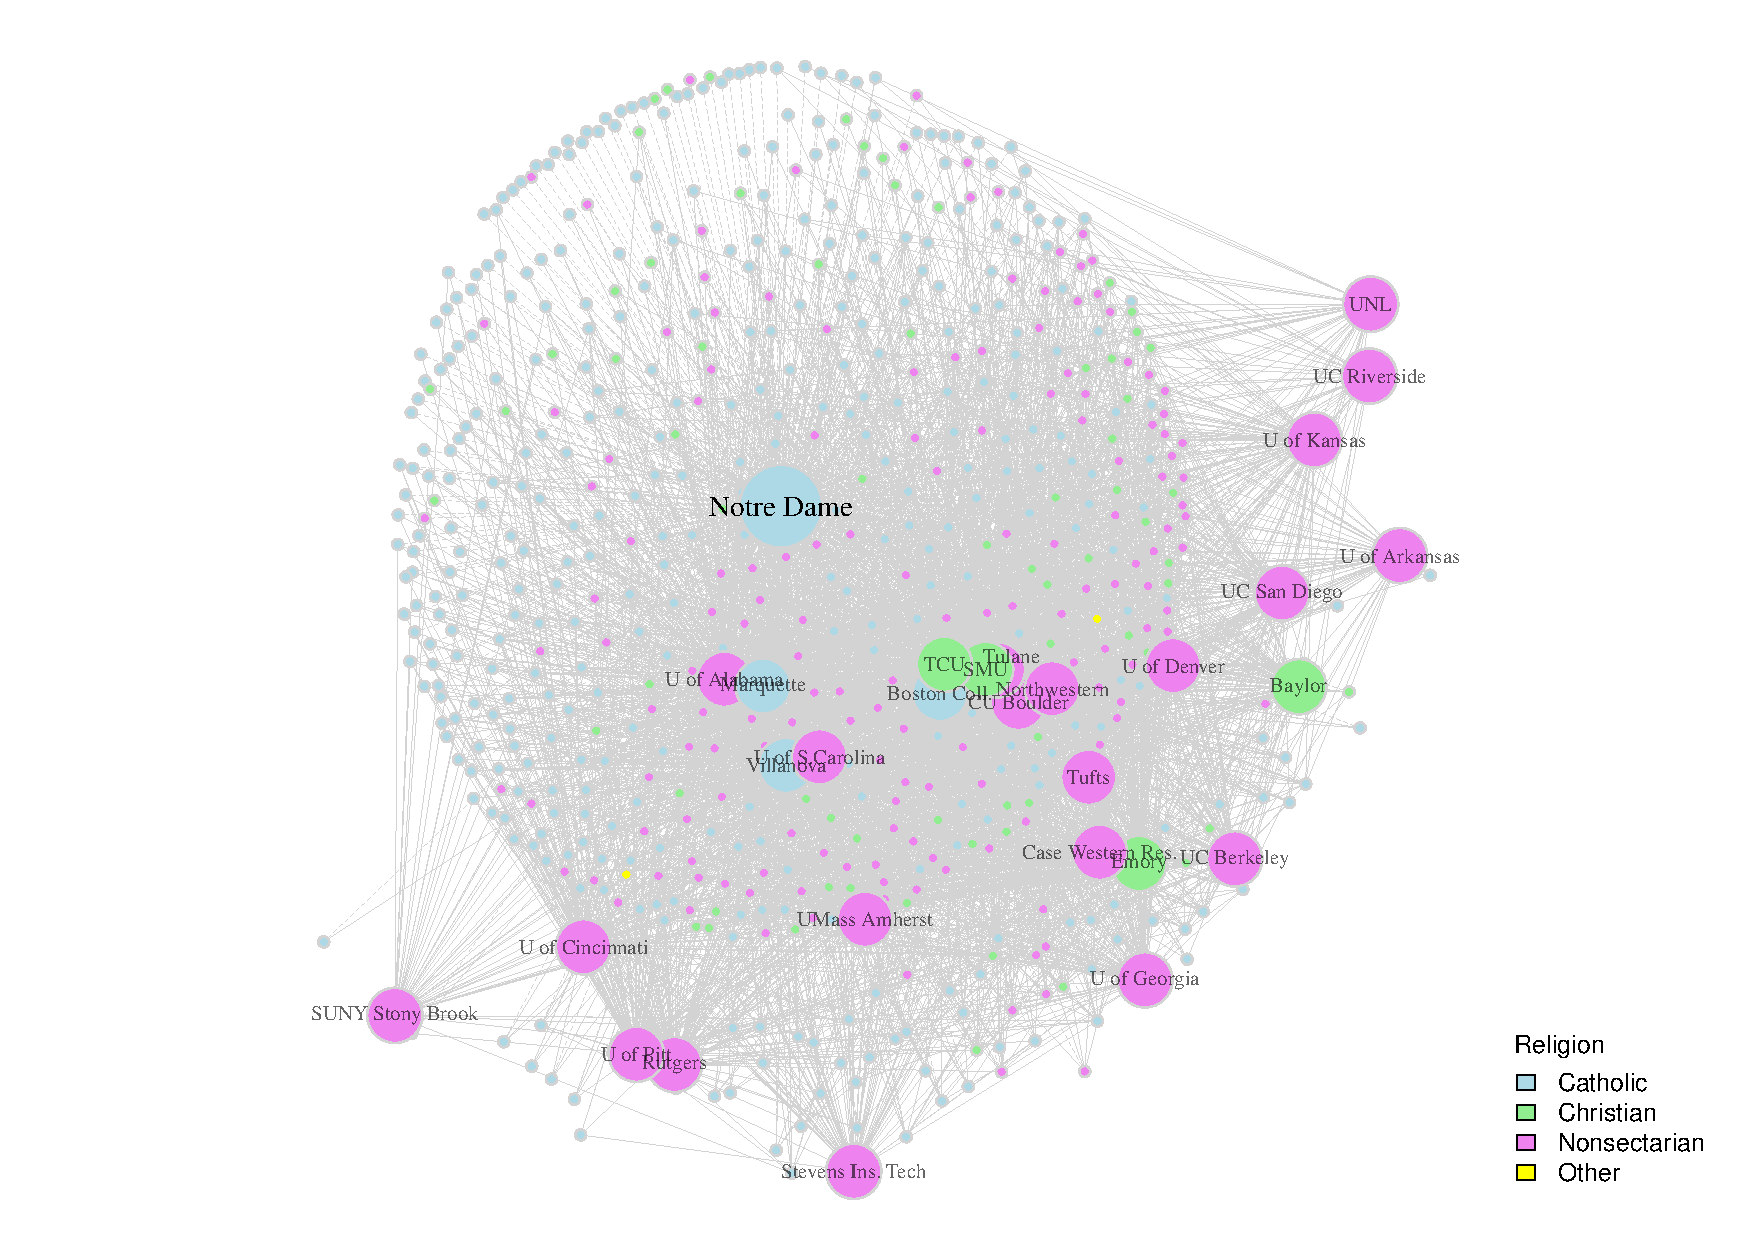
\includegraphics[width=2\linewidth]{../assets/figures/nd_religion} 

}

\caption{Order 2 ego network of University of Notre Dame, vertices colored by religion}\label{fig:nd-religion}
\end{figure}

\newpage

\begin{figure}

{\centering 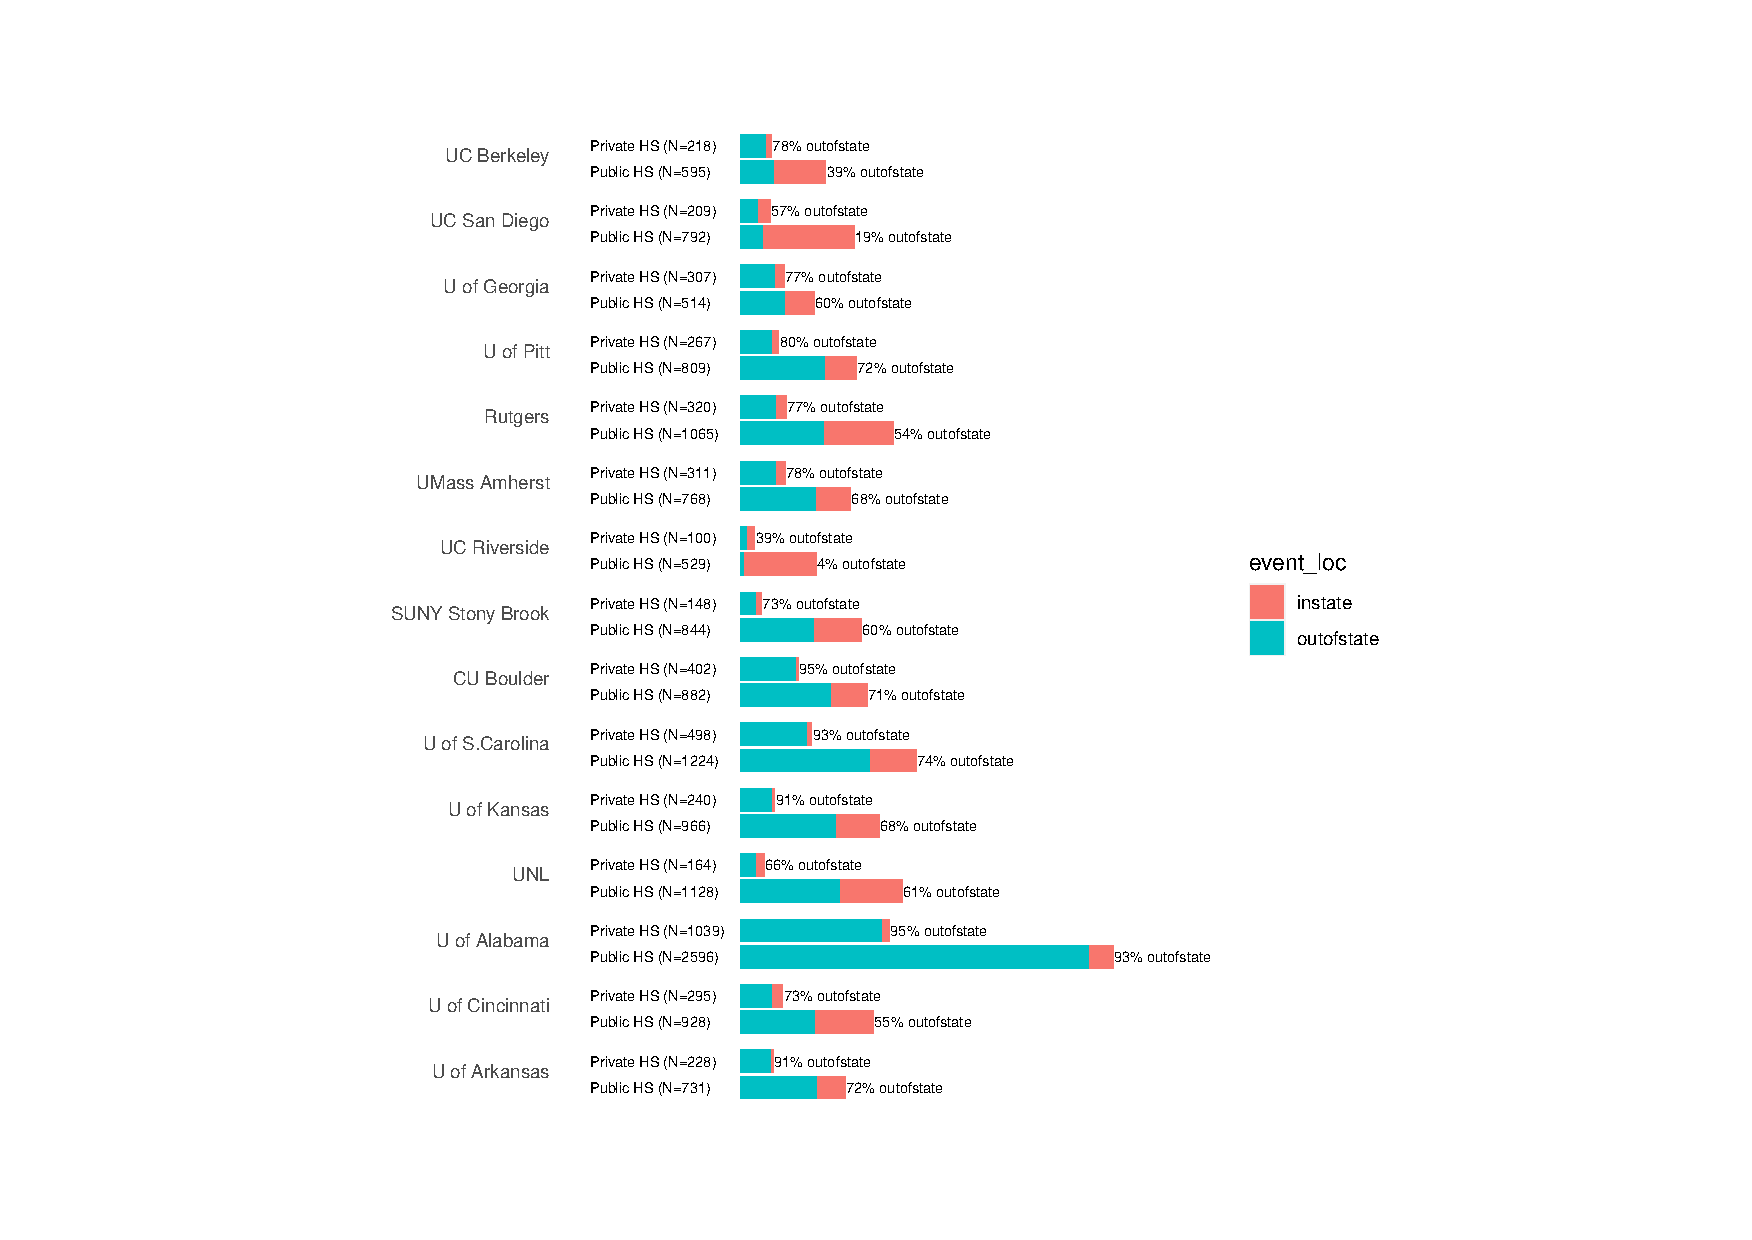
\includegraphics[width=2\linewidth]{../assets/figures/events_hs_count_pubu} 

}

\caption{Number of visits to public and private high schools by public research universities}\label{fig:events-hs-count-pubu}
\end{figure}

\newpage

\begin{figure}

{\centering 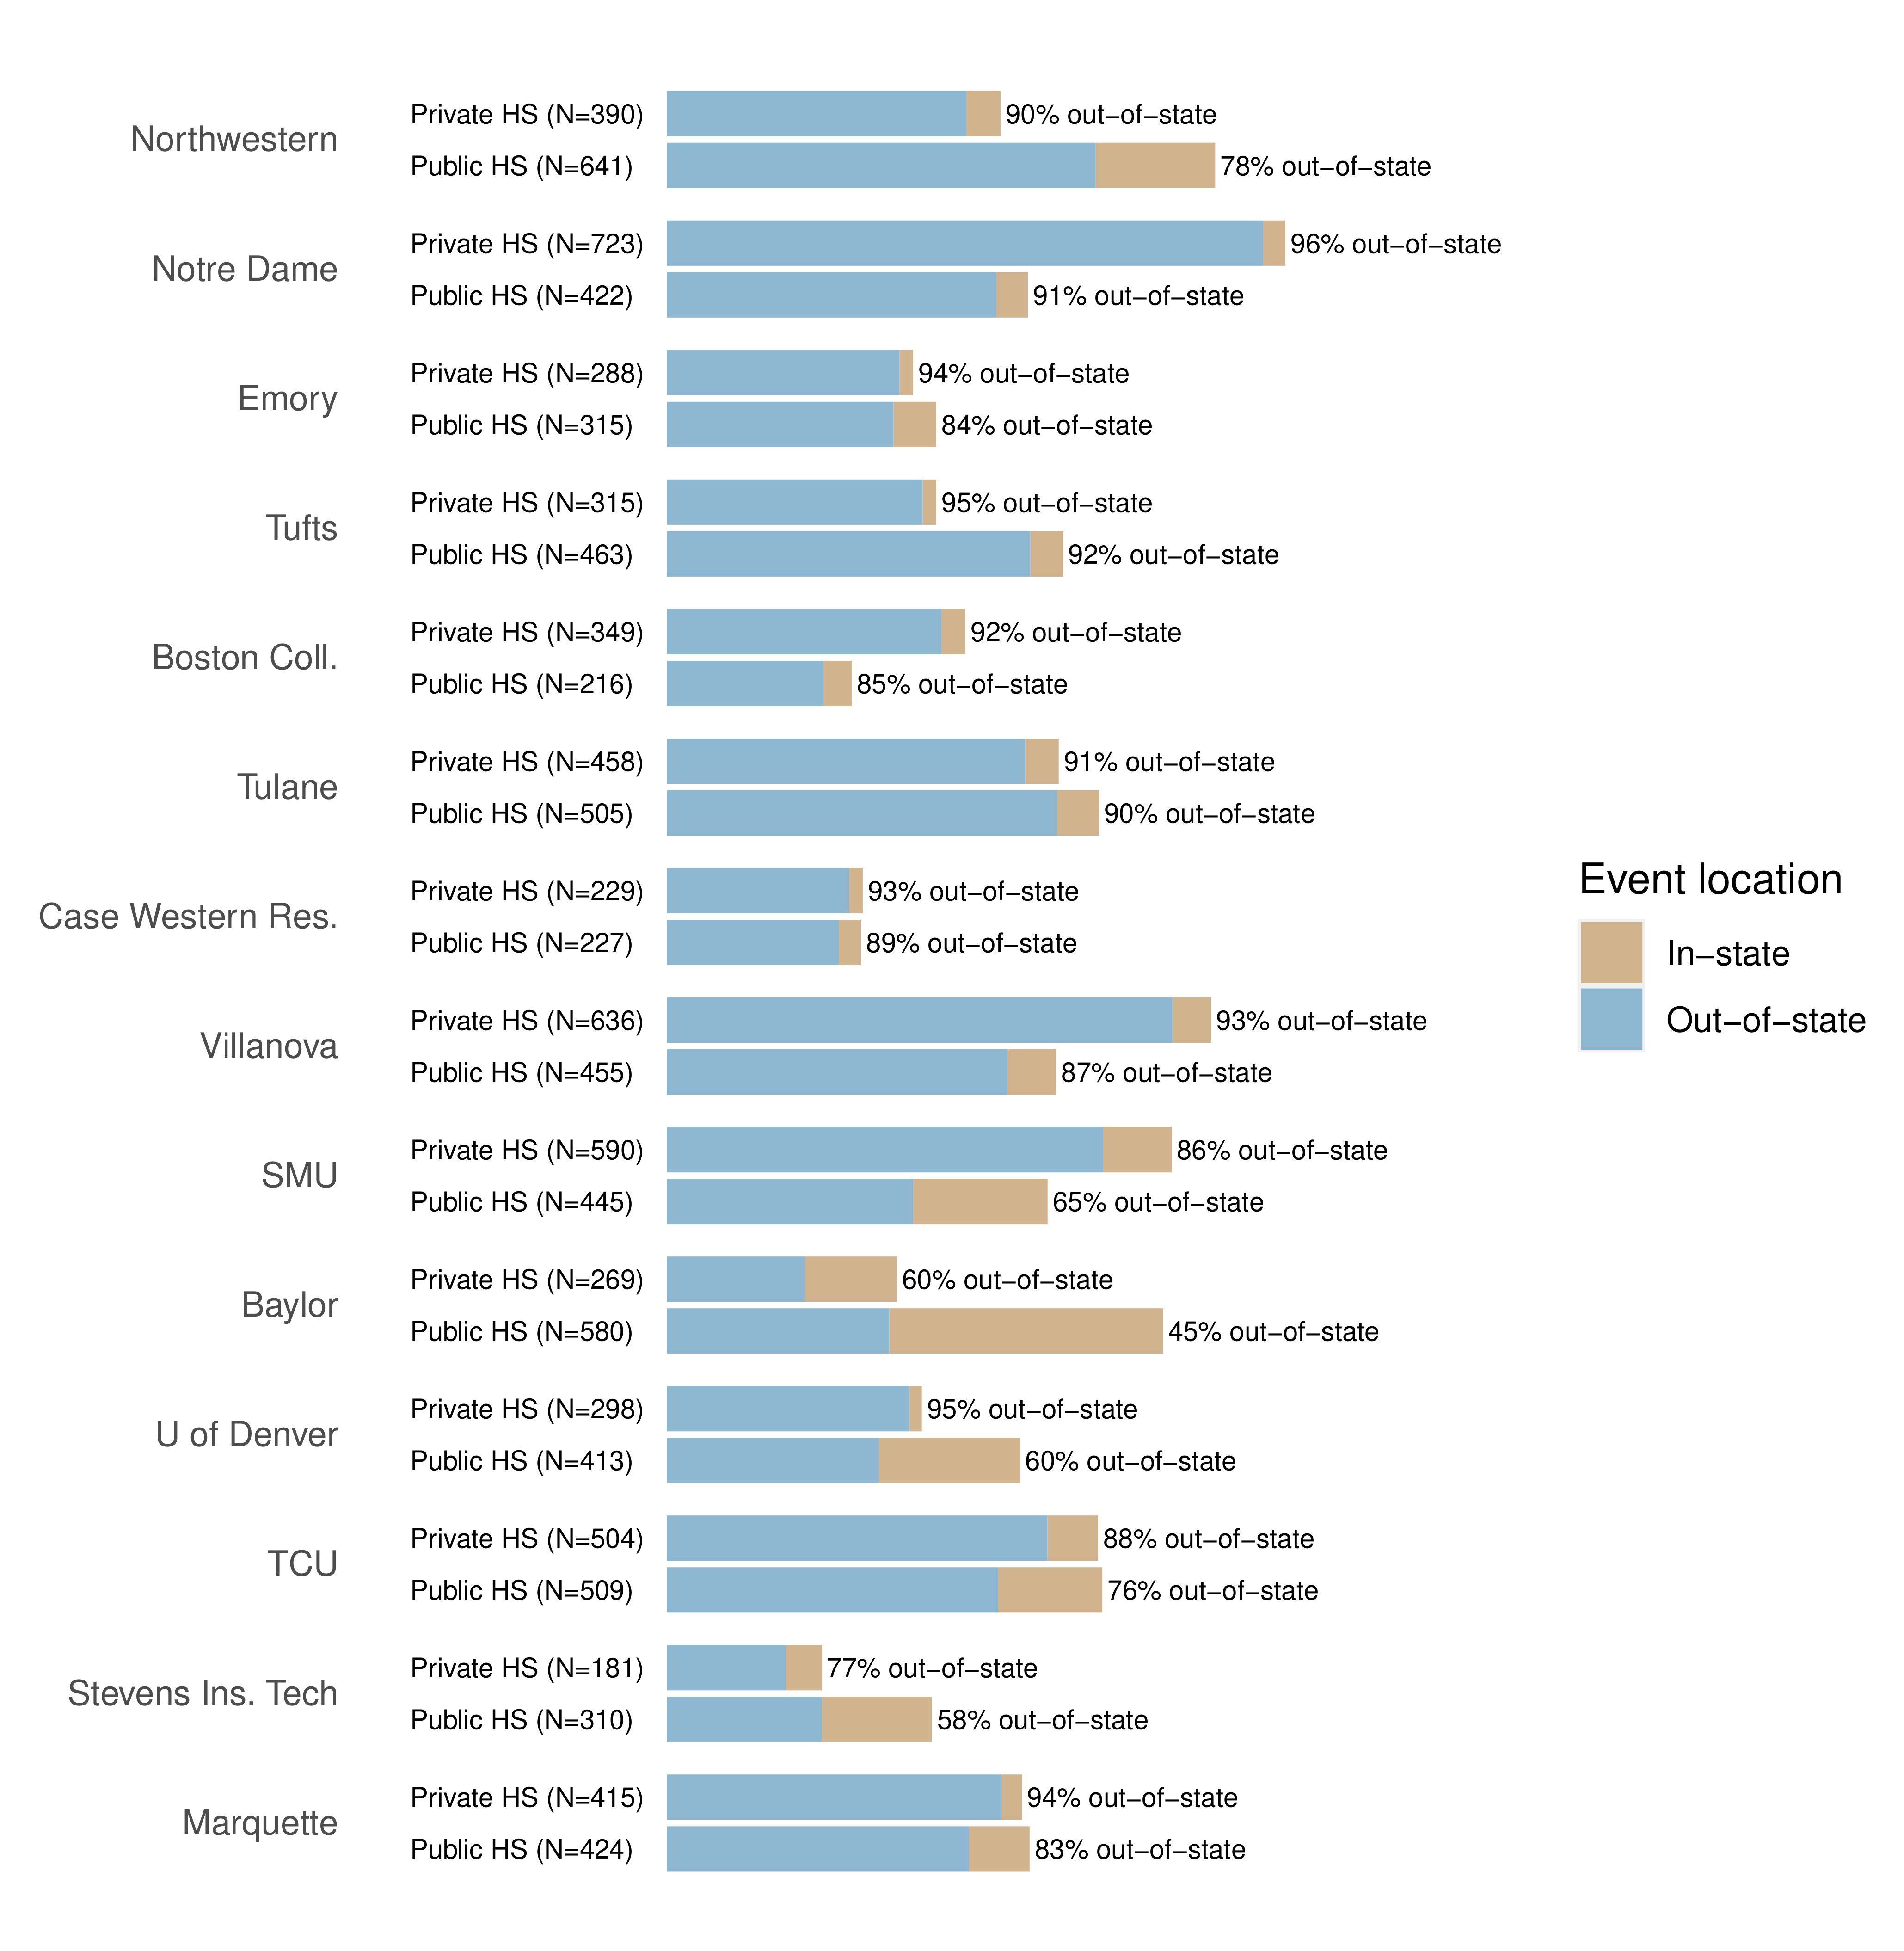
\includegraphics[width=2\linewidth]{../assets/figures/events_hs_count_privu} 

}

\caption{Number of visits to public and private high schools by selective private universities}\label{fig:events-hs-count-privu}
\end{figure}

\newpage

\begin{figure}

{\centering 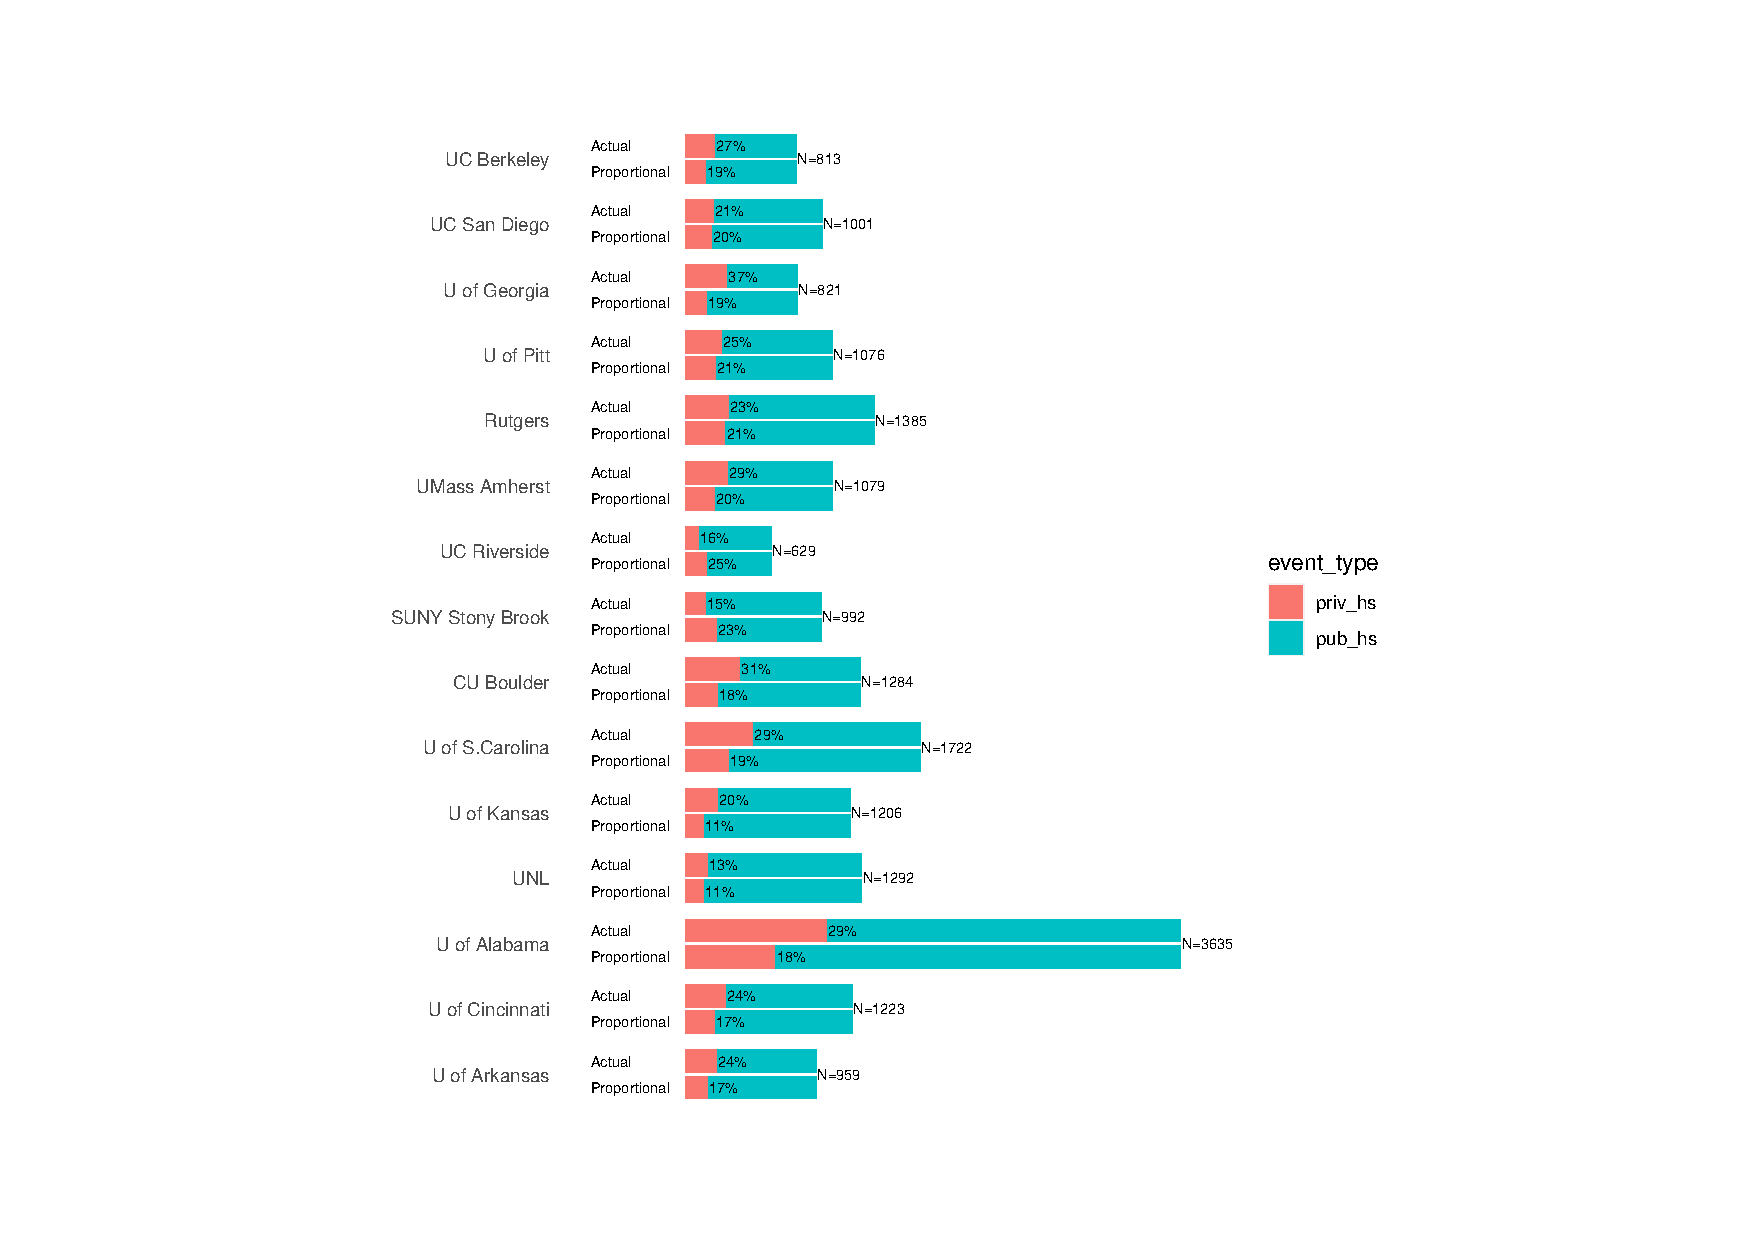
\includegraphics[width=2\linewidth]{../assets/figures/events_hs_actual_proportional_pubu} 

}

\caption{Actual versus proportional number of private school visits, public research universities}\label{fig:actual-proportional-pubu}
\end{figure}

\clearpage

\begin{figure}

{\centering 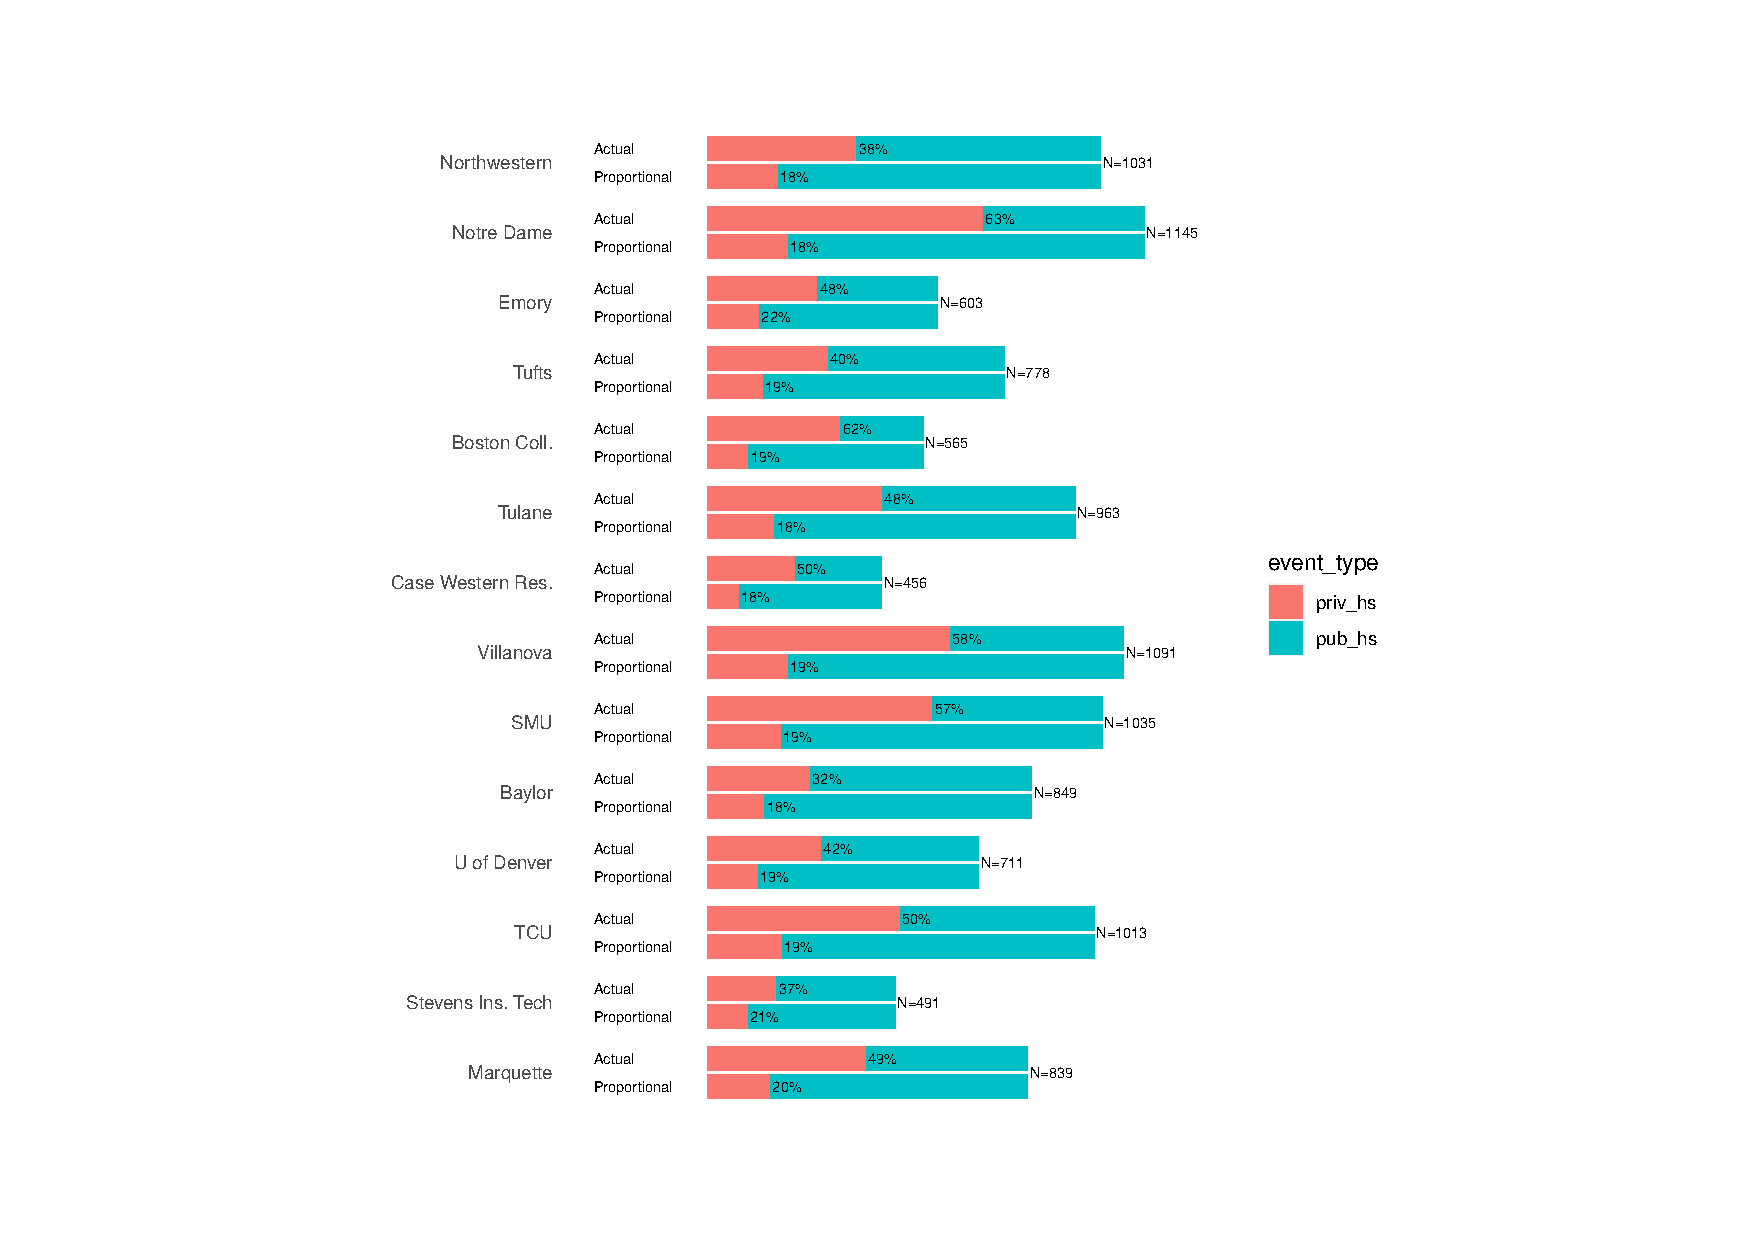
\includegraphics[width=2\linewidth]{../assets/figures/events_hs_actual_proportional_privu} 

}

\caption{Actual versus proportional number of private school visits, selective private universities}\label{fig:actual-proportional-privu}
\end{figure}

\newpage

\begin{figure}

{\centering 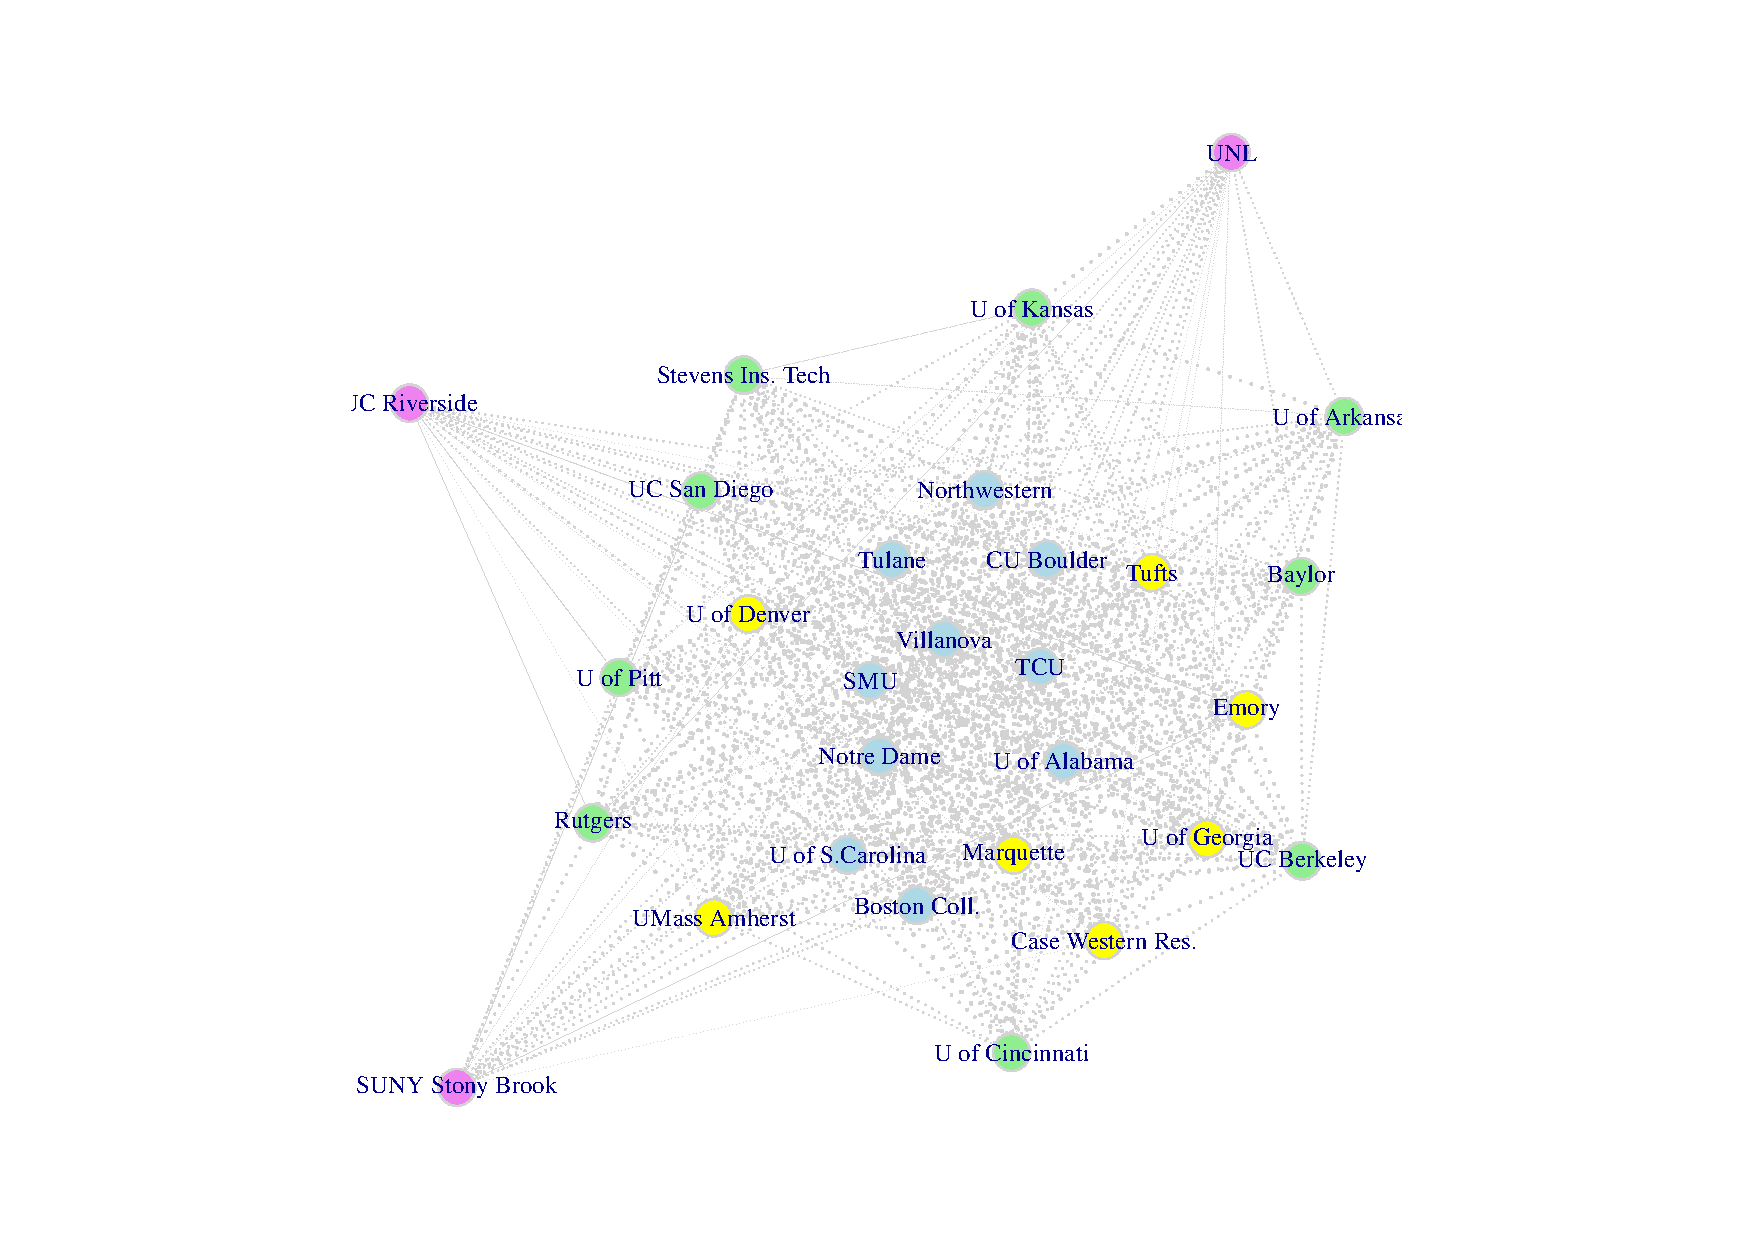
\includegraphics[width=2\linewidth]{../assets/figures/plot_1mode_u} 

}

\caption{One-mode network for public and private universities, colored by cluster}\label{fig:plot-1mode-u}
\end{figure}

\clearpage

\begin{figure}

{\centering 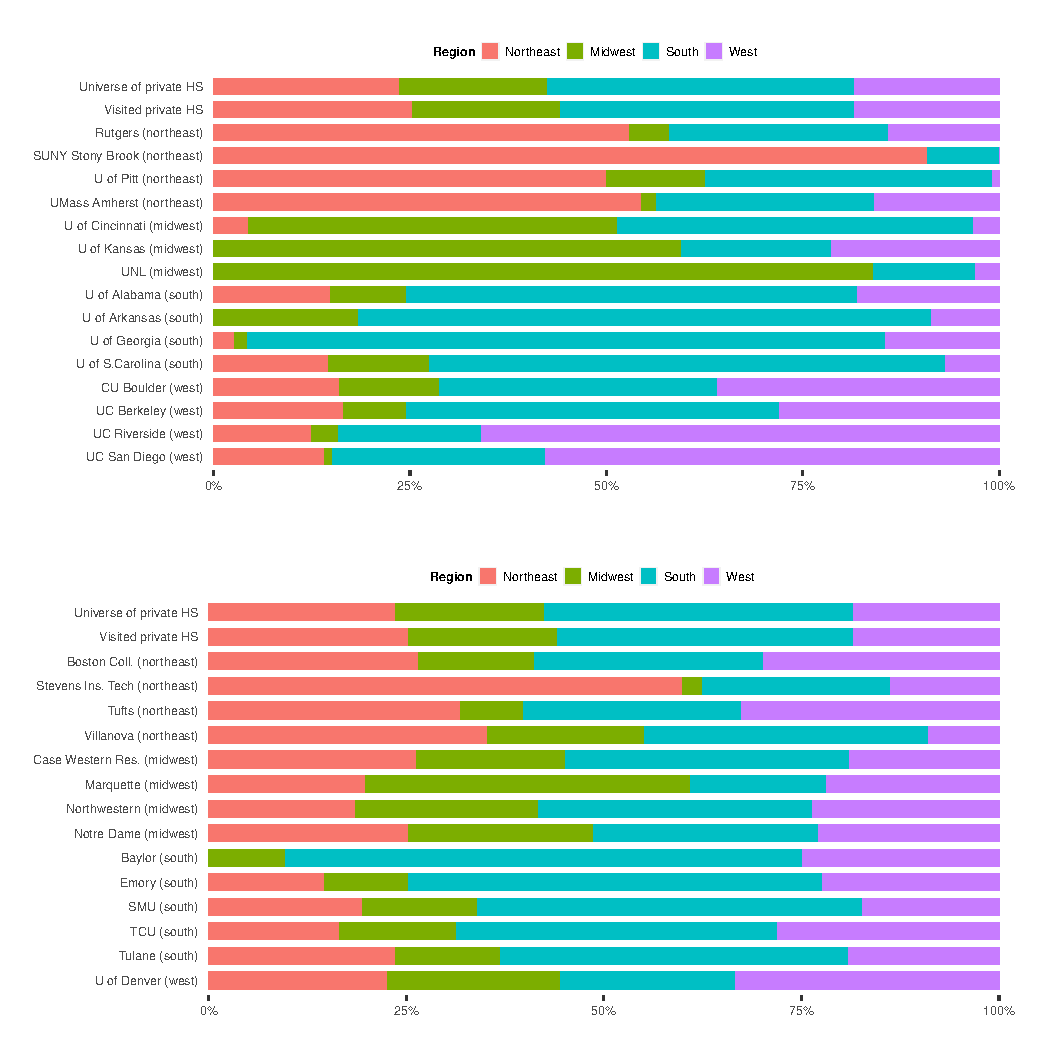
\includegraphics[width=2\linewidth]{../assets/figures/ego_network_region_pubu_privu} 

}

\caption{Geographic region of visited private high schools}\label{fig:region-pubu-privu}
\end{figure}

\newpage

\begin{figure}

{\centering 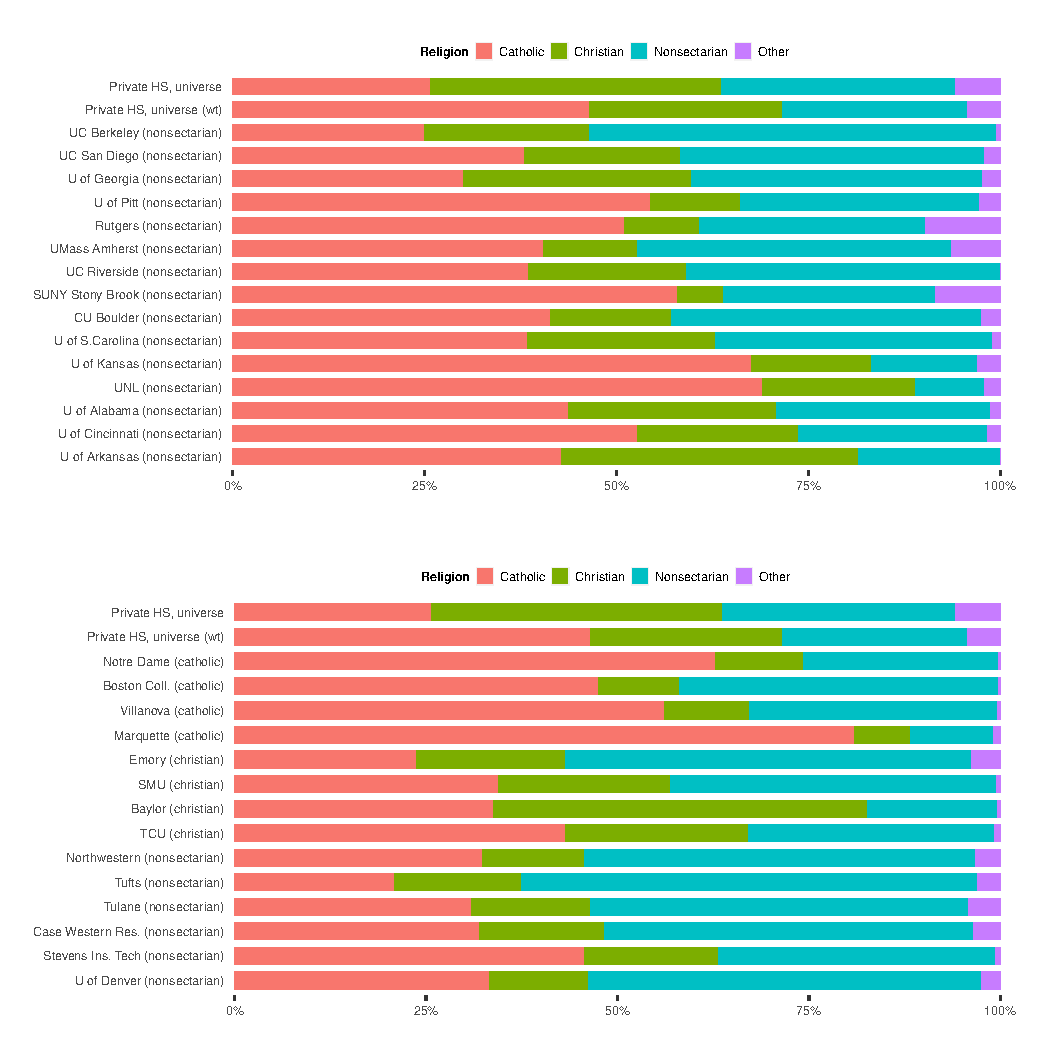
\includegraphics[width=2\linewidth]{../assets/figures/ego_network_religion_pubu_privu} 

}

\caption{Religious affiliation of visited private high schools}\label{fig:religion-pubu-privu}
\end{figure}

\newpage

\begin{figure}

{\centering 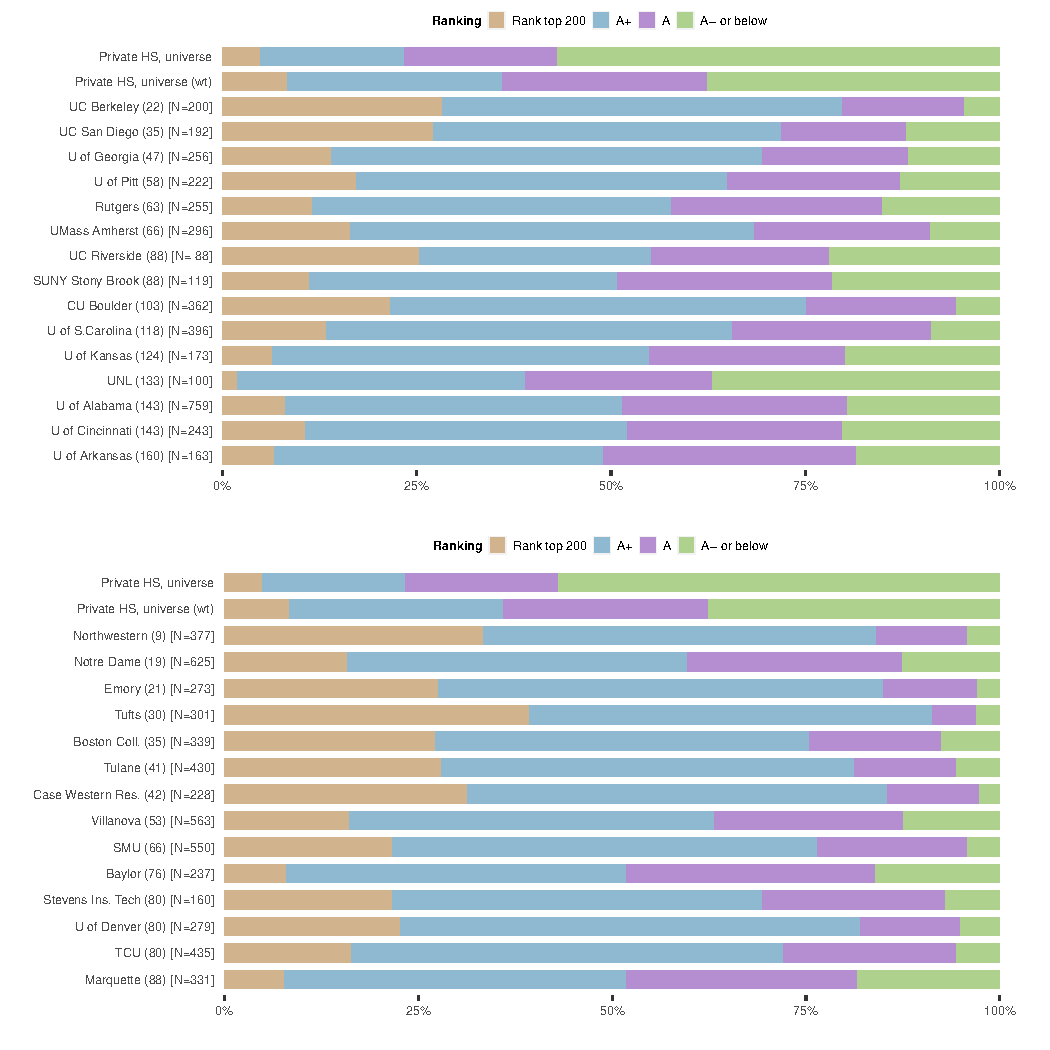
\includegraphics[width=2\linewidth]{../assets/figures/ego_network_rank_pubu_privu} 

}

\caption{High school ranking of visited private high schools}\label{fig:rank-pubu-privu}
\end{figure}

\newpage

\begin{figure}

{\centering 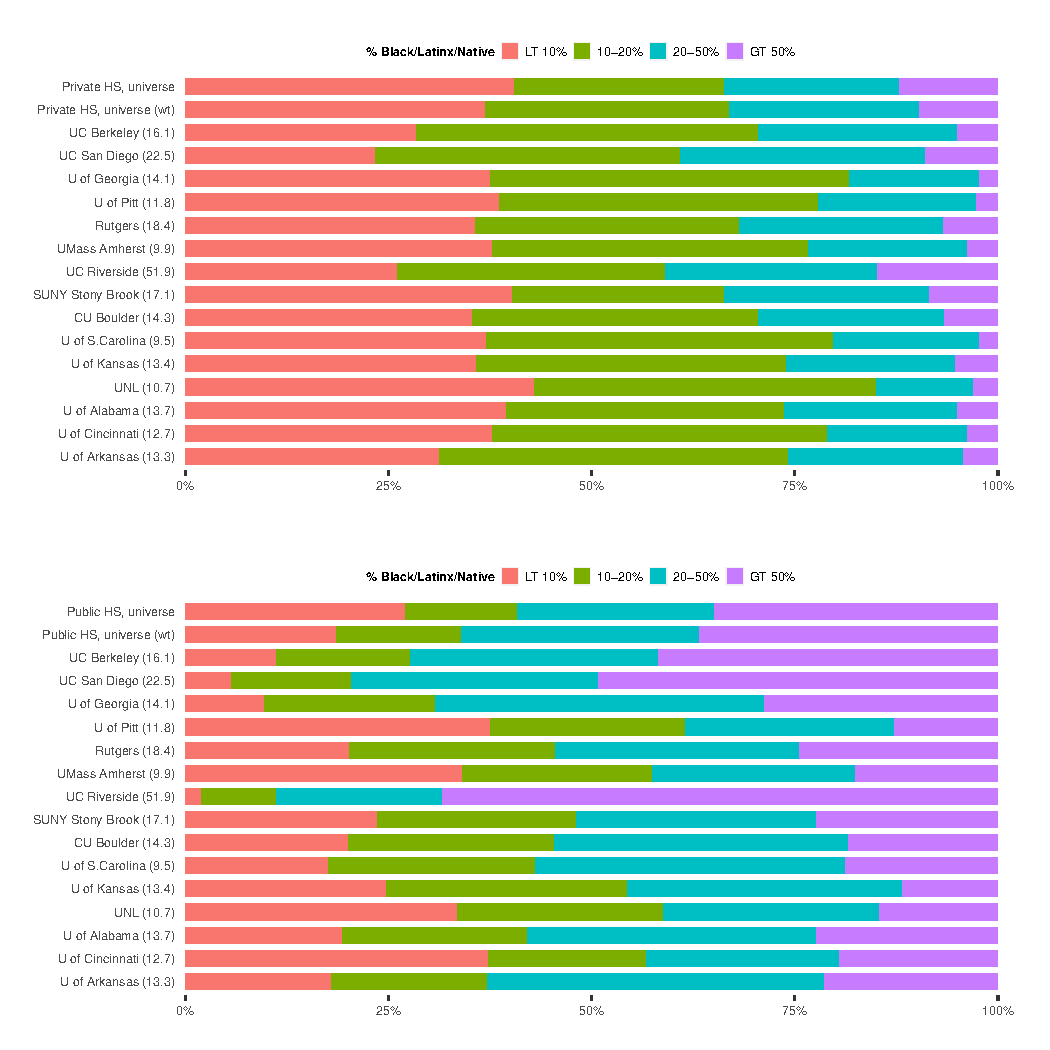
\includegraphics[width=2\linewidth]{../assets/figures/ego_network_race_pubu_privhs_pubhs} 

}

\caption{Percentage of students who identify as Black, Latinx, or Native at visited public high schools vs. visited private high schools, public research universities}\label{fig:race-pubu-privhs-pubhs}
\end{figure}

\newpage

\begin{figure}

{\centering 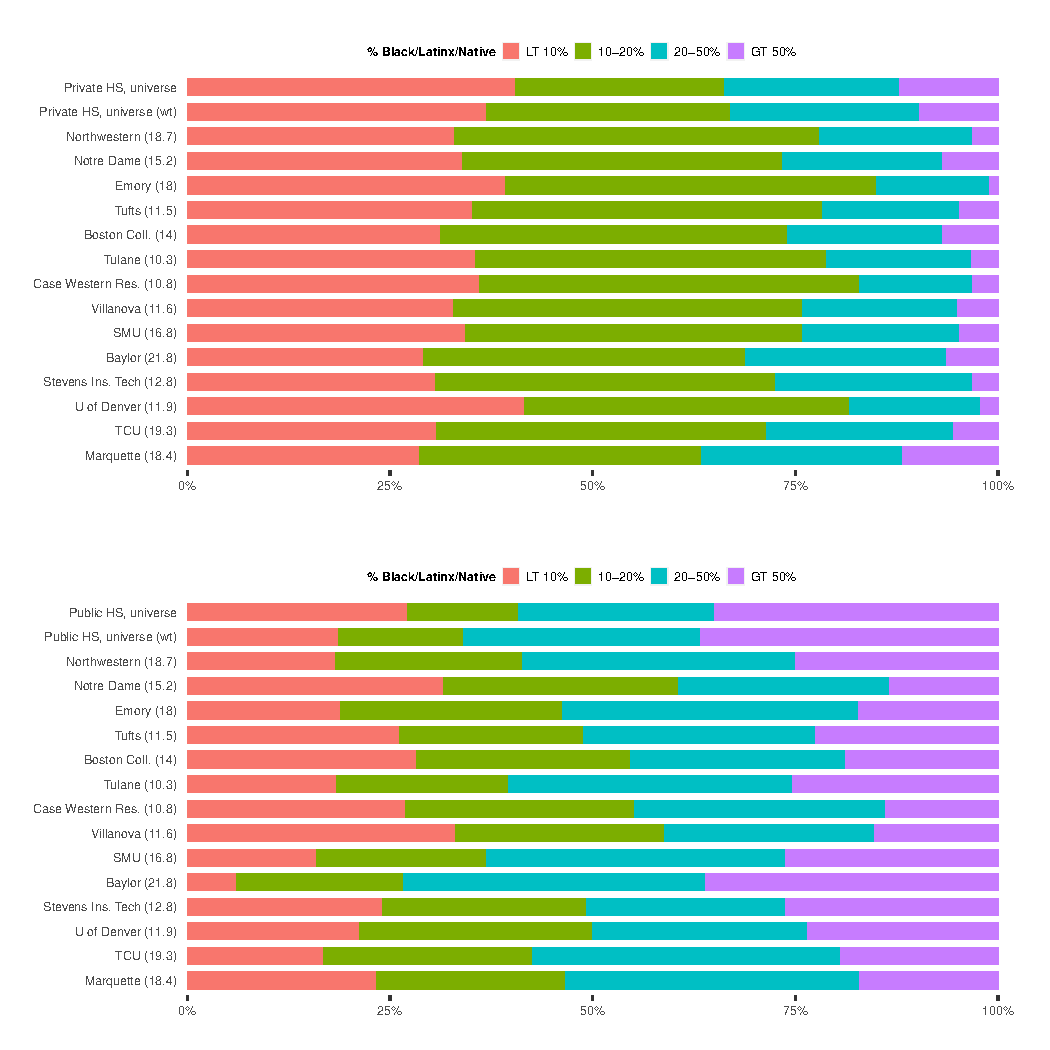
\includegraphics[width=2\linewidth]{../assets/figures/ego_network_race_privu_privhs_pubhs} 

}

\caption{Percentage of students who identify as Black, Latinx, or Native at visited public high schools vs. visited private high schools, selective private universities}\label{fig:race-privu-privhs-pubhs}
\end{figure}

\newpage

\begin{figure}

{\centering 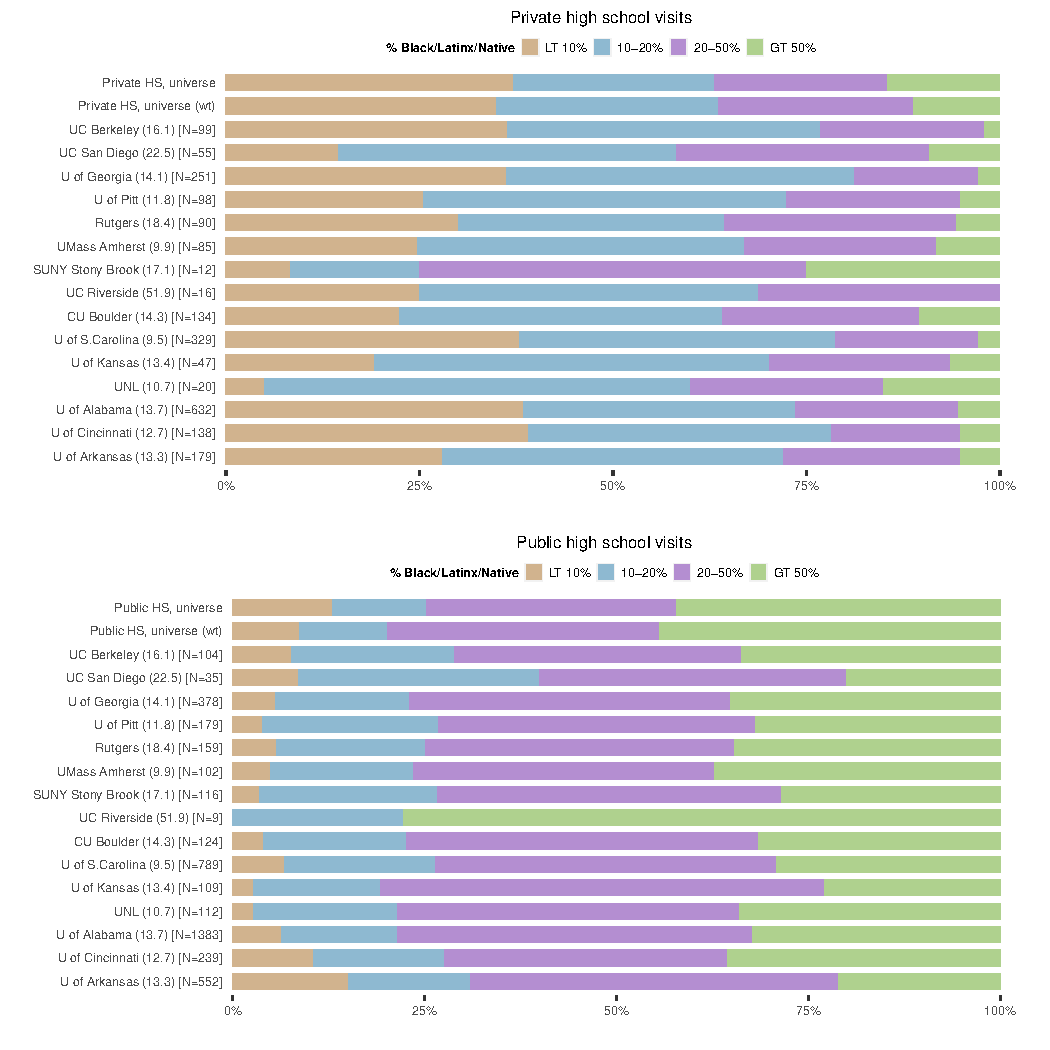
\includegraphics[width=2\linewidth]{../assets/figures/south_race_pubu_privhs_pubhs} 

}

\caption{Percentage of students who identify as Black, Latinx, or Native at visited public high schools in the South vs. visited private high schools in the South, public research universities}\label{fig:south-race-pubu-privhs-pubhs}
\end{figure}

\newpage

\begin{figure}

{\centering 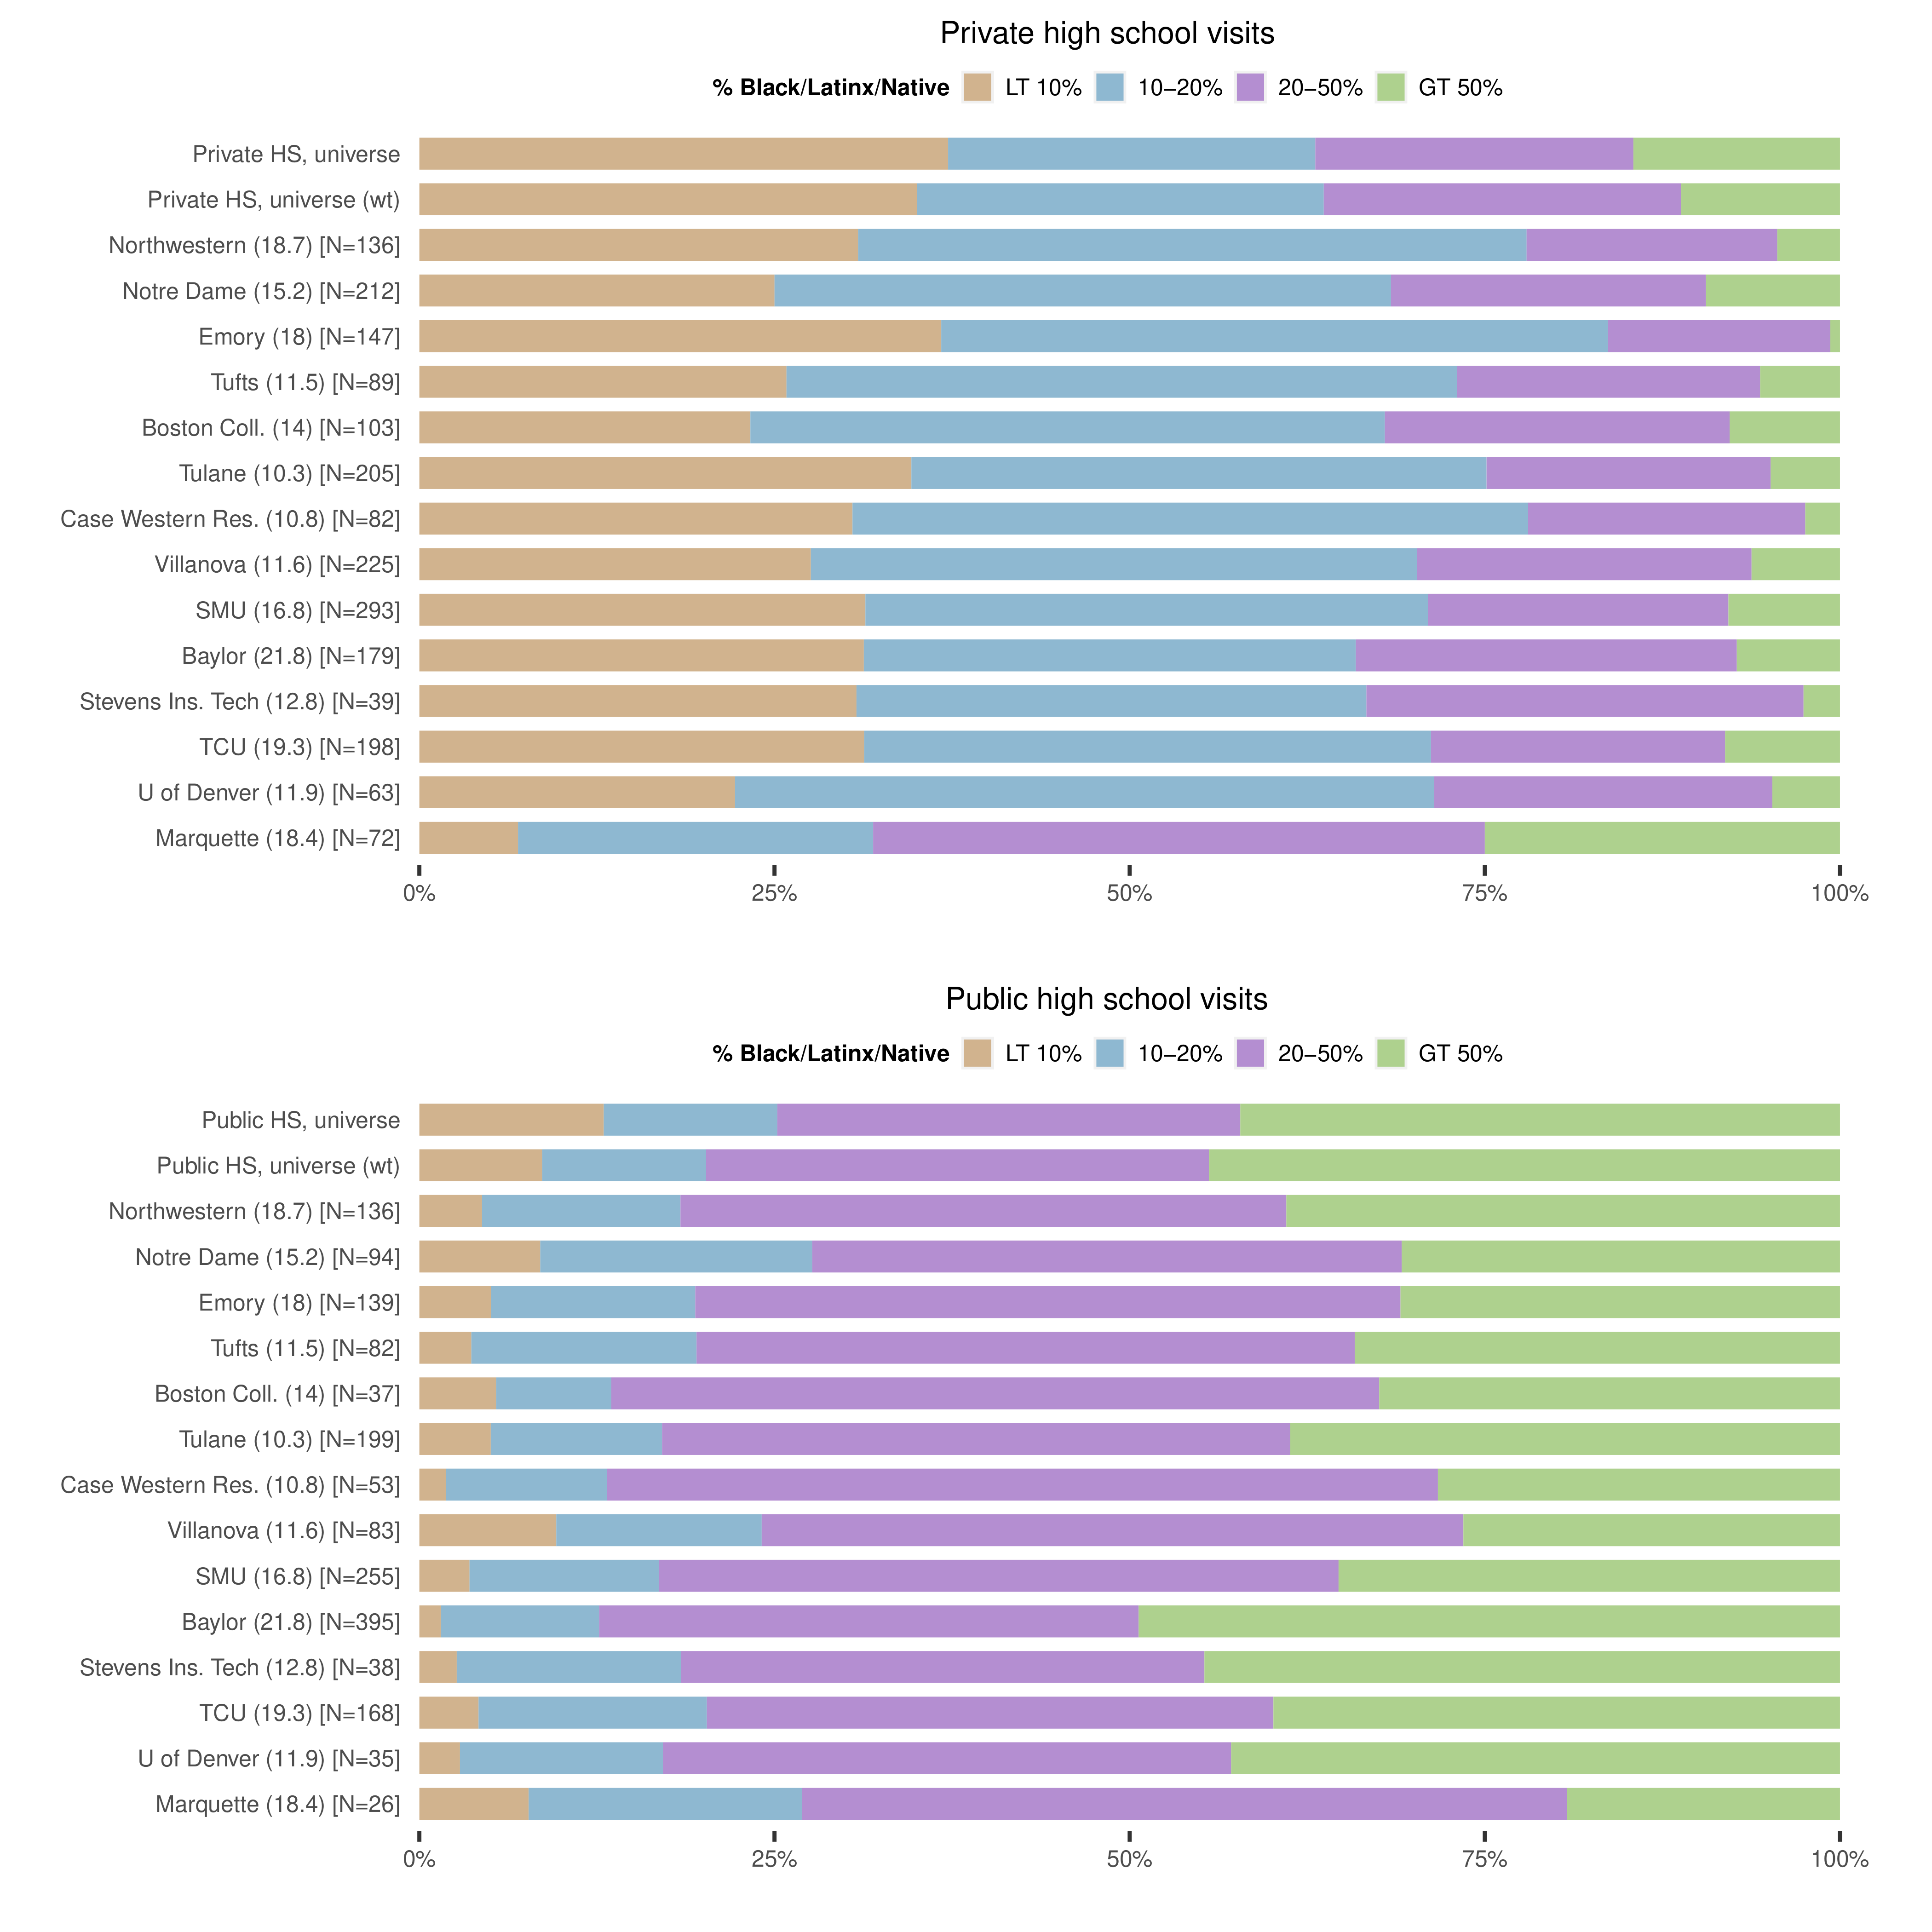
\includegraphics[width=2\linewidth]{../assets/figures/south_race_privu_privhs_pubhs} 

}

\caption{Percentage of students who identify as Black, Latinx, or Native at visited public high schools in the South vs. visited private high schools in the South, selective private universities}\label{fig:south-race-privu-privhs-pubhs}
\end{figure}



\beginsupplement
\clearpage
\newpage

\begin{table}

\caption{\label{tab:pubu-count-matrix}One-mode public university count matrix}
\centering
\resizebox{\linewidth}{!}{
\fontsize{13}{15}\selectfont
\begin{tabular}[t]{l>{\raggedleft\arraybackslash}p{6.5em}>{\raggedleft\arraybackslash}p{7em}>{\raggedleft\arraybackslash}p{5.5em}>{\raggedleft\arraybackslash}p{7.5em}>{\raggedleft\arraybackslash}p{6em}>{\raggedleft\arraybackslash}p{5em}>{\raggedleft\arraybackslash}p{7em}>{\raggedleft\arraybackslash}p{5em}>{\raggedleft\arraybackslash}p{6em}>{\raggedleft\arraybackslash}p{6.5em}>{\raggedleft\arraybackslash}p{5.5em}>{\raggedleft\arraybackslash}p{6.5em}>{\raggedleft\arraybackslash}p{8.8em}>{\raggedleft\arraybackslash}p{5em}>{\raggedleft\arraybackslash}p{6em}}
\toprule
\multicolumn{1}{c}{ } & \multicolumn{1}{>{\centering\arraybackslash}p{6.5em}}{U of Alabama (N=759)} & \multicolumn{1}{>{\centering\arraybackslash}p{7em}}{U of S.Carolina (N=396)} & \multicolumn{1}{>{\centering\arraybackslash}p{5.5em}}{CU Boulder (N=362)} & \multicolumn{1}{>{\centering\arraybackslash}p{7.5em}}{UMass Amherst (N=296)} & \multicolumn{1}{>{\centering\arraybackslash}p{6em}}{U of Georgia (N=256)} & \multicolumn{1}{>{\centering\arraybackslash}p{5em}}{Rutgers (N=255)} & \multicolumn{1}{>{\centering\arraybackslash}p{7em}}{U of Cincinnati (N=243)} & \multicolumn{1}{>{\centering\arraybackslash}p{5em}}{U of Pitt (N=222)} & \multicolumn{1}{>{\centering\arraybackslash}p{6em}}{UC Berkeley (N=200)} & \multicolumn{1}{>{\centering\arraybackslash}p{6.5em}}{UC San Diego (N=192)} & \multicolumn{1}{>{\centering\arraybackslash}p{5.5em}}{U of Kansas (N=173)} & \multicolumn{1}{>{\centering\arraybackslash}p{6.5em}}{U of Arkansas (N=163)} & \multicolumn{1}{>{\centering\arraybackslash}p{8.8em}}{SUNY Stony Brook (N=119)} & \multicolumn{1}{>{\centering\arraybackslash}p{5em}}{UNL (N=100)} & \multicolumn{1}{>{\centering\arraybackslash}p{6em}}{UC Riverside (N=88)}\\
\midrule
U of Alabama (N=759) & 759 & 284 & 210 & 149 & 169 & 120 & 124 & 125 & 112 & 100 & 93 & 100 & 43 & 31 & 34\\
U of S.Carolina (N=396) & 284 & 396 & 155 & 108 & 140 & 74 & 110 & 99 & 84 & 59 & 58 & 57 & 27 & 20 & 19\\
CU Boulder (N=362) & 210 & 155 & 362 & 115 & 88 & 76 & 69 & 92 & 77 & 98 & 74 & 51 & 21 & 25 & 28\\
UMass Amherst (N=296) & 149 & 108 & 115 & 296 & 57 & 93 & 27 & 56 & 45 & 57 & 18 & 14 & 57 & 4 & 18\\
U of Georgia (N=256) & 169 & 140 & 88 & 57 & 256 & 24 & 73 & 48 & 64 & 38 & 39 & 59 & 7 & 13 & 16\\
Rutgers (N=255) & 120 & 74 & 76 & 93 & 24 & 255 & 35 & 74 & 41 & 43 & 20 & 5 & 48 & 10 & 10\\
U of Cincinnati (N=243) & 124 & 110 & 69 & 27 & 73 & 35 & 243 & 56 & 33 & 24 & 29 & 37 & 5 & 18 & 8\\
U of Pitt (N=222) & 125 & 99 & 92 & 56 & 48 & 74 & 56 & 222 & 41 & 28 & 32 & 26 & 27 & 15 & 11\\
UC Berkeley (N=200) & 112 & 84 & 77 & 45 & 64 & 41 & 33 & 41 & 200 & 61 & 30 & 26 & 9 & 8 & 20\\
UC San Diego (N=192) & 100 & 59 & 98 & 57 & 38 & 43 & 24 & 28 & 61 & 192 & 29 & 22 & 11 & 3 & 35\\
U of Kansas (N=173) & 93 & 58 & 74 & 18 & 39 & 20 & 29 & 32 & 30 & 29 & 173 & 62 & 0 & 61 & 8\\
U of Arkansas (N=163) & 100 & 57 & 51 & 14 & 59 & 5 & 37 & 26 & 26 & 22 & 62 & 163 & 1 & 24 & 9\\
SUNY Stony Brook (N=119) & 43 & 27 & 21 & 57 & 7 & 48 & 5 & 27 & 9 & 11 & 0 & 1 & 119 & 0 & 4\\
UNL (N=100) & 31 & 20 & 25 & 4 & 13 & 10 & 18 & 15 & 8 & 3 & 61 & 24 & 0 & 100 & 0\\
UC Riverside (N=88) & 34 & 19 & 28 & 18 & 16 & 10 & 8 & 11 & 20 & 35 & 8 & 9 & 4 & 0 & 88\\
\bottomrule
\end{tabular}}
\end{table}

\begin{table}

\caption{\label{tab:privu-count-matrix}One-mode private universities count matrix}
\centering
\resizebox{\linewidth}{!}{
\fontsize{13}{15}\selectfont
\begin{tabular}[t]{l>{\raggedleft\arraybackslash}p{7em}>{\raggedleft\arraybackslash}p{7em}>{\raggedleft\arraybackslash}p{6em}>{\raggedleft\arraybackslash}p{6em}>{\raggedleft\arraybackslash}p{6em}>{\raggedleft\arraybackslash}p{7em}>{\raggedleft\arraybackslash}p{7em}>{\raggedleft\arraybackslash}p{7em}>{\raggedleft\arraybackslash}p{6em}>{\raggedleft\arraybackslash}p{7em}>{\raggedleft\arraybackslash}p{6em}>{\raggedleft\arraybackslash}p{6em}>{\raggedleft\arraybackslash}p{8.5em}>{\raggedleft\arraybackslash}p{8.5em}}
\toprule
\multicolumn{1}{c}{ } & \multicolumn{1}{>{\centering\arraybackslash}p{7em}}{Notre Dame (N=625)} & \multicolumn{1}{>{\centering\arraybackslash}p{7em}}{Villanova (N=563)} & \multicolumn{1}{>{\centering\arraybackslash}p{6em}}{SMU (N=550)} & \multicolumn{1}{>{\centering\arraybackslash}p{6em}}{TCU (N=435)} & \multicolumn{1}{>{\centering\arraybackslash}p{6em}}{Tulane (N=430)} & \multicolumn{1}{>{\centering\arraybackslash}p{7em}}{Northwestern (N=377)} & \multicolumn{1}{>{\centering\arraybackslash}p{7em}}{Boston Coll. (N=339)} & \multicolumn{1}{>{\centering\arraybackslash}p{7em}}{Marquette (N=331)} & \multicolumn{1}{>{\centering\arraybackslash}p{6em}}{Tufts (N=301)} & \multicolumn{1}{>{\centering\arraybackslash}p{7em}}{U of Denver (N=279)} & \multicolumn{1}{>{\centering\arraybackslash}p{6em}}{Emory (N=273)} & \multicolumn{1}{>{\centering\arraybackslash}p{6em}}{Baylor (N=237)} & \multicolumn{1}{>{\centering\arraybackslash}p{8.5em}}{Case Western Res. (N=228)} & \multicolumn{1}{>{\centering\arraybackslash}p{8.5em}}{Stevens Ins. Tech (N=160)}\\
\midrule
Notre Dame (N=625) & 625 & 338 & 293 & 253 & 223 & 224 & 235 & 231 & 177 & 164 & 145 & 99 & 133 & 79\\
Villanova (N=563) & 338 & 563 & 291 & 224 & 218 & 214 & 208 & 205 & 161 & 143 & 147 & 101 & 142 & 103\\
SMU (N=550) & 293 & 291 & 550 & 290 & 275 & 243 & 218 & 151 & 189 & 177 & 176 & 154 & 134 & 88\\
TCU (N=435) & 253 & 224 & 290 & 435 & 199 & 177 & 168 & 150 & 141 & 151 & 122 & 133 & 98 & 66\\
Tulane (N=430) & 223 & 218 & 275 & 199 & 430 & 219 & 173 & 103 & 190 & 142 & 143 & 79 & 131 & 56\\
Northwestern (N=377) & 224 & 214 & 243 & 177 & 219 & 377 & 172 & 114 & 169 & 139 & 128 & 75 & 122 & 55\\
Boston Coll. (N=339) & 235 & 208 & 218 & 168 & 173 & 172 & 339 & 133 & 158 & 135 & 113 & 64 & 100 & 60\\
Marquette (N=331) & 231 & 205 & 151 & 150 & 103 & 114 & 133 & 331 & 77 & 97 & 52 & 62 & 66 & 43\\
Tufts (N=301) & 177 & 161 & 189 & 141 & 190 & 169 & 158 & 77 & 301 & 114 & 117 & 52 & 108 & 66\\
U of Denver (N=279) & 164 & 143 & 177 & 151 & 142 & 139 & 135 & 97 & 114 & 279 & 82 & 57 & 72 & 44\\
Emory (N=273) & 145 & 147 & 176 & 122 & 143 & 128 & 113 & 52 & 117 & 82 & 273 & 39 & 98 & 42\\
Baylor (N=237) & 99 & 101 & 154 & 133 & 79 & 75 & 64 & 62 & 52 & 57 & 39 & 237 & 50 & 23\\
Case Western Res. (N=228) & 133 & 142 & 134 & 98 & 131 & 122 & 100 & 66 & 108 & 72 & 98 & 50 & 228 & 41\\
Stevens Ins. Tech (N=160) & 79 & 103 & 88 & 66 & 56 & 55 & 60 & 43 & 66 & 44 & 42 & 23 & 41 & 160\\
\bottomrule
\end{tabular}}
\end{table}

\newpage

\begin{figure}

{\centering 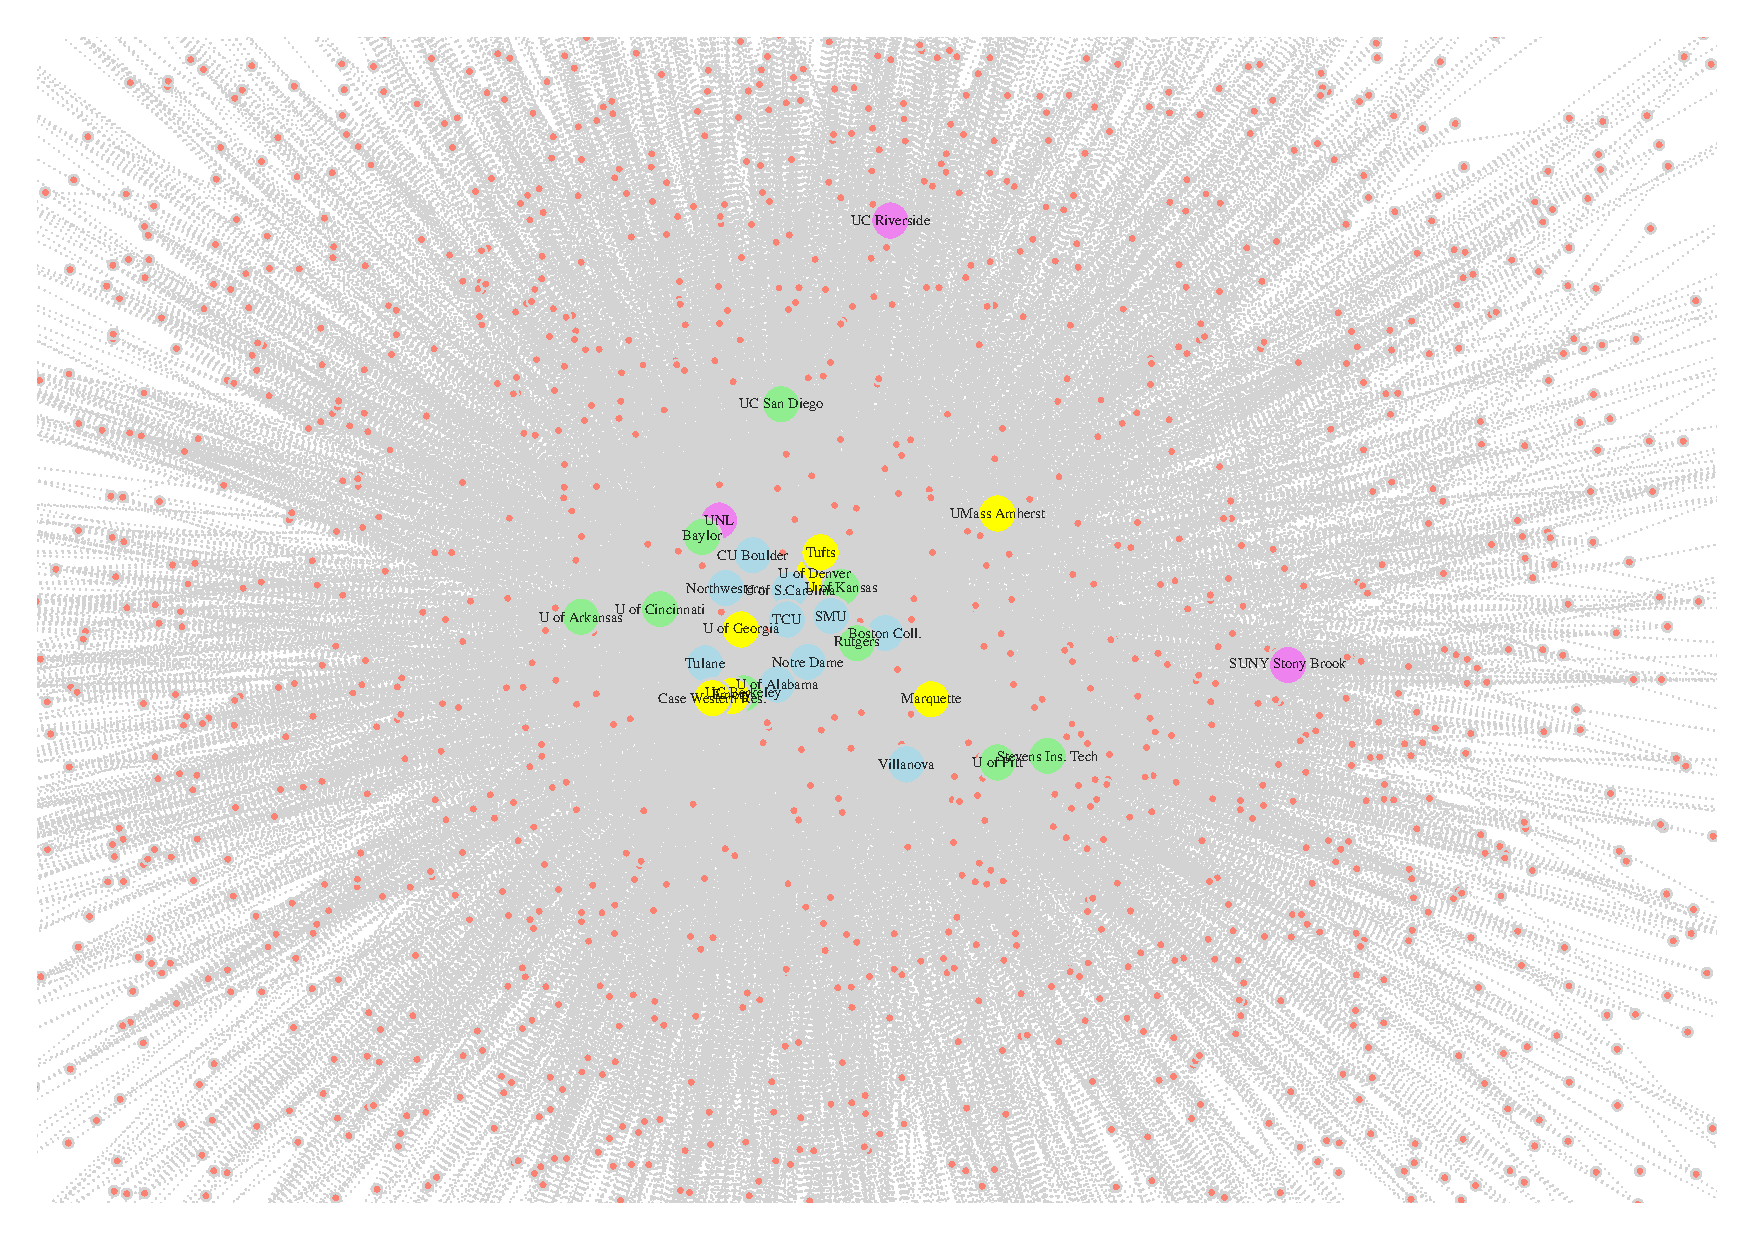
\includegraphics[width=2\linewidth]{../assets/figures/plot_2mode_u} 

}

\caption{Two-mode network for private high schools and all visiting universities, colored by cluster}\label{fig:plot-2mode}
\end{figure}


\newpage

\begin{figure}

{\centering 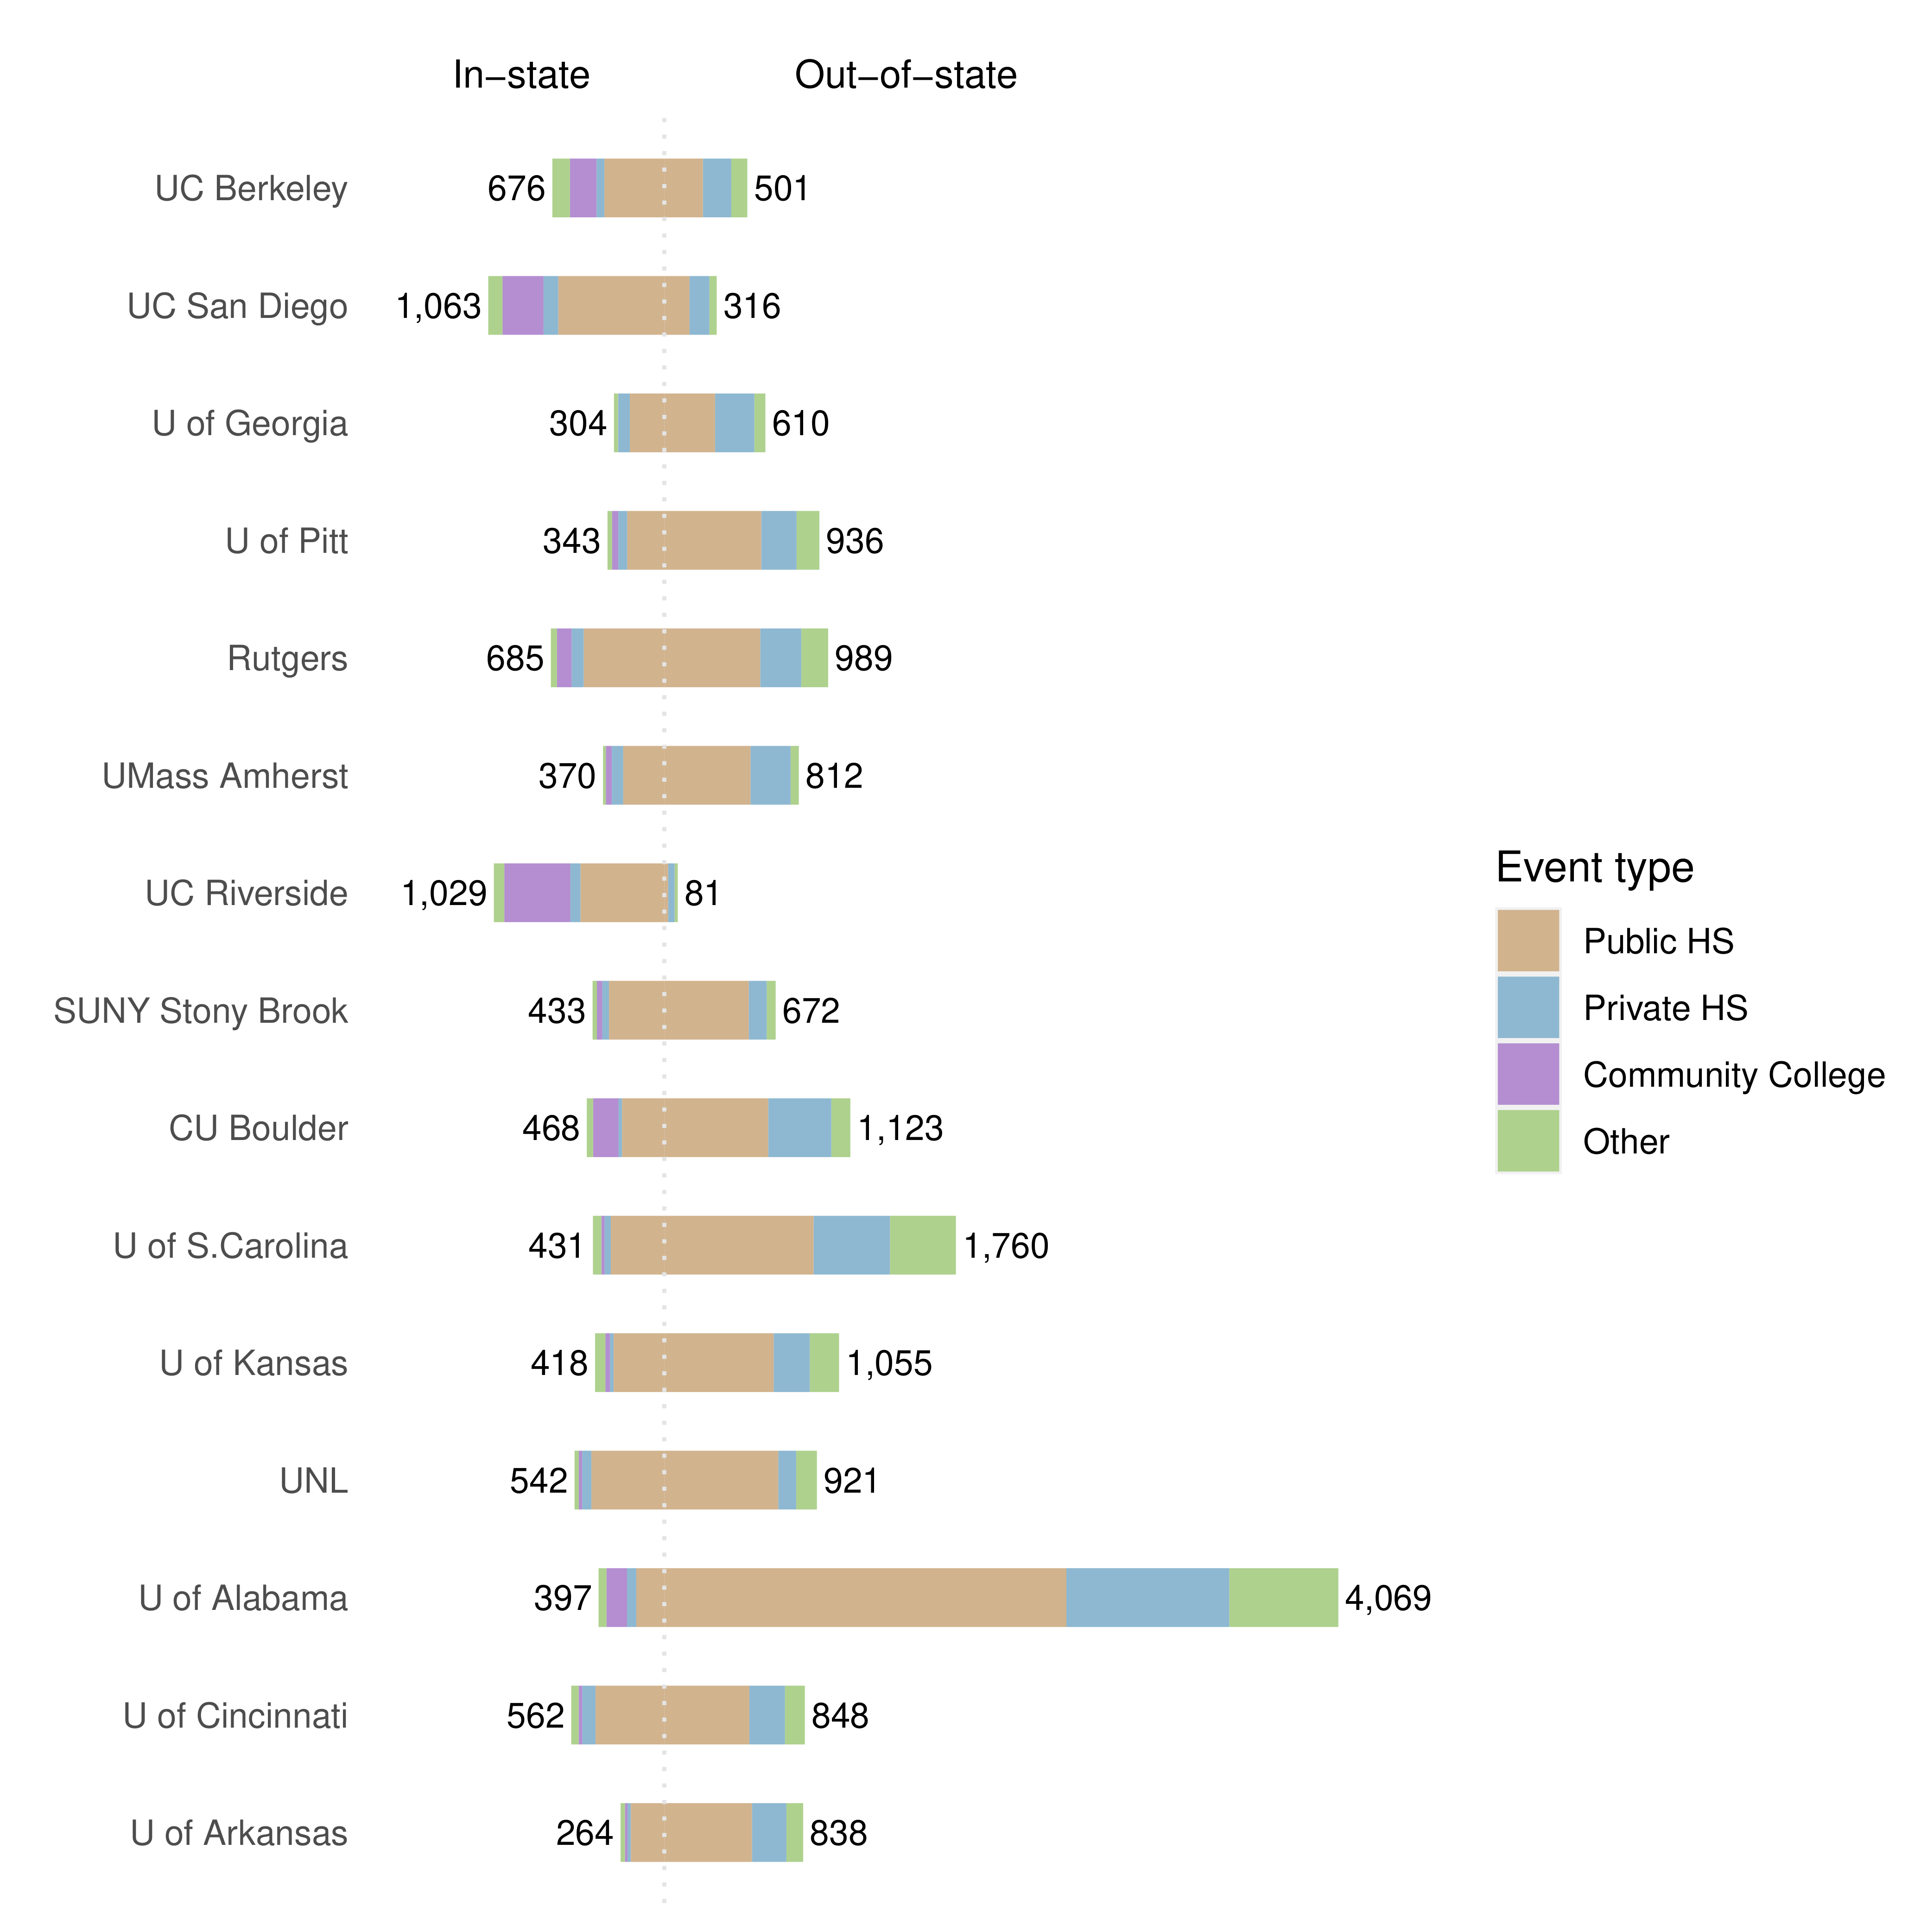
\includegraphics[width=2\linewidth]{../assets/figures/events_count_pubu} 

}

\caption{Number of visits by type and in-state vs. out-of-state, public research universities}\label{fig:events-count-pubu}
\end{figure}

\newpage

\begin{figure}

{\centering 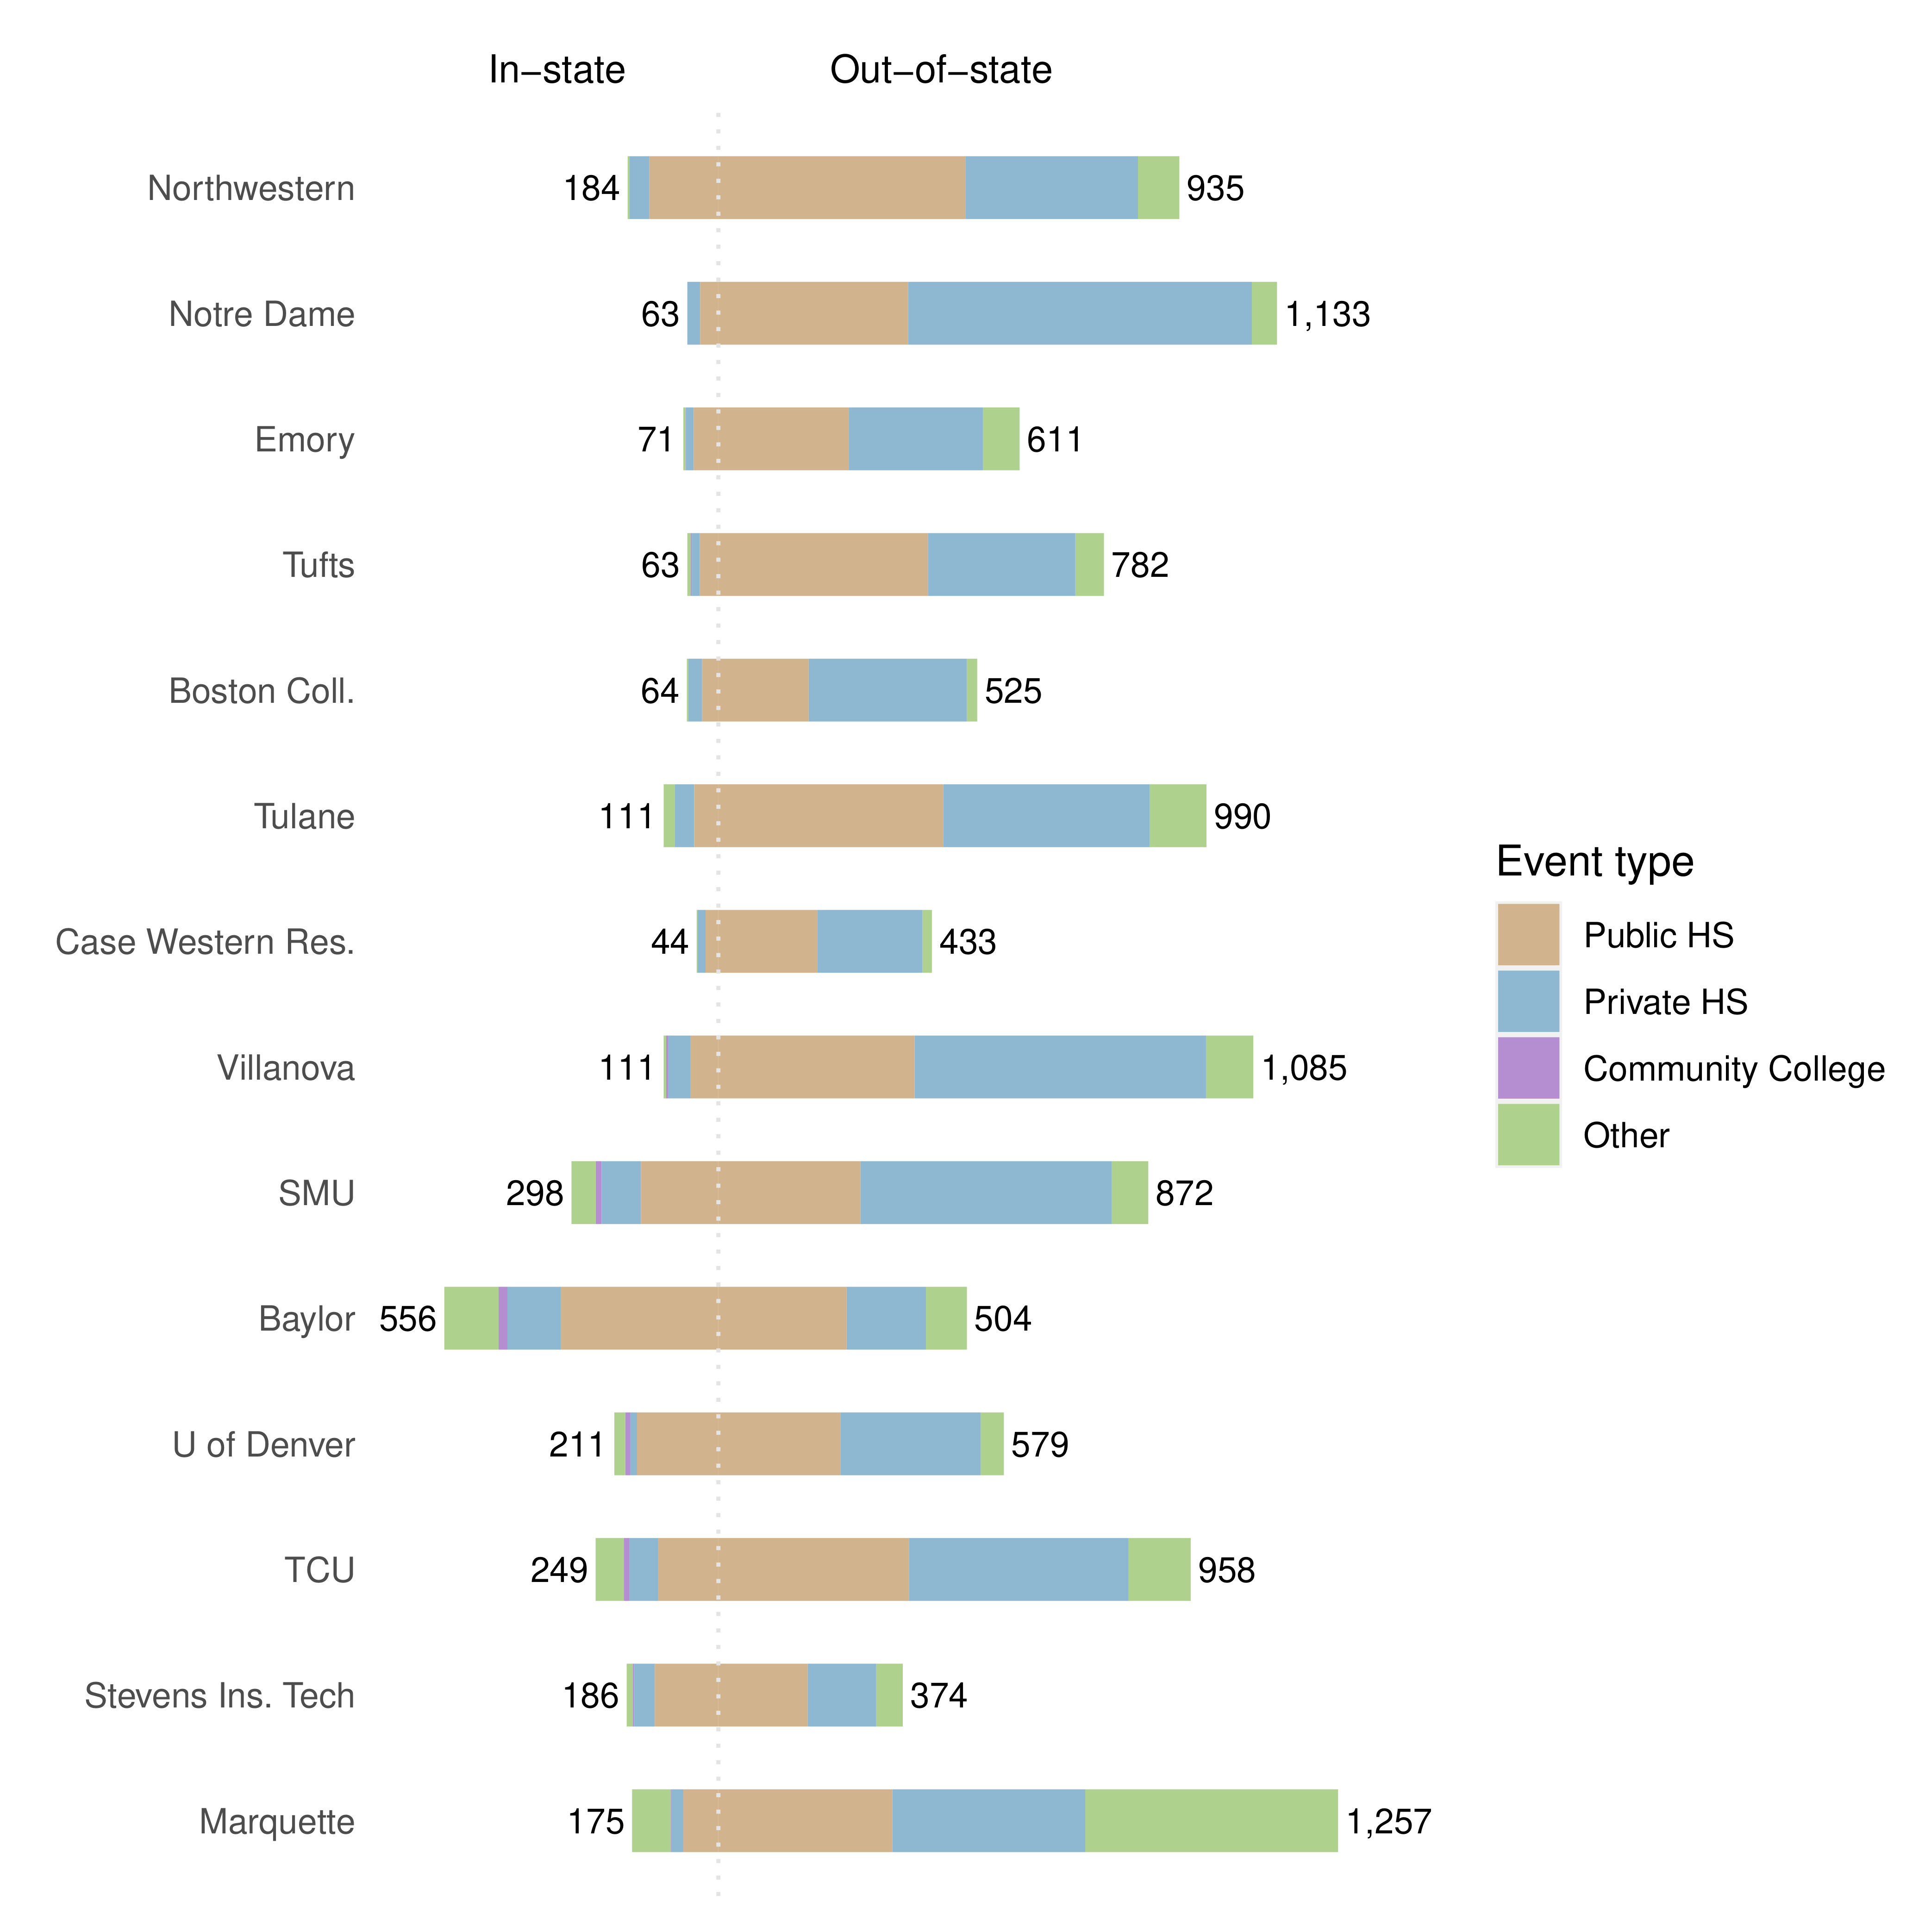
\includegraphics[width=2\linewidth]{../assets/figures/events_count_privu} 

}

\caption{Number of visits by type and in-state vs. out-of-state, selective private universities}\label{fig:events-count-privu}
\end{figure}

\newpage

\begin{figure}

{\centering 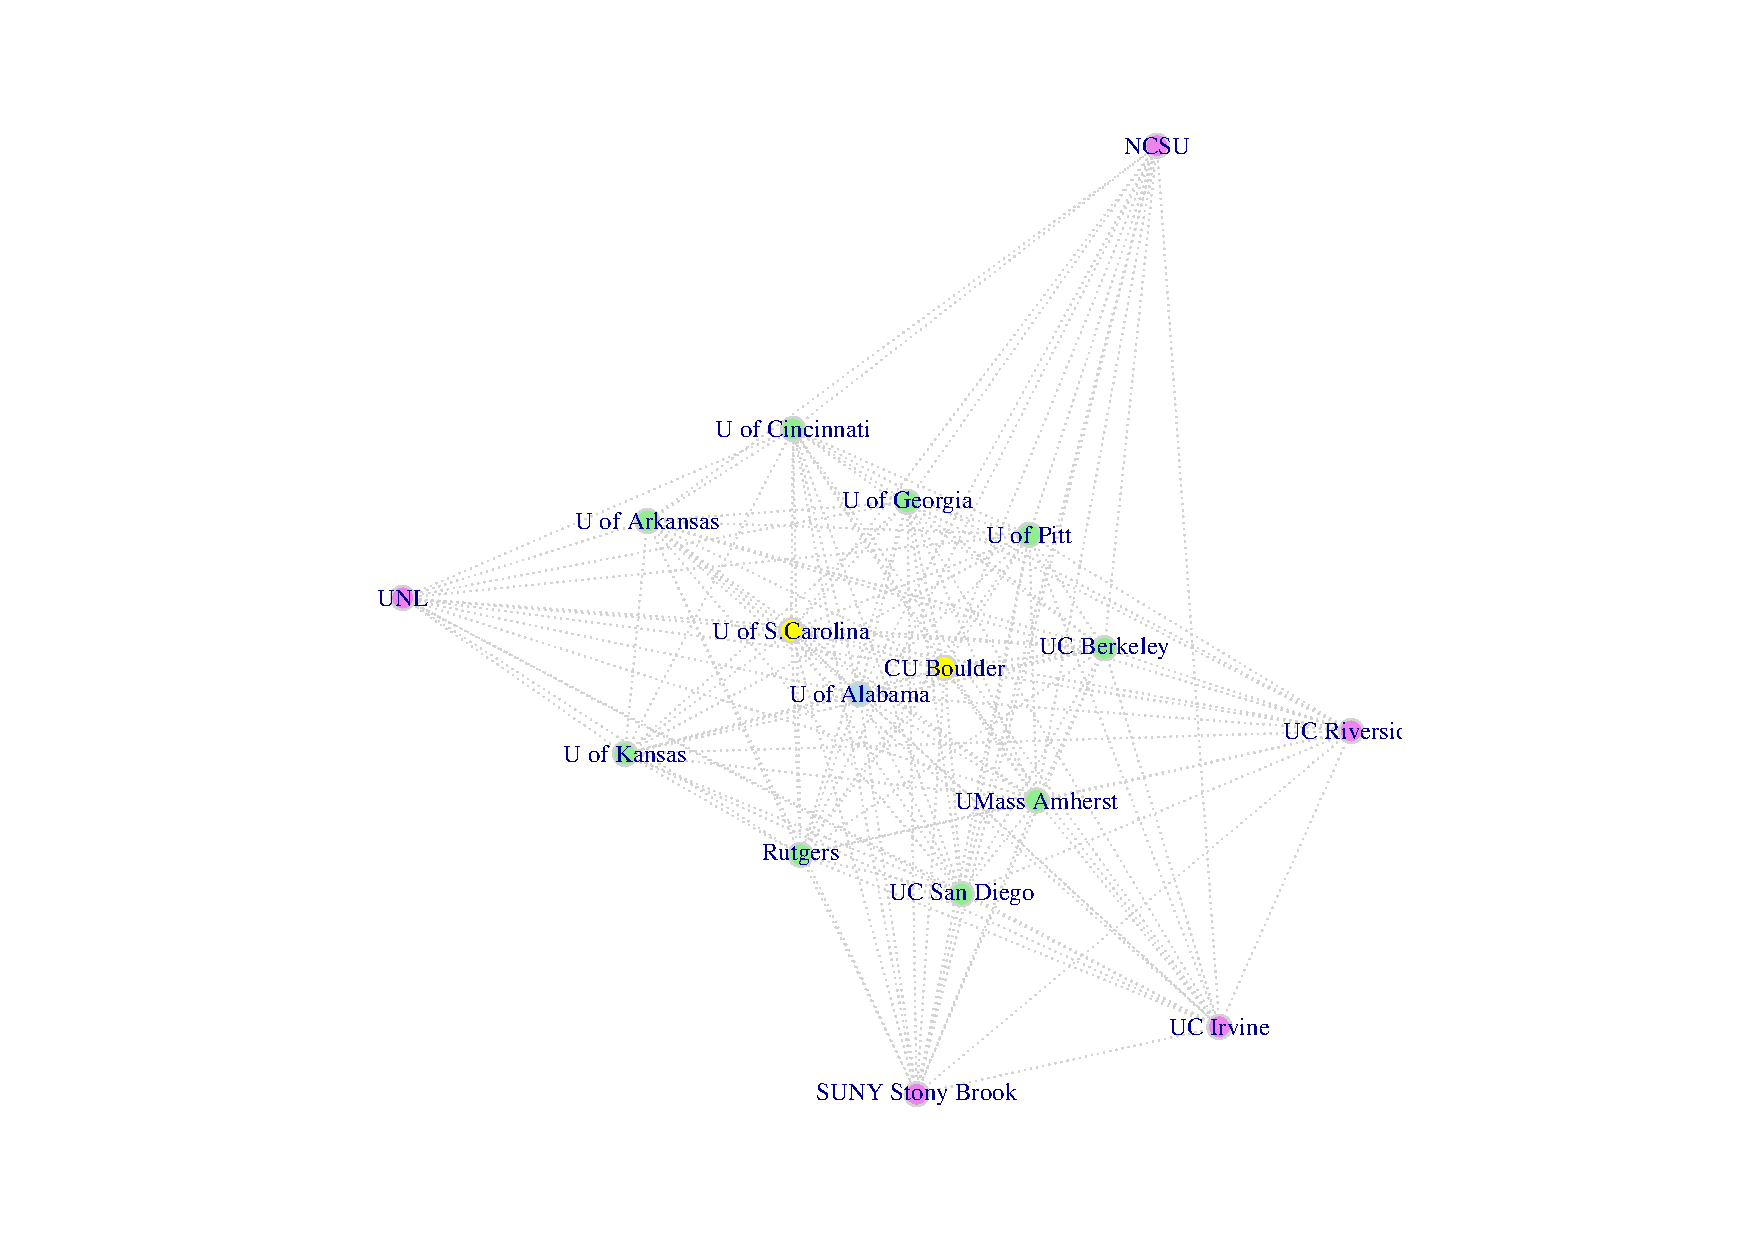
\includegraphics[width=2\linewidth]{../assets/figures/plot_1mode_pubu} 

}

\caption{One-mode network for public research universities, colored by cluster}\label{fig:plot-1mode-pubu}
\end{figure}

\begin{figure}

{\centering 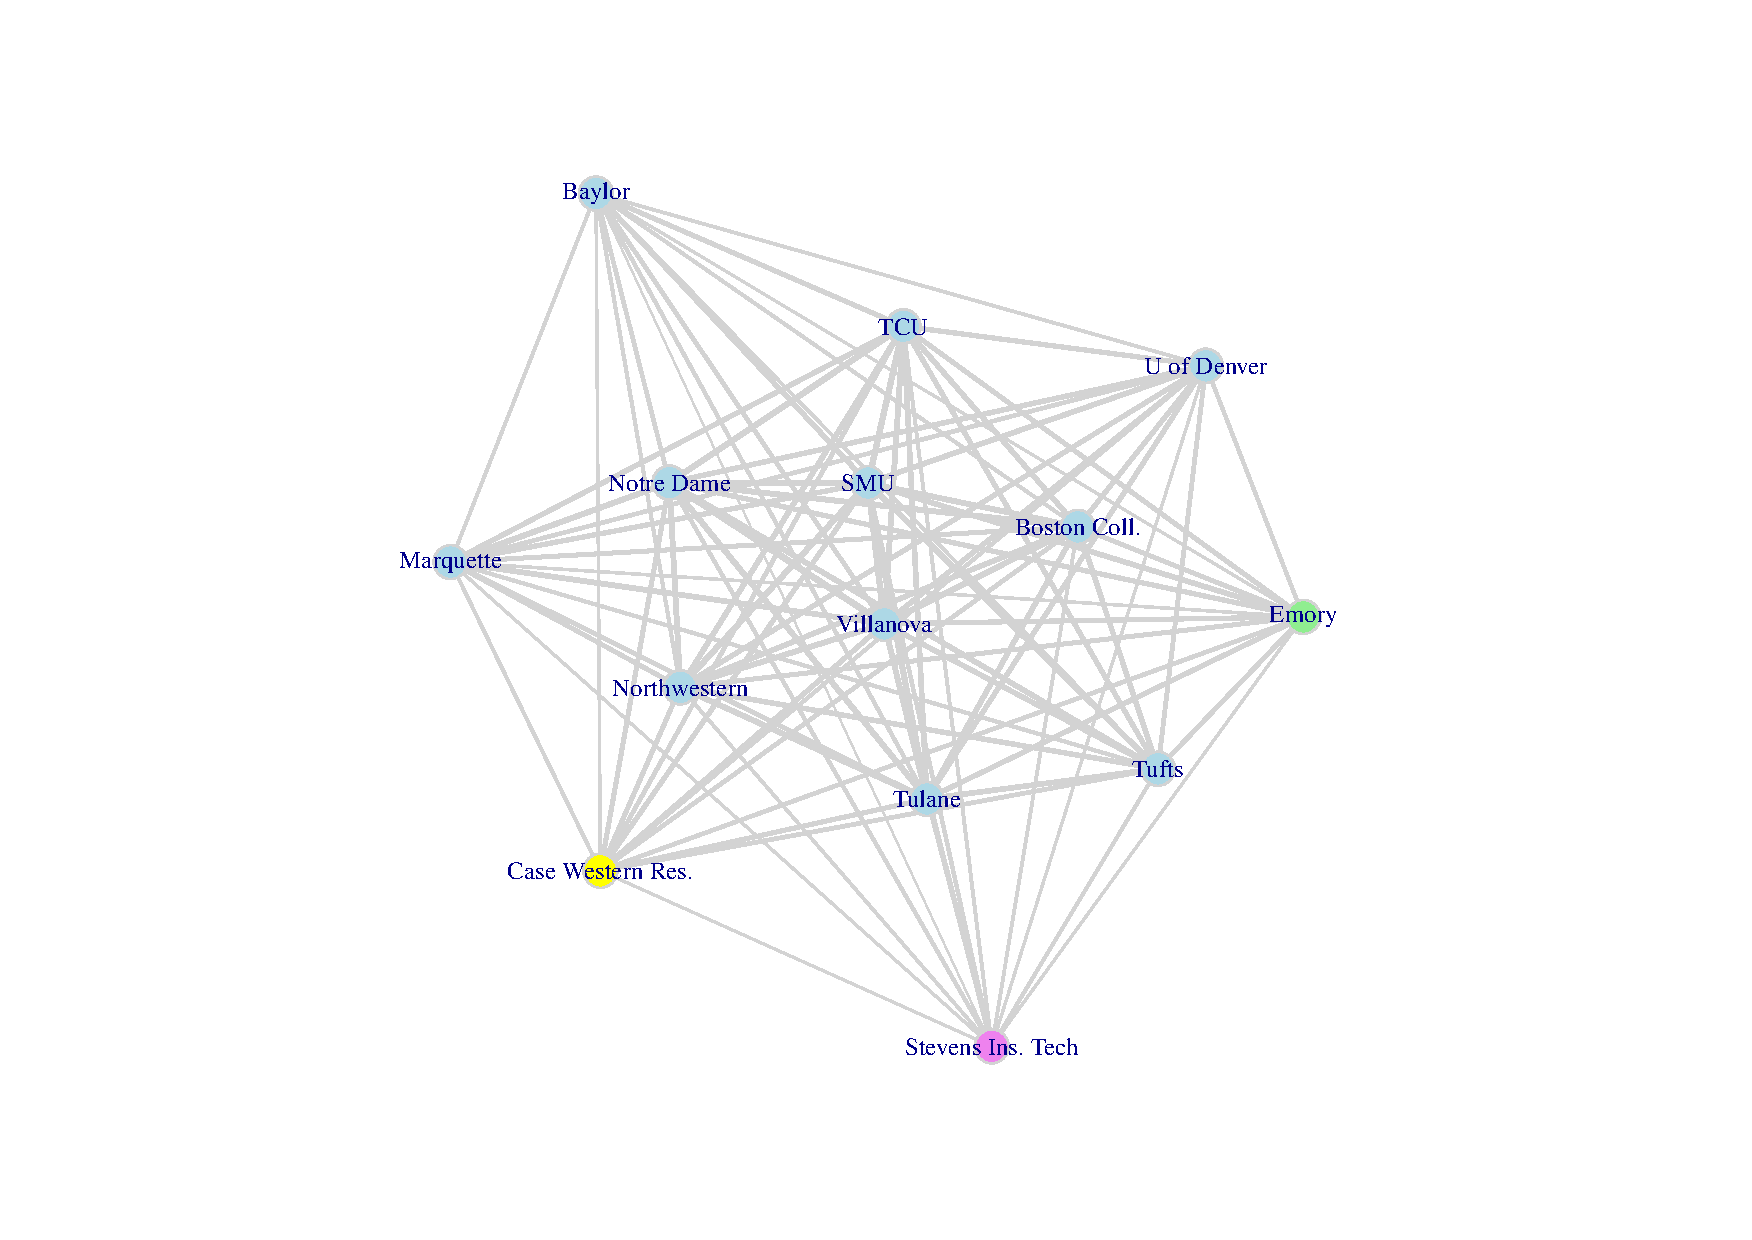
\includegraphics[width=2\linewidth]{../assets/figures/plot_1mode_privu} 

}

\caption{One-mode network for selective private universities, colored by cluster}\label{fig:plot-1mode-privu}
\end{figure}

\newpage


\begin{figure}

{\centering 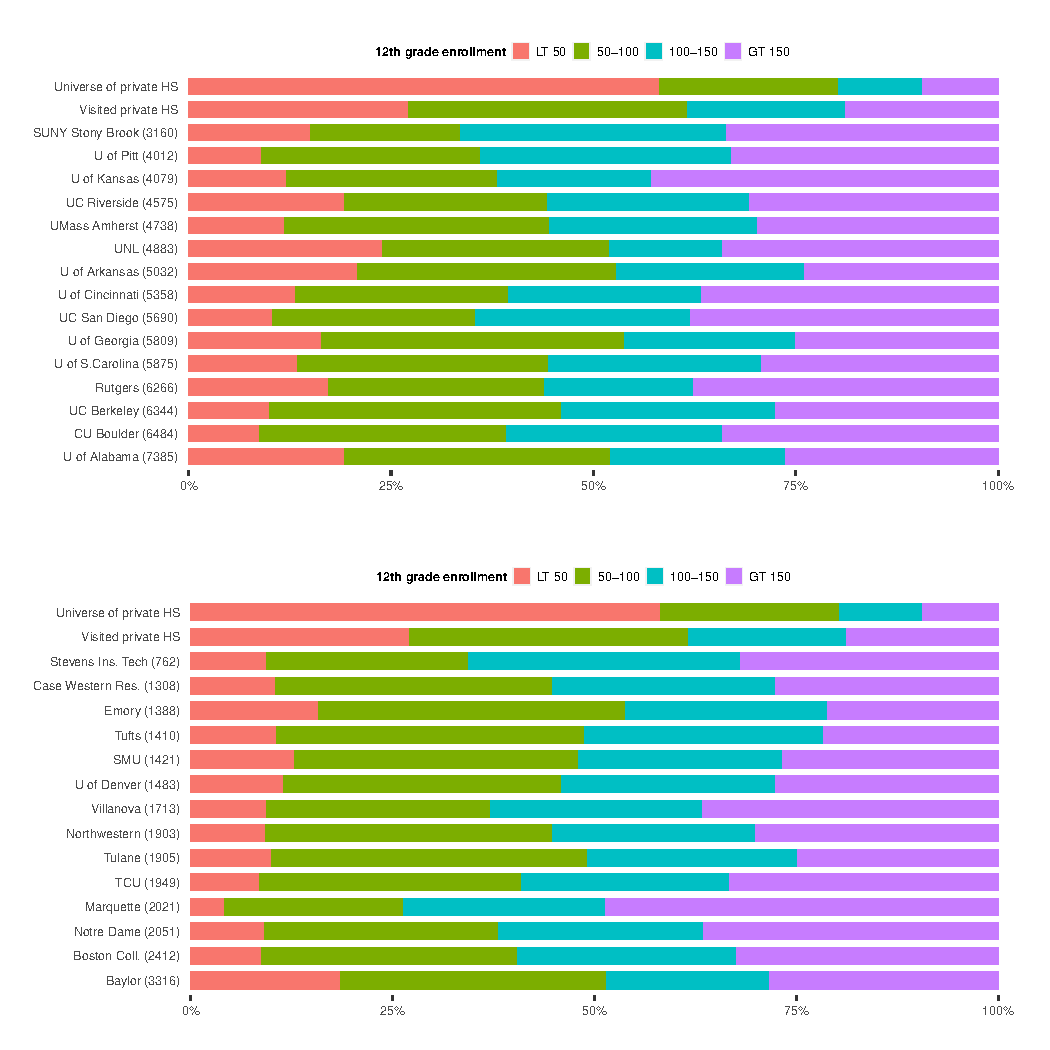
\includegraphics[width=2\linewidth]{../assets/figures/ego_network_enroll_pubu_privu} 

}

\caption{12th grade enrollment of visited private high schools}\label{fig:enroll-pubu-privu}
\end{figure}

\newpage

\begin{figure}

{\centering 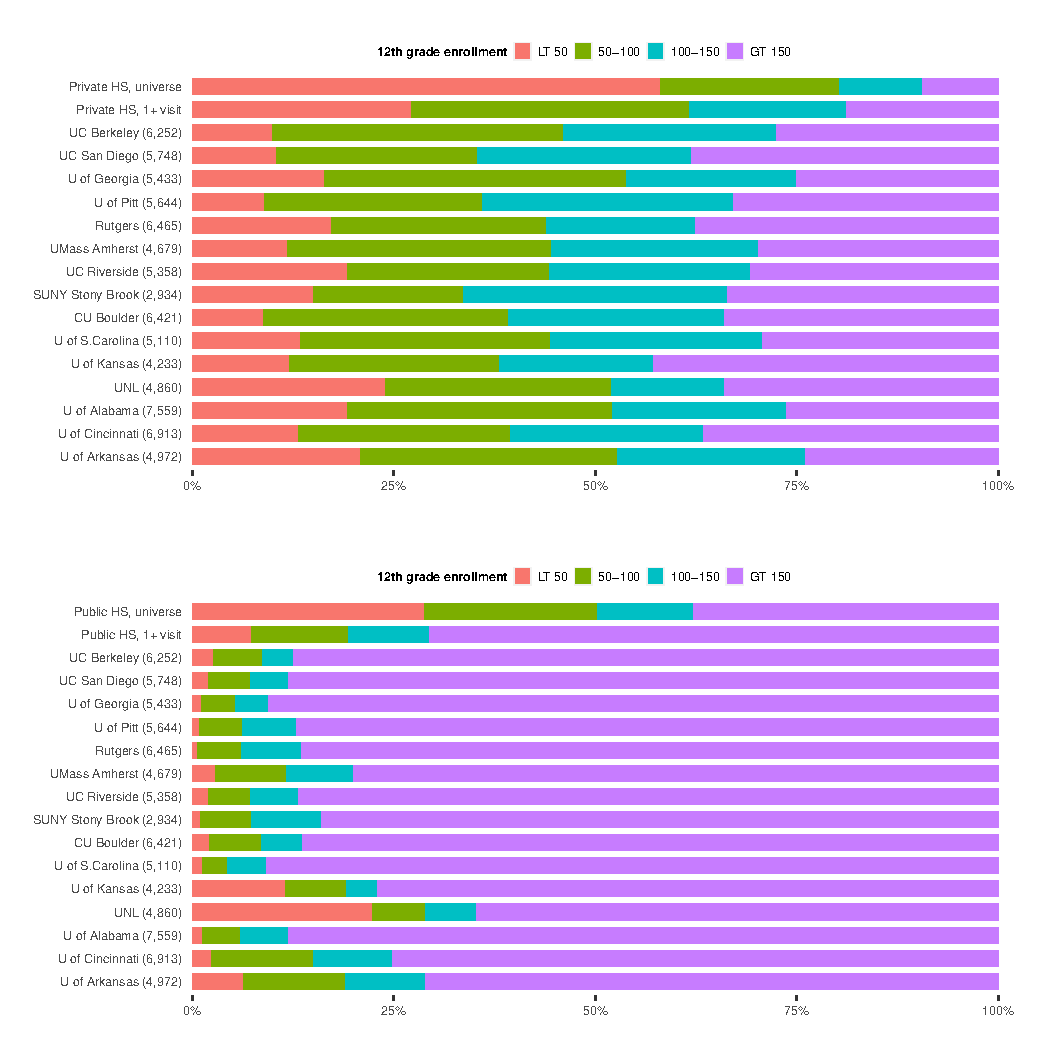
\includegraphics[width=2\linewidth]{../assets/figures/ego_network_enroll_pubu_privhs_pubhs} 

}

\caption{12th grade enrollment of visited private high schools vs. public high schools, public research universities}\label{fig:enroll-pubu-privhs-pubhs}
\end{figure}

\newpage

\begin{figure}

{\centering 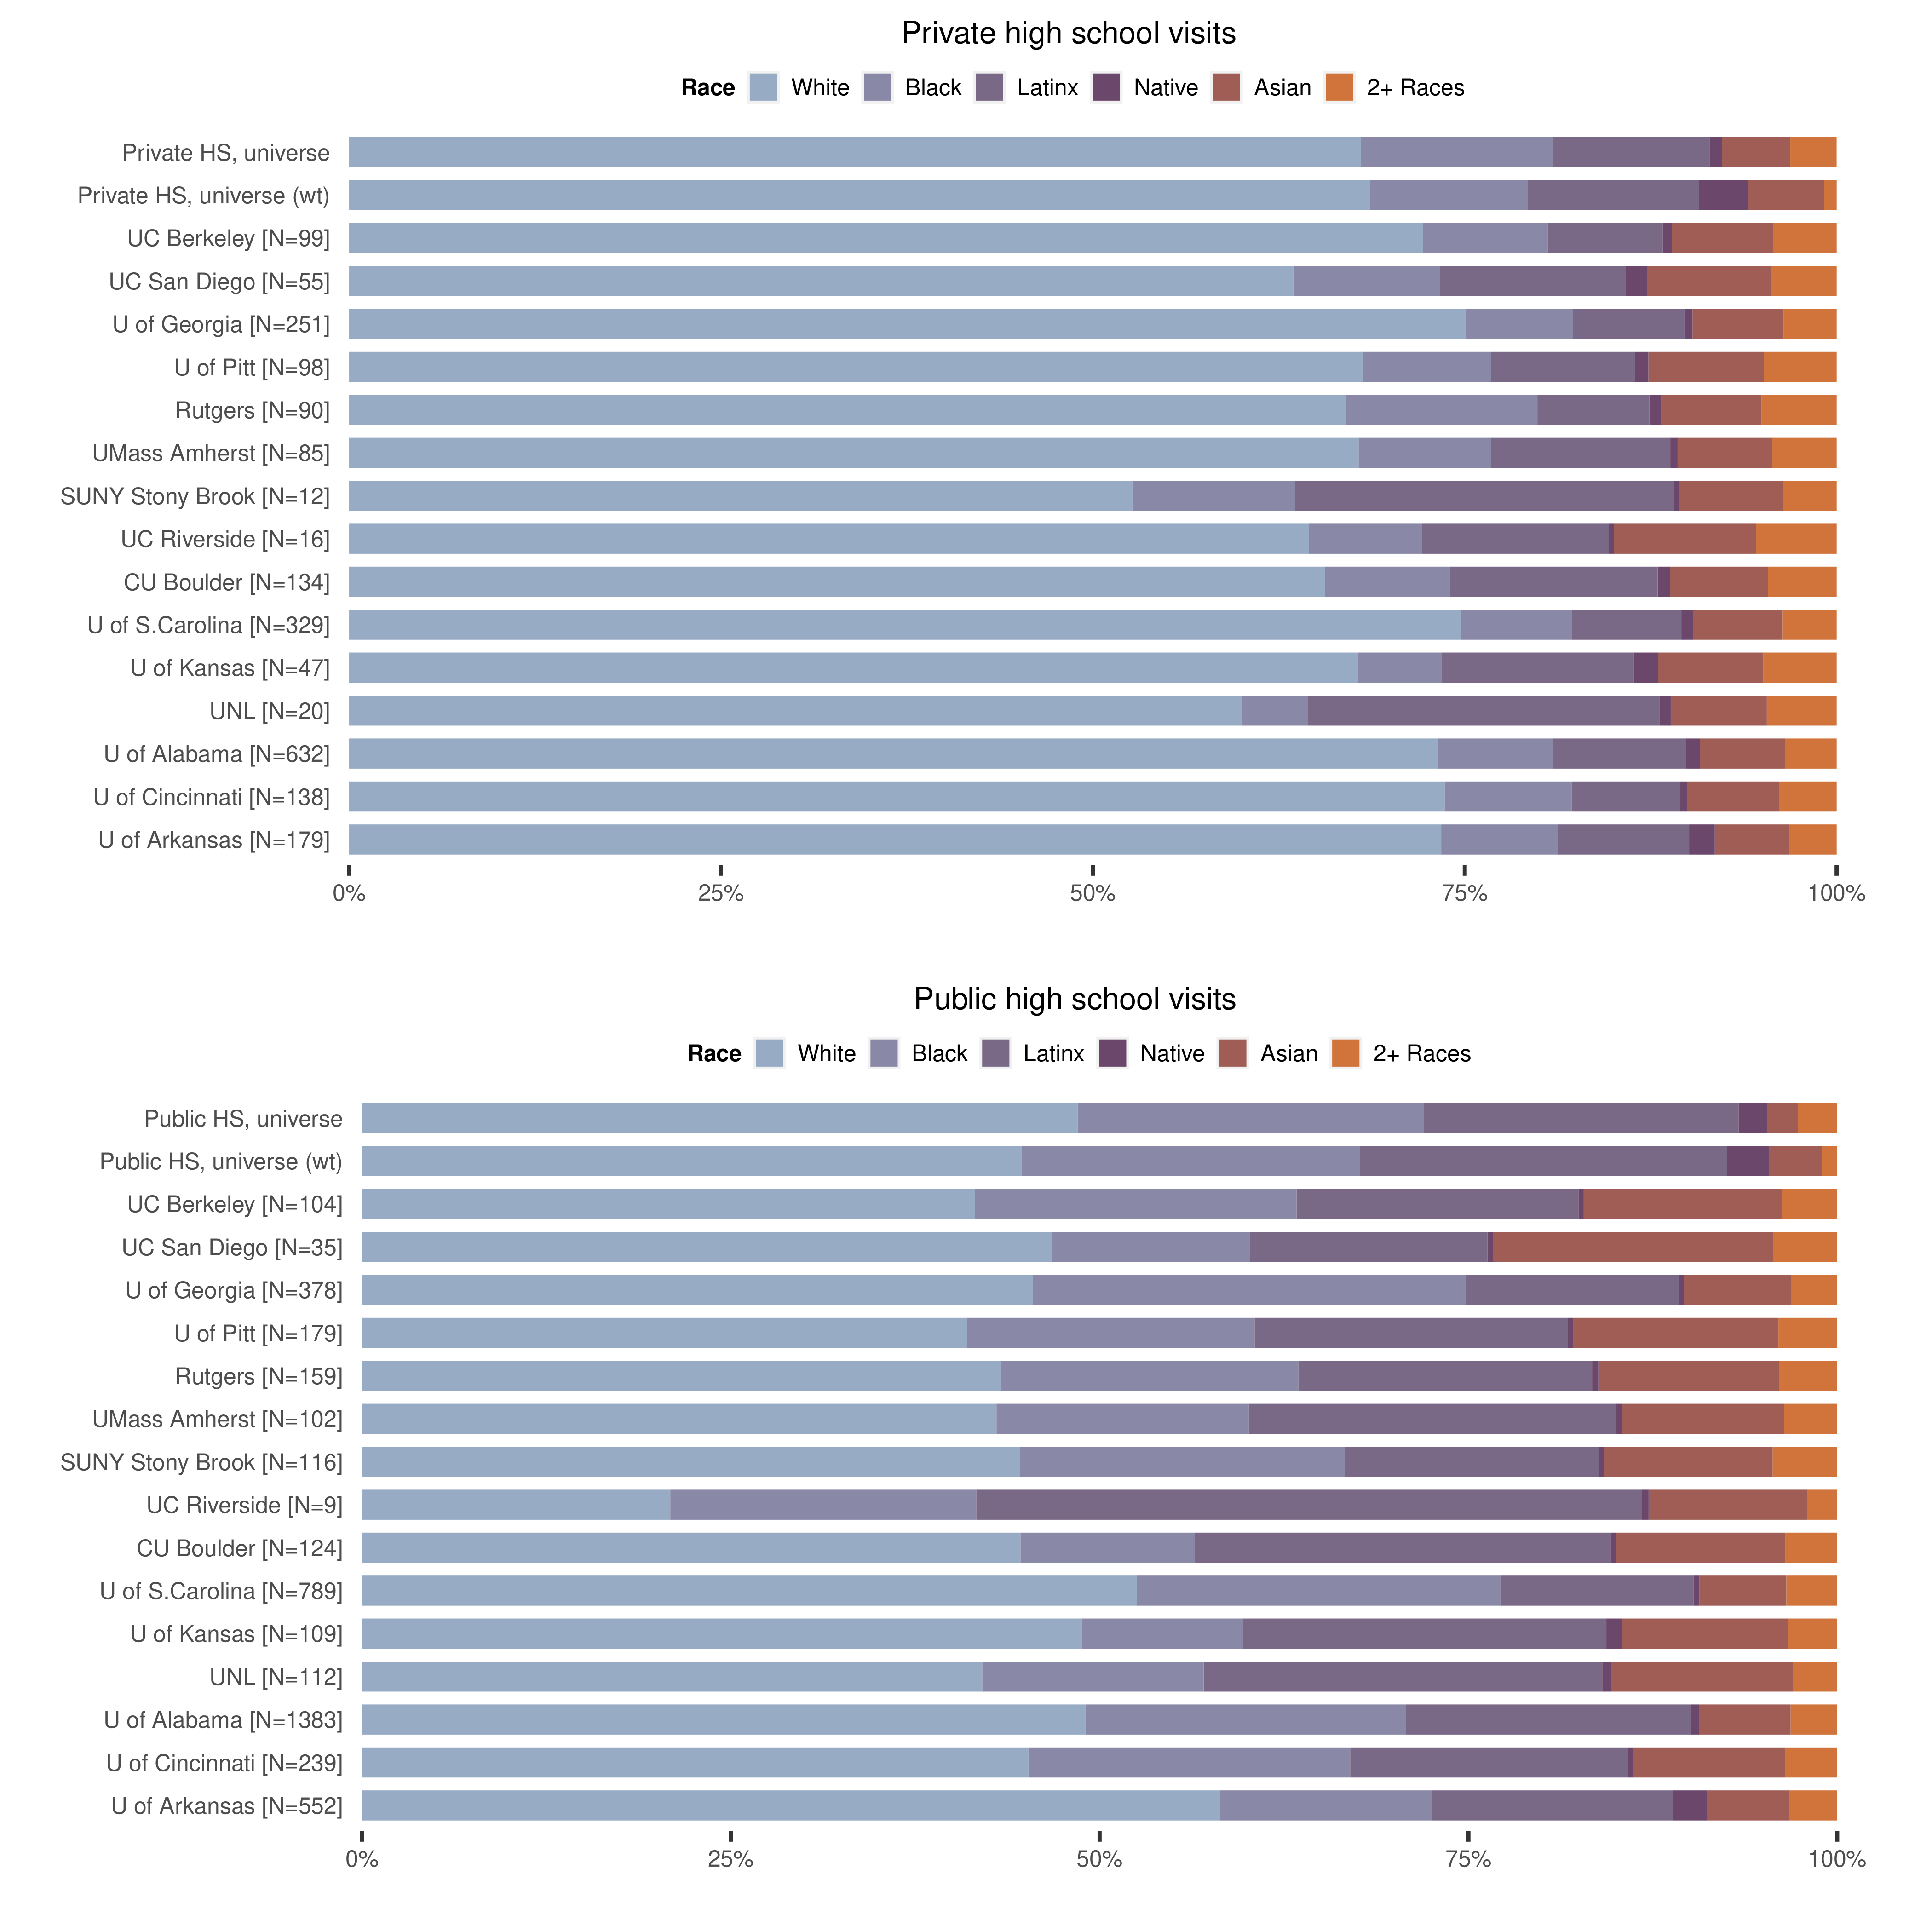
\includegraphics[width=2\linewidth]{../assets/figures/south_race_comp_pubu_privhs_pubhs} 

}

\caption{Racial composition of students at visited public high schools in the South vs. visited private high schools in the South, public research universities}\label{fig:south-race-comp-pubu-privhs-pubhs}
\end{figure}

\newpage

\begin{figure}

{\centering 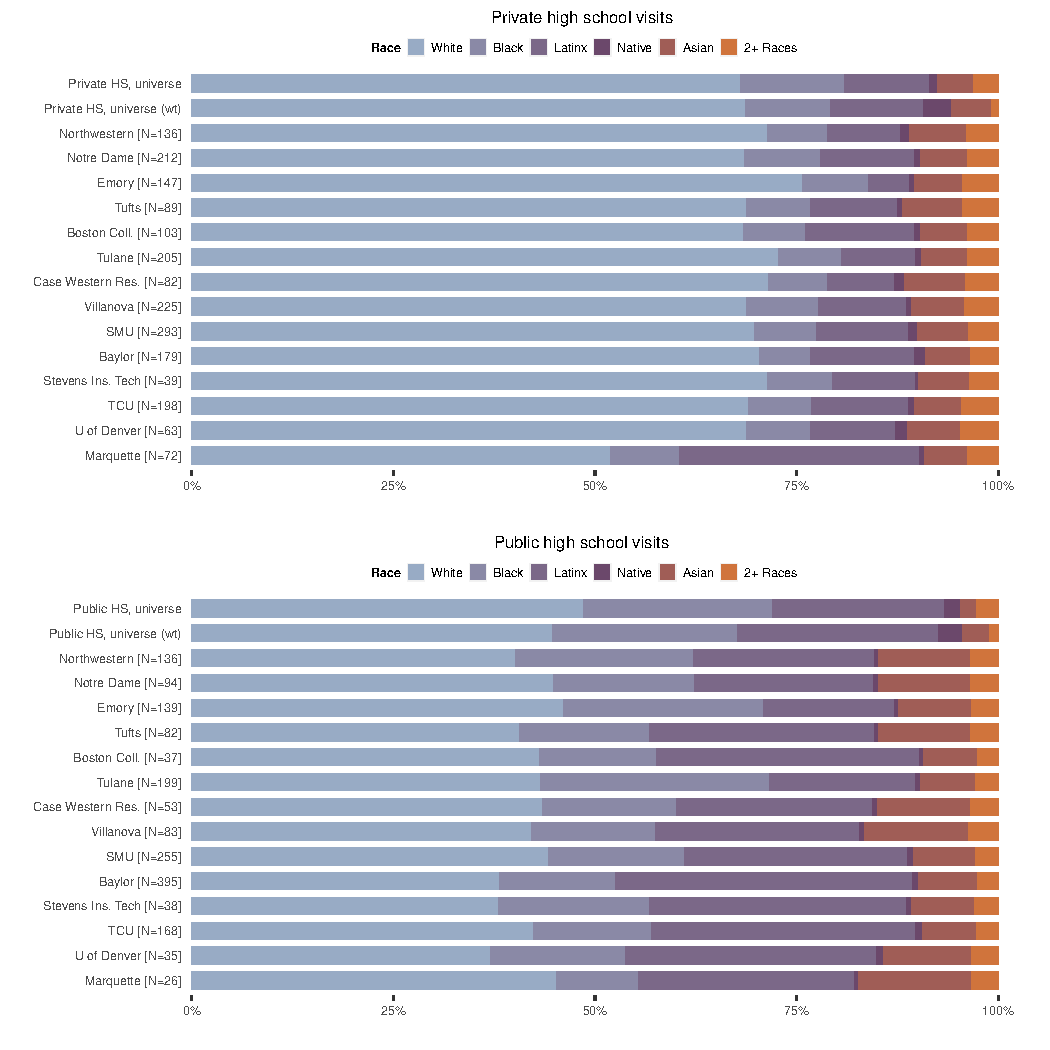
\includegraphics[width=2\linewidth]{../assets/figures/south_race_comp_privu_privhs_pubhs} 

}

\caption{Racial composition of students at visited public high schools in the South vs. visited private high schools in the South, selective private universities}\label{fig:south-race-comp-privu-privhs-pubhs}
\end{figure}

\end{landscape}

\restoregeometry

\end{document}
